\documentclass[12pt]{report}

\setlength {\marginparwidth }{2cm} 

\usepackage{float}
\usepackage[table]{xcolor}
\usepackage{tabulary}
\usepackage{graphicx}
\usepackage{afterpage}

% Definición de colores
\definecolor{mygray}{RGB}{240, 240, 240}

% Creación de página en blanco
\newcommand\blankpage{%
    \null
    \thispagestyle{empty}%
    \addtocounter{page}{-1}%
    \newpage}

% Paquetes LaTeX y estilos globales
\usepackage[utf8]{inputenc}
\usepackage{multicol}
\usepackage{xcolor}
\usepackage{subfigure}
\usepackage[spanish]{babel}
\usepackage[utf8]{inputenc}
\usepackage{graphicx}
\usepackage{titlesec}
\usepackage[bookmarks,breaklinks,colorlinks=true,allcolors=blue]{hyperref}
\usepackage{listings}
\usepackage{inconsolata}
\usepackage{float}

\usepackage[square,numbers]{natbib}
\AtBeginDocument{
  \renewcommand{\bibsection}{\chapter{\bibname}}
} % Bibliografia en capitulo numerado

\usepackage{geometry}
\usepackage{amsmath}
\usepackage{parskip}
\usepackage[official]{eurosym}
\usepackage{todonotes}
\usepackage{csquotes}
% Formato del título de capítulos y secciones
\titleformat{\chapter}[block]{\titlerule[0.8pt]\normalfont\huge\bfseries}{\thechapter.}{.5em}{\Huge}[{\titlerule[0.8pt]}]
\titlespacing*{\chapter}{0pt}{-19pt}{25pt}
\titleformat{\section}[block]{\normalfont\Large\bfseries}{\thesection.}{.5em}{\Large}



% Formato del código fuente con lstlisting
\lstset{
  basicstyle=\ttfamily,
  breaklines=true,
}

% Márgenes
\geometry{
    a4paper,
    margin=2.75cm
}

% Limite de profundidad del índice
\setcounter{tocdepth}{2}

% Indentación de párrafos
\setlength{\parindent}{1cm}

\renewcommand{\lstlistingname}{Extracto de código}
\renewcommand*{\lstlistlistingname}{Índice de extractos de código}

% Comienzo del documento
\begin{document}

    % Portada y secciones no numeradas
    \begin{center}

\vspace*{1cm}


\includegraphics[width=\textwidth]{fig/etsii_us.png}

\vspace*{3cm}
\begin{large}
TRABAJO FIN DE GRADO
\end{large}

\vspace*{0.1in}
\textbf{\huge Desarrollo de una aplicación Android para gestión de estadísticas de partidas y utilidades en juegos de mesa} % Aquí el título de su trabajo

\vspace*{.2in}

{\large Realizado por}\\
\textbf{\Large Jesús Manuel Domínguez Tristancho} % Aquí su nombre

\vspace*{2cm}

\textbf{Para la obtención del título de}\\
{\large Grado en Ingeniería Informática - Tecnologías Informáticas} % Dejar sólo la que corresponda

\vspace*{0.2in}

\textbf{Dirigido por}\\
{\large Rafael Paz Vicente}\\ % Repetir esta línea si hay más de un tutor

\vspace*{0.2in}

\textbf{Realizado en el departamento de}\\
{\large Arquitectura y Tecnología de Computadores}

\vspace*{.6in}
\textbf{\Large Convocatoria de Diciembre, curso 2020/21} % Adaptar al curso en el que presente el trabajo

\end{center}


\thispagestyle{empty} % Impide que se incluya número de página en la portada
\clearpage\setcounter{page}{1} % Comienza a incluir números de página a partir de aquí
\pagenumbering{roman} % En números romanos
    \afterpage{\blankpage}
    \chapter*{Agradecimientos}

Quiero agradecer a todos los profesores y compañeros que me han apoyado y ayudado a cumplir mis objetivos a lo largo de mi vida académica en la universidad.
    \chapter*{Resumen}

Este documento es una memoria de Trabajo de Fin de Grado tratando sobre una aplicación Android que gestiona estadísticas de partidas en juegos de mesas y proporciona varias utilidades para facilitar el transcurso de las partidas.
    \chapter*{Abstract}

This document is an End of Degree Project report dealing with an Android application that manages game statistics in table games and provides various utilities to facilitate the course of the games.
    
    % Índice del documento y de figuras
    \begingroup
        % Los enlaces son normalmente azules, pero en los índices se configuran a negro
        % para que no aparezca todo azul
        \hypersetup{linkcolor=black}
        \afterpage{\blankpage}
        \tableofcontents
        \afterpage{\blankpage}
        \listoffigures
        \afterpage{\blankpage}
        %\lstlistoflistings
    \endgroup
    
    % Cambia el estilo de números de página a normal
    \clearpage\pagenumbering{arabic}
    
    % Capítulos del trabajo
    %\chapter{Ejemplos de uso LaTeX}\label{cap:ejemplos}

\todo[inline]{Este capítulo se incluye únicamente como ayuda y referencia de uso de \LaTeX. No debe aparecer en el documento final.}

\section{Introducción}
En este capítulo se muestran ejemplos de uso de \LaTeX para operaciones comunes. 

\section{Estilos}\label{sec:estilos}
Se pueden aplicar estilos al texto como \textbf{negritas}, \textit{cursiva} y \underline{subrayado}. También se \textcolor{red}{pueden} \textcolor{blue}{aplicar} \textcolor{green}{colores}, y \underline{\textit{combinar}} \textbf{\textcolor{red}{estilos}}. Se recomienda usar sólo negritas para hacer énfasis, y no abusar de este recurso.

\section{Listados}
Con itemize se pueden crear listas no numeradas:

\begin{itemize}
    \item Fresas
    \item Melocotones
    \item Piñas
    \item Nectarinas
\end{itemize}

De manera similar, enumerate permite crear listas numeradas:

\begin{enumerate}
    \item Elaborar la memoria del TFG
    \item Elaborar la presentación
    \item Presentar el TFG
    \item Solicitar el título de Grado
\end{enumerate}

\section{Subsecciones}
Se pueden definir subsecciones con el comando subsection:

\subsection{Primera subsección}\label{sec:subseccion}
Esto es una subsección

\subsection{Segunda subsección}
Esto es otra subsección.

\section{Imágenes y figuras}
Todas las imágenes y figuras del documento se incluirán en la carpeta ``fig''. Se pueden incluir de la siguiente manera:

\begin{figure}[htp]
    \centering
    
\includegraphics[width=0.7\textwidth]{fig/ejemplo.png}
    \caption{Un feroz depredador}
    \label{fig:ejemplo}
\end{figure}

Observe que las figuras se numeran automáticamente según el capítulo y el número de figuras que hayan aparecido anteriormente en dicho capítulo. Existen muchas maneras de definir el tamaño de una figura, pero se aconseja utilizar la mostrada en este ejemplo: se define el ancho de la figura como un porcentaje del ancho total de la página, y la altura se escala automáticamente. De esta manera, el ancho máximo de una figura sería 1.0 * textwidth, lo que aseguraría que se muestra al máximo tamaño posible sin sobrepasar los márgenes del documento.

Tenga en cuenta que LaTeX intenta incluir las figuras en el mismo sitio donde se declaran, pero en ocasiones no es posible por motivos de espacio. En esos casos, LaTeX colocará la figura lo más cerca posible de su declaración, puede que en una página diferente. Esto es un comportamiento normal y no debe ser evitado.

\section{Referencias}
Observe cómo en el código fuente de esta sección se ha usado varias veces el comando ``label''. Este comando permite marcar un elemento, ya sea capítulo, sección, figura, etc. para hacer una referencia numérica al mismo. Para referenciar una ``label'' se usa el comando ``ref'' incluyendo el nombre de la referencia:

Este es el capítulo \ref{cap:ejemplos}.

En la sección \ref{sec:estilos} se muestran ejemplos de estilos.

La subsección \ref{sec:subseccion} explica...

En la Figura \ref{fig:ejemplo} vemos que...

Esto evita que tengamos que escribir directamente los índices de las secciones y figuras que queremos mencionar, ya que LaTeX lo hace por nosotros y además se encarga de mantenerlos actualizados en caso de que cambien (pruebe a mover este capítulo al final del documento y observe cómo se actualizan automáticamente todos los índices referenciados). Además, las referencias mediante ``ref'' actúan como hipervínculos dentro del documento que llevan al elemento referenciado al pulsar en ellas.

Es habitual nombrar las ``label'' con un prefijo que indica el tipo de elemento para encontrarlo luego más fácilmente, pero no es obligatorio.

\section{Extractos de código}

Se pueden incluir extractos de código mediante lstlisting:

\begin{lstlisting}[language=Python, caption={Código Python}, label={cod:python}, captionpos=b]
num = float(input("Enter a number: "))
if num > 0:
   print("Positive number")
elif num == 0:
   print("Zero")
else:
   print("Negative number")
\end{lstlisting}

Se admite gran variedad de lenguajes:

\begin{lstlisting}[language=Java, caption={Código Java}, label={cod:java}, captionpos=b]
public class Test {
    public static void main(String[] args) {
        System.out.println("Hello, world!");
    }
}
\end{lstlisting}

Los extractos de código también se pueden referenciar mediante label/ref: Extractos de código \ref{cod:python} y \ref{cod:java}.

\section{Enlaces}
Puede enlazar una web externa mediante el comando url: \url{https://www.example.com}. También se puede vincular un enlace a un texto mediante el comando href: \href{https://www.example.com}{dominio de ejemplo}.

\section{Citas y bibliografía}
En LaTeX, los elementos de la bibliografía se almacenan en un fichero bibliográfico en un formato llamado BibTeX, en el caso de este proyecto se encuentran en ``bibliografia.bib''. Para citar un elemento se usa el comando ``cite''. Se pueden citar tanto artículos científicos \cite{borrego2019} como enlaces web \cite{webETSII}. Las citas se numeran automáticamente y se incluyen en la sección de bibliografía del documento.

Observe cómo los elementos bibliográficos almacenados en ``bibliografia.bib'' tienen una etiqueta asociada, que es la que se incluye al citarlos mediante cite. Añadir una referencia al fichero bibliográfico no hace que ésta aparezca automáticamente en la sección de bibliografía del trabajo, es necesario citarla en algún lugar del mismo.

\section{Ecuaciones}
LaTeX tiene un potente motor para mostrar ecuaciones matemáticas y un amplio catálogo de símbolos matemáticos. El entorno matemático se puede activar de muchas maneras. Para incluir ecuaciones simples en un texto se pueden rodear de símbolos dólar: $1 + 2 = 3$, $\sqrt{81} = 3^2 = 9$, $\forall x \in y~\exists~z : S_z < 4$.

Las ecuaciones más complejas pueden expresarse aparte y son numeradas: ecuación \ref{eq:ecuacion}.

\begin{equation}\label{eq:ecuacion}
\lim_{x\to 0}{\frac{e^x-1}{2x}}
 \overset{\left[\frac{0}{0}\right]}{\underset{\mathrm{H}}{=}}
 \lim_{x\to 0}{\frac{e^x}{2}}={\frac{1}{2}}
 +7 \int_0^2
  \left(
    -\frac{1}{4}\left(e^{-4t_1}+e^{4t_1-8}\right)
  \right)\,dt_1
\end{equation}

Dispone \href{http://www.yann-ollivier.org/latex/texsymbols.pdf}{aquí} de un amplio listado de símbolos que pueden usarse en modo matemático.

\section{Caracteres y símbolos especiales}
Algunos caracteres y símbolos deben ser escapados para poder representarse en el documento, ya que tienen un significado especial en LaTeX. Algunos de ellos son:

\begin{itemize}
    \item El símbolo dólar \$ se usa para ecuaciones.
    \item El tanto por ciento \% se usa para comentarios en el código fuente.
    \item El símbolo euro \euro{} suele dar problemas si se escribe directamente.
    \item El guión bajo \_ se usa para subíndices en modo matemático.
    \item Las comillas deben expresarse `así' para comillas simples y ``así'' para comillas dobles. Las comillas españolas pueden expresarse \textquote{así}.
    \item La barra invertida o contrabarra \textbackslash{} se usa para comandos LaTeX.
    \item Otros símbolos que deben escaparse son las llaves \{ \}, el ampersand \&, la almohadilla \# y los símbolos mayor que \textgreater{} y menor que \textless{}.
\end{itemize}
    \input{sections/Introducción}
    \input{sections/Elicitación_sistema}
    \input{sections/Diseño}
    \chapter{Implementación}\label{cap:implementacion}

A continuación, se comentarán el entorno de programación como aspectos importantes de la implementación.

\section{Entorno de programación}

El lenguaje de programación escogido ha sido Java. Es un lenguaje de programación y una plataforma informática que fue comercializada por primera vez en 1995 por Sun Microsystems. Hay muchas aplicaciones y sitios web que no funcionarán, probablemente, a menos que tengan Java instalado y cada día se crean más. Java es rápido, seguro y fiable.

La principal razón de la elección de este lenguaje es debido a la preferencia del desarrollador, en este caso el alumno, ya que es uno de los lenguajes que maneja con más eficiencia y ha trabajado en proyectos con una temática similar.

Un entorno de desarrollo integrado, llamado también IDE (siglas en inglés de integrated development environment), es un programa informático compuesto por un conjunto de herramientas de programación. Puede dedicarse en exclusiva a un solo lenguaje de programación o bien puede utilizarse para varios.

Un IDE es un entorno de programación que ha sido empaquetado como un programa de aplicación; es decir, que consiste en un editor de código, un compilador, un depurador y un constructor de interfaz gráfica (GUI). Los IDE pueden ser aplicaciones por sí solas o pueden ser parte de aplicaciones existentes.

Los IDE proveen un marco de trabajo amigable para la mayoría de los lenguajes de programación tales como C++, PHP, Python, Java, C\#, Delphi, Visual Basic, Gambas, etc. 

Como IDE para este proyecto utilizamos Android Studio. Es el entorno de desarrollo integrado oficial para la plataforma Android. Está basado en el software IntelliJ IDEA de JetBrains y ha sido publicado de forma gratuita a través de la Licencia Apache 2.0. Ha sido diseñado específicamente para el desarrollo de Android.

\newpage
    \chapter{Documento de pruebas}\label{cap:documento pruebas}

Las pruebas de software son las investigaciones empíricas y técnicas cuyo objetivo es proporcionar información objetiva e independiente sobre la calidad del producto a la parte interesada.

Las pruebas son básicamente un conjunto de actividades dentro del desarrollo de software. Dependiendo del tipo de pruebas, estas actividades podrán ser implementadas en cualquier momento de dicho proceso de desarrollo.

\section{Formato de las pruebas realizadas}

Estas pruebas constituyen la comprobación de que el código implementado se comporta como debe, sin errores en el código ni problemas en el mismo. También comprenden las pruebas de la integridad de los datos, como puede ser la recuperación de estos y el manejo del acceso con datos incorrectos.

Para el desarrollo de las pruebas seguiré un esquema de formularios donde plantearemos:

\begin{itemize}
    \item La funcionalidad que revisar.
    \item Parte de código o nombre que implementa dicha funcionalidad.
    \item Prueba que realizar.
    \item El resultado que daremos por válido.
    \item El resultado obtenido tras una prueba.
    \item Si la prueba se ha pasado satisfactoriamente.
\end{itemize}

\bigskip

El formato de esta información se presentará en una tabla como la que sigue:

\bigskip

\begin{center}
    \rowcolors{1}{mygray}{white}
    \begin{tabulary}{0.8\textwidth}{L|L}
        \textbf{Apartado} & \textbf{Resultado} \\ \hline
        Funcionalidad que revisar & \hspace{5cm} \\
        Implementado por & \hspace{5cm} \\
        Prueba que realizar & \hspace{5cm} \\
        Resultado válido & \hspace{5cm} \\
        Resultado obtenido & \hspace{5cm} \\
        Prueba satisfactoria & \hspace{5cm} \\
    \end{tabulary} 
\end{center}

\newpage
    \chapter{Plan de pruebas}\label{cap:plan pruebas}

A continuación, presentaré los resultados de las pruebas realizadas en los formatos especificados en el apartado anterior.

\section{Pruebas de código}

\begin{center}
    \rowcolors{1}{mygray}{white}
    \begin{tabulary}{0.8\textwidth}{L|L}
        \textbf{Apartado} & \textbf{Resultado} \\ \hline
        Funcionalidad que revisar & Inicio de conexión con Authentication \\
        Implementado por & FirebaseAuth \\
        Prueba que realizar & Permitir la conexión con Authentication \\
        Resultado válido & Permite la conexión con Authentication \\
        Resultado obtenido & Permite la conexión con Authentication \\
        Prueba satisfactoria & Sí \\
    \end{tabulary} 
\end{center}

\bigskip

\begin{center}
    \rowcolors{1}{mygray}{white}
    \begin{tabulary}{0.8\textwidth}{L|L}
        \textbf{Apartado} & \textbf{Resultado} \\ \hline
        Funcionalidad que revisar & Conexión con la instancia especificada de Authentication \\
        Implementado por & FirebaseAuth\_getInstance \\
        Prueba que realizar & Se conecta con la instancia especificada de Authentication \\
        Resultado válido & Instancia específica de Authentication conectada \\
        Resultado obtenido & Instancia específica de Authentication conectada \\
        Prueba satisfactoria & Sí \\
    \end{tabulary} 
\end{center}

\bigskip

\begin{center}
    \rowcolors{1}{mygray}{white}
    \begin{tabulary}{0.8\textwidth}{L|L}
        \textbf{Apartado} & \textbf{Resultado} \\ \hline
        Funcionalidad que revisar & Inicio de conexión con Realtime Database \\
        Implementado por & FirebaseDatabase \\
        Prueba que realizar & Permitir la conexión con Realtime Database \\
        Resultado válido & Permite la conexión con Realtime Database \\
        Resultado obtenido & Permite la conexión con Realtime Database \\
        Prueba satisfactoria & Sí \\
    \end{tabulary} 
\end{center}

\bigskip

\begin{center}
    \rowcolors{1}{mygray}{white}
    \begin{tabulary}{0.8\textwidth}{L|L}
        \textbf{Apartado} & \textbf{Resultado} \\ \hline
        Funcionalidad que revisar & Conexión con la instancia especificada de Realtime Database \\
        Implementado por & FirebaseDatabase\_getInstance \\
        Prueba que realizar & Se conecta con la instancia especificada de Realtime Database \\
        Resultado válido & Instancia específica de Realtime Database conectada \\
        Resultado obtenido & Instancia específica de Realtime Database conectada \\
        Prueba satisfactoria & Sí \\
    \end{tabulary} 
\end{center}

\bigskip

\begin{center}
    \rowcolors{1}{mygray}{white}
    \begin{tabulary}{0.8\textwidth}{L|L}
        \textbf{Apartado} & \textbf{Resultado} \\ \hline
        Funcionalidad que revisar & Inicio de conexión con las referencias en Realtime Database \\
        Implementado por & DatabaseReference \\
        Prueba que realizar & Permitir la conexión con las referencias en Realtime Database \\
        Resultado válido & Permite la conexión con las referencias en Realtime Database \\
        Resultado obtenido & Permite la conexión con las referencias en Realtime Database \\
        Prueba satisfactoria & Sí \\
    \end{tabulary} 
\end{center}

\bigskip

\begin{center}
    \rowcolors{1}{mygray}{white}
    \begin{tabulary}{0.8\textwidth}{L|L}
        \textbf{Apartado} & \textbf{Resultado} \\ \hline
        Funcionalidad que revisar & Conexión con la Referencia especificada de Realtime Database \\
        Implementado por & DatabaseReference\_getReference \\
        Prueba que realizar & Se conecta con la instancia especificada de Realtime Database \\
        Resultado válido & Referencia específica de Realtime Database conectada \\
        Resultado obtenido & Referencia específica de Realtime Database conectada \\
        Prueba satisfactoria & Sí \\
    \end{tabulary} 
\end{center}

\bigskip

\begin{center}
    \rowcolors{1}{mygray}{white}
    \begin{tabulary}{0.8\textwidth}{L|L}
        \textbf{Apartado} & \textbf{Resultado} \\ \hline
        Funcionalidad que revisar & Mantener conectado al usuario aún cerrando la aplicación \\
        Implementado por & SharedPreferences \\
        Prueba que realizar & Mantener iniciada la sesión \\
        Resultado válido & Inicio de sesión mantenido aunque se cierre la aplicación \\
        Resultado obtenido & Inicio de sesión mantenido aunque se cierre la aplicación \\
        Prueba satisfactoria & Sí \\
    \end{tabulary}
\end{center}

\bigskip

\begin{center}
    \rowcolors{1}{mygray}{white}
    \begin{tabulary}{0.8\textwidth}{L|L}
        \textbf{Apartado} & \textbf{Resultado} \\ \hline
        Funcionalidad que revisar & Edición de las preferencias del SharedPreferences \\
        Implementado por & SharedPreferences\_Editor \\
        Prueba que realizar & Editar las preferencias del SharedPreferences para guardar o no la sesión actual \\
        Resultado válido & Preferencias del SharedPreferences editadas \\
        Resultado obtenido & Preferencias del SharedPreferences editadas \\
        Prueba satisfactoria & Sí \\
    \end{tabulary}
\end{center}

\bigskip

\begin{center}
    \rowcolors{1}{mygray}{white}
    \begin{tabulary}{0.8\textwidth}{L|L}
        \textbf{Apartado} & \textbf{Resultado} \\ \hline
        Funcionalidad que revisar & Modificación de características de las ventanas \\
        Implementado por & requestWindowFeature \\
        Prueba que realizar & Modificar las características de las ventanas \\
        Resultado válido & Características de las ventanas modificada \\
        Resultado obtenido & Características de las ventanas modificada \\
        Prueba satisfactoria & Sí \\
    \end{tabulary}
\end{center}

\bigskip

\begin{center}
    \rowcolors{1}{mygray}{white}
    \begin{tabulary}{0.8\textwidth}{L|L}
        \textbf{Apartado} & \textbf{Resultado} \\ \hline
        Funcionalidad que revisar & Configuración de la barra de la aplicación \\
        Implementado por & getSupportActionBar \\
        Prueba que realizar & Configurar la barra de la aplicación \\
        Resultado válido & Barra de la aplicación configurada \\
        Resultado obtenido & Barra de la aplicación configurada \\
        Prueba satisfactoria & Sí \\
    \end{tabulary}
\end{center}

\bigskip

\begin{center}
    \rowcolors{1}{mygray}{white}
    \begin{tabulary}{0.8\textwidth}{L|L}
        \textbf{Apartado} & \textbf{Resultado} \\ \hline
        Funcionalidad que revisar & Asignación de vistas a las actividades Java \\
        Implementado por & setContentView \\
        Prueba que realizar & Asignar las vistas a las actividades Java \\
        Resultado válido & Vistas a las actividades Java asignadas \\
        Resultado obtenido & Vistas a las actividades Java asignadas \\
        Prueba satisfactoria & Sí \\
    \end{tabulary}
\end{center}

\bigskip

\begin{center}
    \rowcolors{1}{mygray}{white}
    \begin{tabulary}{0.8\textwidth}{L|L}
        \textbf{Apartado} & \textbf{Resultado} \\ \hline
        Funcionalidad que revisar & Creación de una \textit{intención} para iniciar otra actividad \\
        Implementado por & Intent \\
        Prueba que realizar & Crear una \textit{intención} para iniciar otra actividad \\
        Resultado válido & \textit{Intención} para iniciar otra actividad creada \\
        Resultado obtenido & \textit{Intención} para iniciar otra actividad creada \\
        Prueba satisfactoria & Sí \\
    \end{tabulary}
\end{center}

\bigskip

\begin{center}
    \rowcolors{1}{mygray}{white}
    \begin{tabulary}{0.8\textwidth}{L|L}
        \textbf{Apartado} & \textbf{Resultado} \\ \hline
        Funcionalidad que revisar & Adición de claves nuevas en la \textit{intención} que inicia una actividad \\
        Implementado por & Intent\_putExtra \\
        Prueba que realizar & Añadir claves nuevas en la \textit{intención} que inicia una actividad \\
        Resultado válido & Claves nuevas en la \textit{intención} que inicia una actividad añadidas \\
        Resultado obtenido & Claves nuevas en la \textit{intención} que inicia una actividad añadidas \\
        Prueba satisfactoria & Sí \\
    \end{tabulary}
\end{center}

\bigskip

\begin{center}
    \rowcolors{1}{mygray}{white}
    \begin{tabulary}{0.8\textwidth}{L|L}
        \textbf{Apartado} & \textbf{Resultado} \\ \hline
        Funcionalidad que revisar & Devolución de la \textit{intención} que inicia una actividad \\
        Implementado por & getIntent \\
        Prueba que realizar & Devolver la \textit{intención} que inicia una actividad \\
        Resultado válido & \textit{Intención} que inicia una actividad devuelta \\
        Resultado obtenido & \textit{Intención} que inicia una actividad devuelta \\
        Prueba satisfactoria & Sí \\
    \end{tabulary}
\end{center}

\bigskip

\begin{center}
    \rowcolors{1}{mygray}{white}
    \begin{tabulary}{0.8\textwidth}{L|L}
        \textbf{Apartado} & \textbf{Resultado} \\ \hline
        Funcionalidad que revisar & Obtención de claves en la \textit{intención} que inicia la actividad actual \\
        Implementado por & getIntent\_getStringExtra \\
        Prueba que realizar & Obtener claves de la \textit{intención} que inicia la actividad actual \\
        Resultado válido & Claves de la \textit{intención} que inicia la actividad actual obtenidas \\
        Resultado obtenido & Claves de la \textit{intención} que inicia la actividad actual obtenidas \\
        Prueba satisfactoria & Sí \\
    \end{tabulary}
\end{center}

\bigskip

\begin{center}
    \rowcolors{1}{mygray}{white}
    \begin{tabulary}{0.8\textwidth}{L|L}
        \textbf{Apartado} & \textbf{Resultado} \\ \hline
        Funcionalidad que revisar & Búsqueda de una vista por su identificador \\
        Implementado por & findViewById \\
        Prueba que realizar & Buscar una vista por su identificador \\
        Resultado válido & Vista encontrada por su identificador \\
        Resultado obtenido & Vista encontrada por su identificador \\
        Prueba satisfactoria & Sí \\
    \end{tabulary}
\end{center}

\bigskip

\begin{center}
    \rowcolors{1}{mygray}{white}
    \begin{tabulary}{0.8\textwidth}{L|L}
        \textbf{Apartado} & \textbf{Resultado} \\ \hline
        Funcionalidad que revisar & Realización de tareas si se ejecuta la anterior exitosamente \\
        Implementado por & addOnSuccessListener \\
        Prueba que realizar & Realizar tareas si se ejecuta la anterior exitosamente \\
        Resultado válido & Tareas realizadas si la anterior fue exitosa \\
        Resultado obtenido & Tareas realizadas si la anterior fue exitosa \\
        Prueba satisfactoria & Sí \\
    \end{tabulary}
\end{center}

\bigskip

\begin{center}
    \rowcolors{1}{mygray}{white}
    \begin{tabulary}{0.8\textwidth}{L|L}
        \textbf{Apartado} & \textbf{Resultado} \\ \hline
        Funcionalidad que revisar & Realización de tareas si se completó la anterior \\
        Implementado por & addOnCompleteListener \\
        Prueba que realizar & Realizar tareas si se completó la anterior \\
        Resultado válido & Tareas realizadas si la anterior fue completada \\
        Resultado obtenido & Tareas realizadas si la anterior fue completada \\
        Prueba satisfactoria & Sí \\
    \end{tabulary}
\end{center}

\bigskip

\begin{center}
    \rowcolors{1}{mygray}{white}
    \begin{tabulary}{0.8\textwidth}{L|L}
        \textbf{Apartado} & \textbf{Resultado} \\ \hline
        Funcionalidad que revisar & Realización de tareas si ha habido cambios \\
        Implementado por & setOnCheckedChangeListener \\
        Prueba que realizar & Realizar tareas si ha habido cambios \\
        Resultado válido & Tareas realizadas si ha habido cambios \\
        Resultado obtenido & Tareas realizadas si ha habido cambios \\
        Prueba satisfactoria & Sí \\
    \end{tabulary}
\end{center}

\bigskip

\begin{center}
    \rowcolors{1}{mygray}{white}
    \begin{tabulary}{0.8\textwidth}{L|L}
        \textbf{Apartado} & \textbf{Resultado} \\ \hline
        Funcionalidad que revisar & Realización de tareas si el objeto ha sido clicado \\
        Implementado por & setOnClickListener \\
        Prueba que realizar & Realizar tareas si el objeto ha sido clicado \\
        Resultado válido & Tareas realizadas si el objeto ha sido clicado \\
        Resultado obtenido & Tareas realizadas si el objeto ha sido clicado \\
        Prueba satisfactoria & Sí \\
    \end{tabulary}
\end{center}

\bigskip

\begin{center}
    \rowcolors{1}{mygray}{white}
    \begin{tabulary}{0.8\textwidth}{L|L}
        \textbf{Apartado} & \textbf{Resultado} \\ \hline
        Funcionalidad que revisar & Realización de tareas si se escribe alguna consulta \\
        Implementado por & setOnQueryTextListener \\
        Prueba que realizar & Realizar tareas si se escribe alguna consulta \\
        Resultado válido & Tareas realizadas si se escribe alguna consulta \\
        Resultado obtenido & Tareas realizadas si se escribe alguna consulta \\
        Prueba satisfactoria & Sí \\
    \end{tabulary}
\end{center}

\bigskip

\begin{center}
    \rowcolors{1}{mygray}{white}
    \begin{tabulary}{0.8\textwidth}{L|L}
        \textbf{Apartado} & \textbf{Resultado} \\ \hline
        Funcionalidad que revisar & Creación de una barra de navegación \\
        Implementado por & BottomNavigationView \\
        Prueba que realizar & Crear una barra de navegación \\
        Resultado válido & Barra de navegación creada \\
        Resultado obtenido & Barra de navegación creada \\
        Prueba satisfactoria & Sí \\
    \end{tabulary}
\end{center}

\bigskip

\begin{center}
    \rowcolors{1}{mygray}{white}
    \begin{tabulary}{0.8\textwidth}{L|L}
        \textbf{Apartado} & \textbf{Resultado} \\ \hline
        Funcionalidad que revisar & Cambio de vista clicando sobre la barra de navegación \\
        Implementado por & BottomNavigationView\_OnNavigationItemSelectedListener \\
        Prueba que realizar & Cambiar de vista clicando sobre la barra de navegación \\
        Resultado válido & Vista cambiada clicando sobre la barra de navegación \\
        Resultado obtenido & Vista cambiada clicando sobre la barra de navegación \\
        Prueba satisfactoria & Sí \\
    \end{tabulary}
\end{center}

\bigskip

\begin{center}
    \rowcolors{1}{mygray}{white}
    \begin{tabulary}{0.8\textwidth}{L|L}
        \textbf{Apartado} & \textbf{Resultado} \\ \hline
        Funcionalidad que revisar & Mostración de mensajes hacia el usuario \\
        Implementado por & Toast \\
        Prueba que realizar & Mostrar mensajes hacia el usuario \\
        Resultado válido & Mensajes hacia el usuario mostrados \\
        Resultado obtenido & Mensajes hacia el usuario mostrados \\
        Prueba satisfactoria & Sí \\
    \end{tabulary}
\end{center}

\newpage
    \input{sections/Planificación}
    \chapter{Conclusiones}\label{cap:conclusiones}

A pesar de la situación actual y los problemas que derivan de ella, las conclusiones que saco del proyecto son positivas. Elegí este proyecto porque quería realizar un desarrollo desde cero creando un producto final que fuese usado por un grupo de personas y contribuyese a facilitar el trabajo.

Hablando del desarrollo de la aplicación en general, puedo decir que aun teniendo conocimientos previos sobre aplicaciones Android, se notó la falta de experiencia en el desarrollo de aplicaciones desde cero. Este problema se pudo solucionar mediante la experiencia y el manejo que iba obteniendo mientras progresaba en el proyecto.

Si hablamos sobre los objetivos comentados al principio de este documento, podemos decir que se han cumplido todos los objetivos deseados: 

\begin{enumerate}
    \item Las estadísticas de las partidas en los juegos de mesa son guardadas en una base de datos Firebase completamente en línea.
    \item Estas estadísticas son diferenciadas entre cada participante de dicha partida, es decir, a cada participante se le asigna únicamente sus puntuaciones y las de nadie más.
    \item Al ser una base de datos completamente en línea, el usuario puede obtener todos sus progresos independientemente del dispositivo que esté utilizando.
    \item El usuario tiene a su alcance herramientas para lanzar una gran cantidad y de diferentes tipos de dados, puede contar puntuaciones en directo, hacer uso de los diferentes contadores para juegos de cartas que requieren contadores para múltiples características y poder calcular el tiempo sin la necesidad de estar cambiando de aplicación continuamente.
    \item La aplicación usa la red del dispositivo para obtener y guardar los datos de la base de datos, mientras que puede usar las diferentes herramientas sin tener acceso a internet.
\end{enumerate}


    \chapter{Trabajo futuro}\label{cap:trabajo futuro}

Los objetivos principales de este trabajo han sido completado como se menciona anteriormente. Aún así, se han pensado algunas mejoras que se le podría implementar a esta aplicación.

\begin{enumerate}
    \item \textbf{Usar aplicación completa de forma local:} la aplicación tiene su base de datos de forma \textit{online} y a tiempo real, esto implica a que se necesite internet cada vez que se quiera usar, pero se podría hacer uso de SQL Lite u otra base de datos local para que mantuviera lo existente para usos \textit{offline} y se actualizara una vez se tuviera acceso a internet.
    
    \item \textbf{Gráficas para representar puntuaciones:} las puntuaciones se nos muestran con forma de "bocadillo" mostrándonos la puntuación, la posición y una corona si hemos quedado primero, pero otra forma de mostrar estas puntuaciones, partidas ganadas, perdidas o jugadas en un año, mes o día específico, etc. Sería mediante gráficas. Esto haría que fuera de una forma más visual y sencilla la representación de estos números.
    
    \item \textbf{Más conectividad entre usuarios:} actualmente, la conectividad entre usuarios es mínima. La única conexión que tienen es cuando crean una nueva partida y escriben como participante a otro usuario. Por ello, se podría crear una sección de comentarios de partidas para los usuarios que sean participantes de dichas partidas, valoraciones a las partidas, agregar amigos, ver resultados y partidas de amigos, etc.
    
    \item \textbf{Animaciones y sonidos para la alarma:} en la sección de utilidades tenemos una herramienta que se llama\textit{Cronómetro}, pero no destaca mucho. Para ello, se podría rediseñar con animaciones cuando clicas en alguno de los botones de \textit{play, pausa} o \textit{replay}, o que el circulo que hay alrededor gire, por ejemplo. Además, también se le podrían incluir pitos cada 10 segundos o 1 minuto.
    
    \item \textbf{Lista de juegos expandible por usuarios:} la lista de juegos se obtiene mediante una API, pero siempre puede quedar algún juego fuera de esta API. Por ello, estaría bien implementar una funcionalidad para que los usuarios hagan peticiones para implementar juegos a la lista.
    
    \item \textbf{Subir aplicación a PlayStore:} por último, lo que se podría hacer para mejorar un poco más la aplicación sería dar a los usuarios un método sencillo para poder instalar la aplicación en sus dispositivos sin tener que descargar un archivo .APK. Para ello, la solución más fácil sería subir la aplicación a la PlayStore de Android.
\end{enumerate}
    \input{sections/Bibliografía}
    \chapter{Anexos}\label{cap:manual}

En esta sección se comentará como desplegar la aplicación desarrollada y, posteriormente, un manual de cómo usar sus funcionalidades.

\section{Manual de instalación}

El despliegue para este caso tendrá un nivel de dificultad muy bajo porque se trata de una instalación en dispositivos móviles con Android como sistema operativo. Para ello, el desarrollador le proporcionará al cliente un instalador (un archivo con formato APK) el cual únicamente tendrá que ser ejecutado y confirmar que desea instalar dicha aplicación en su dispositivo.

También se planteó la opción de subir la aplicación a la PlayStore de Android, pero se requieren 25€ para obtener una cuenta de desarrollador Android con los permisos necesarios para subir aplicaciones a la PlayStore.

Importante destacar que es necesario que el dispositivo móvil tenga instalados los servicios de Google, debido a que la base de datos utilizada proviene de Google y no se puede usar si no se tienen dichos servicios instalados. Esto quiere decir que en dispositivos como los últimos lanzados por la marca Huawei que no traen instalados de fábrica estos servicios, no podrán usar dicha aplicación.

Lo que ocurre exactamente es que al usuario cuando intenta registrarse o iniciar sesión con una cuenta creada en otro dispositivo, la aplicación le va a mostrar por pantalla un mensaje comunicándole que ha habido un fallo en el intento de iniciar sesión.

\section{Manual de uso}

\subsection{Introducción}\label{sec:Uso}

Para explicar el uso de la aplicación iremos siguiendo los siguiente pasos marcados en el orden en el que se va describiendo, aunque el usuario siempre puede ejecutar la aplicación como él crea conveniente para su comodidad y disfrute.

\subsection{Uso paso a paso}

Una vez instalada la aplicación, lo primero que verá el usuario al abrir la aplicación será esta ventana donde podremos escribir nuestro correo y la contraseña para iniciar sesión. 

\begin{figure}[H]
    \centering
    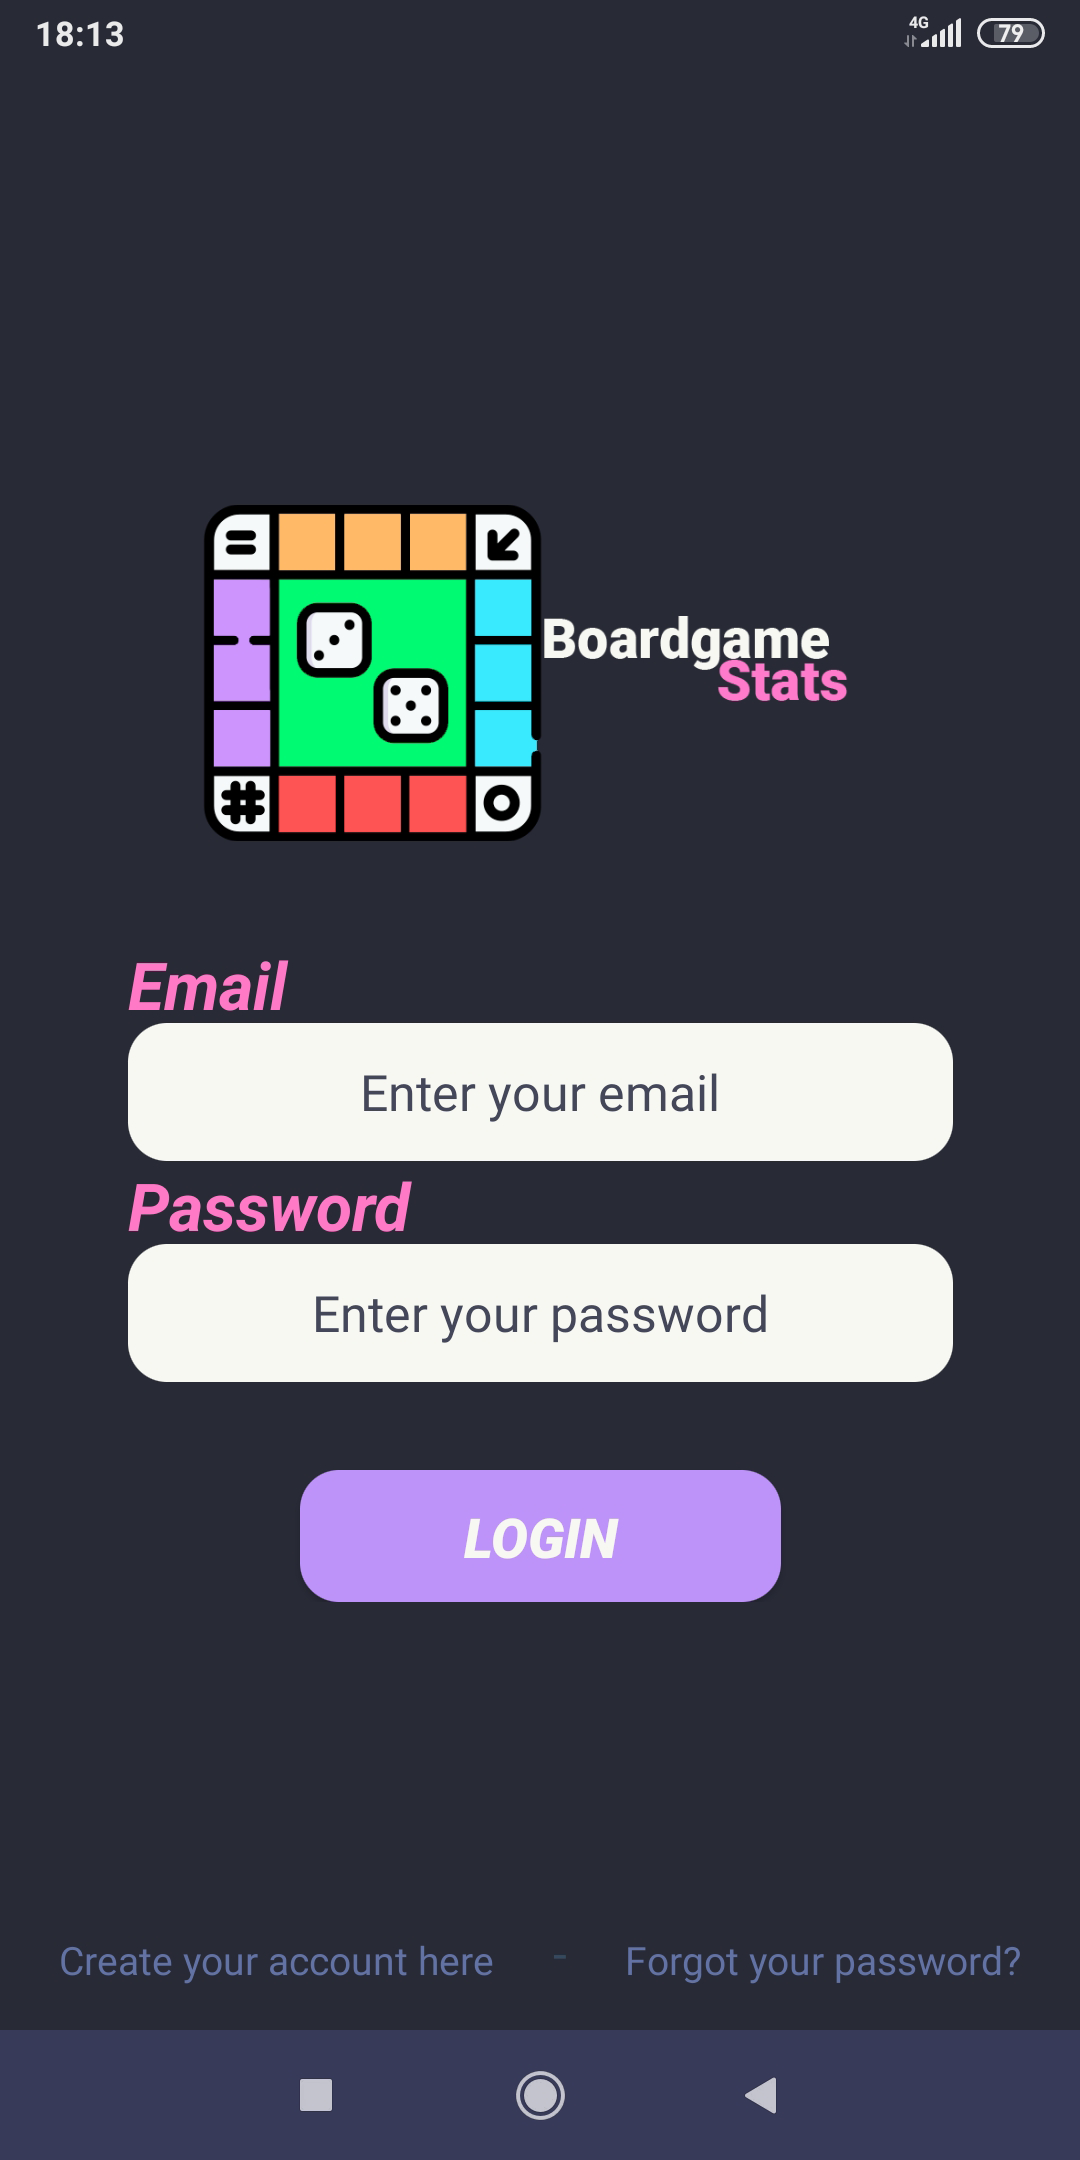
\includegraphics[width=0.3\linewidth]{fig/Uso/1.png}
    \caption{Inicio de sesión}
    \label{fig:uso1}
\end{figure}

Este no es el caso, por lo que primero deberemos registrarnos. Para ello vamos a pulsar el botón que se nos muestra reflejado en la siguiente figura.

\begin{figure}[H]
    \centering
    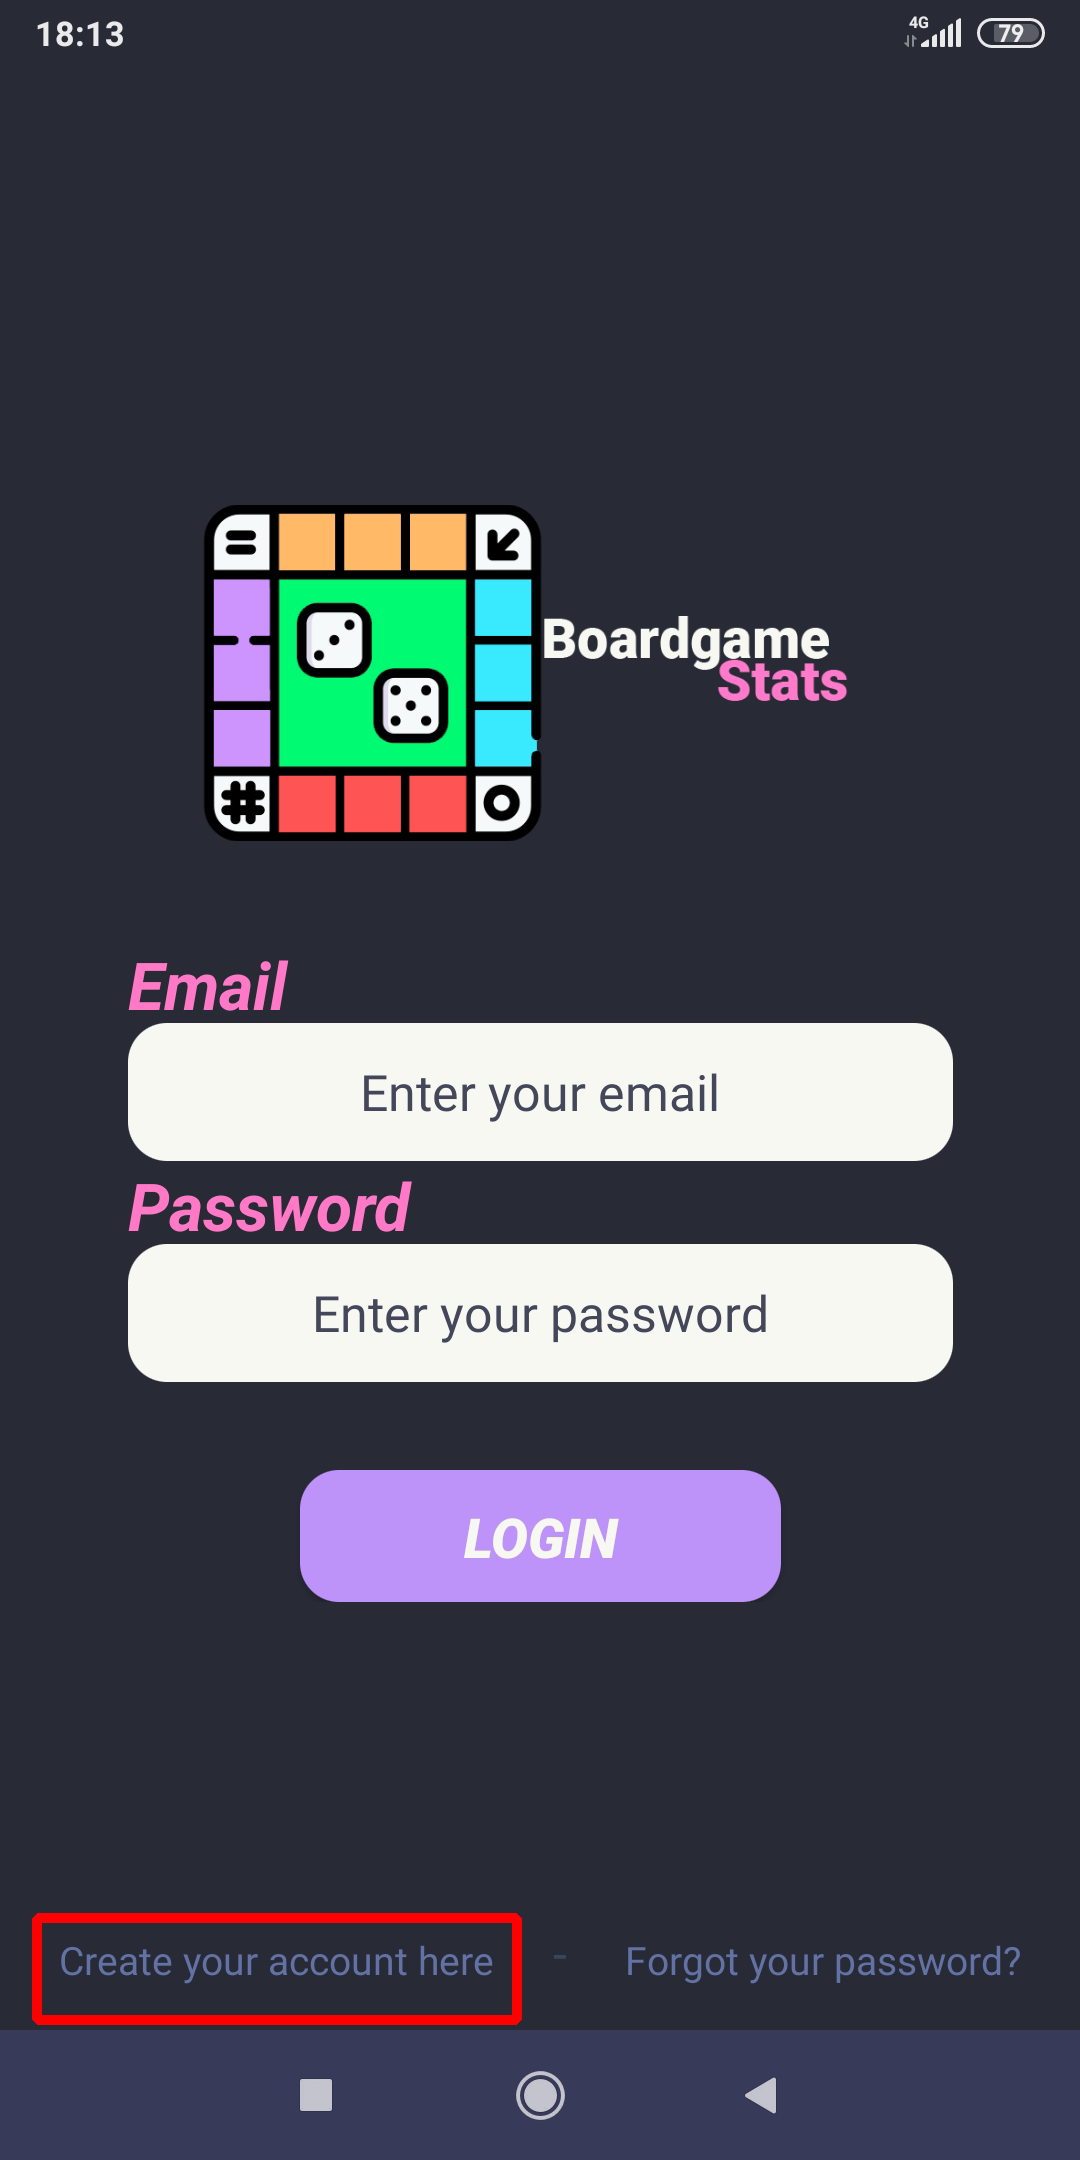
\includegraphics[width=0.3\linewidth]{fig/Uso/2.png}
    \caption{Iniciar registro}
    \label{fig:uso2}
\end{figure}

Una vez dentro de la actividad para registrarnos veremos algo como lo de ahora.

\begin{figure}[H]
    \centering
    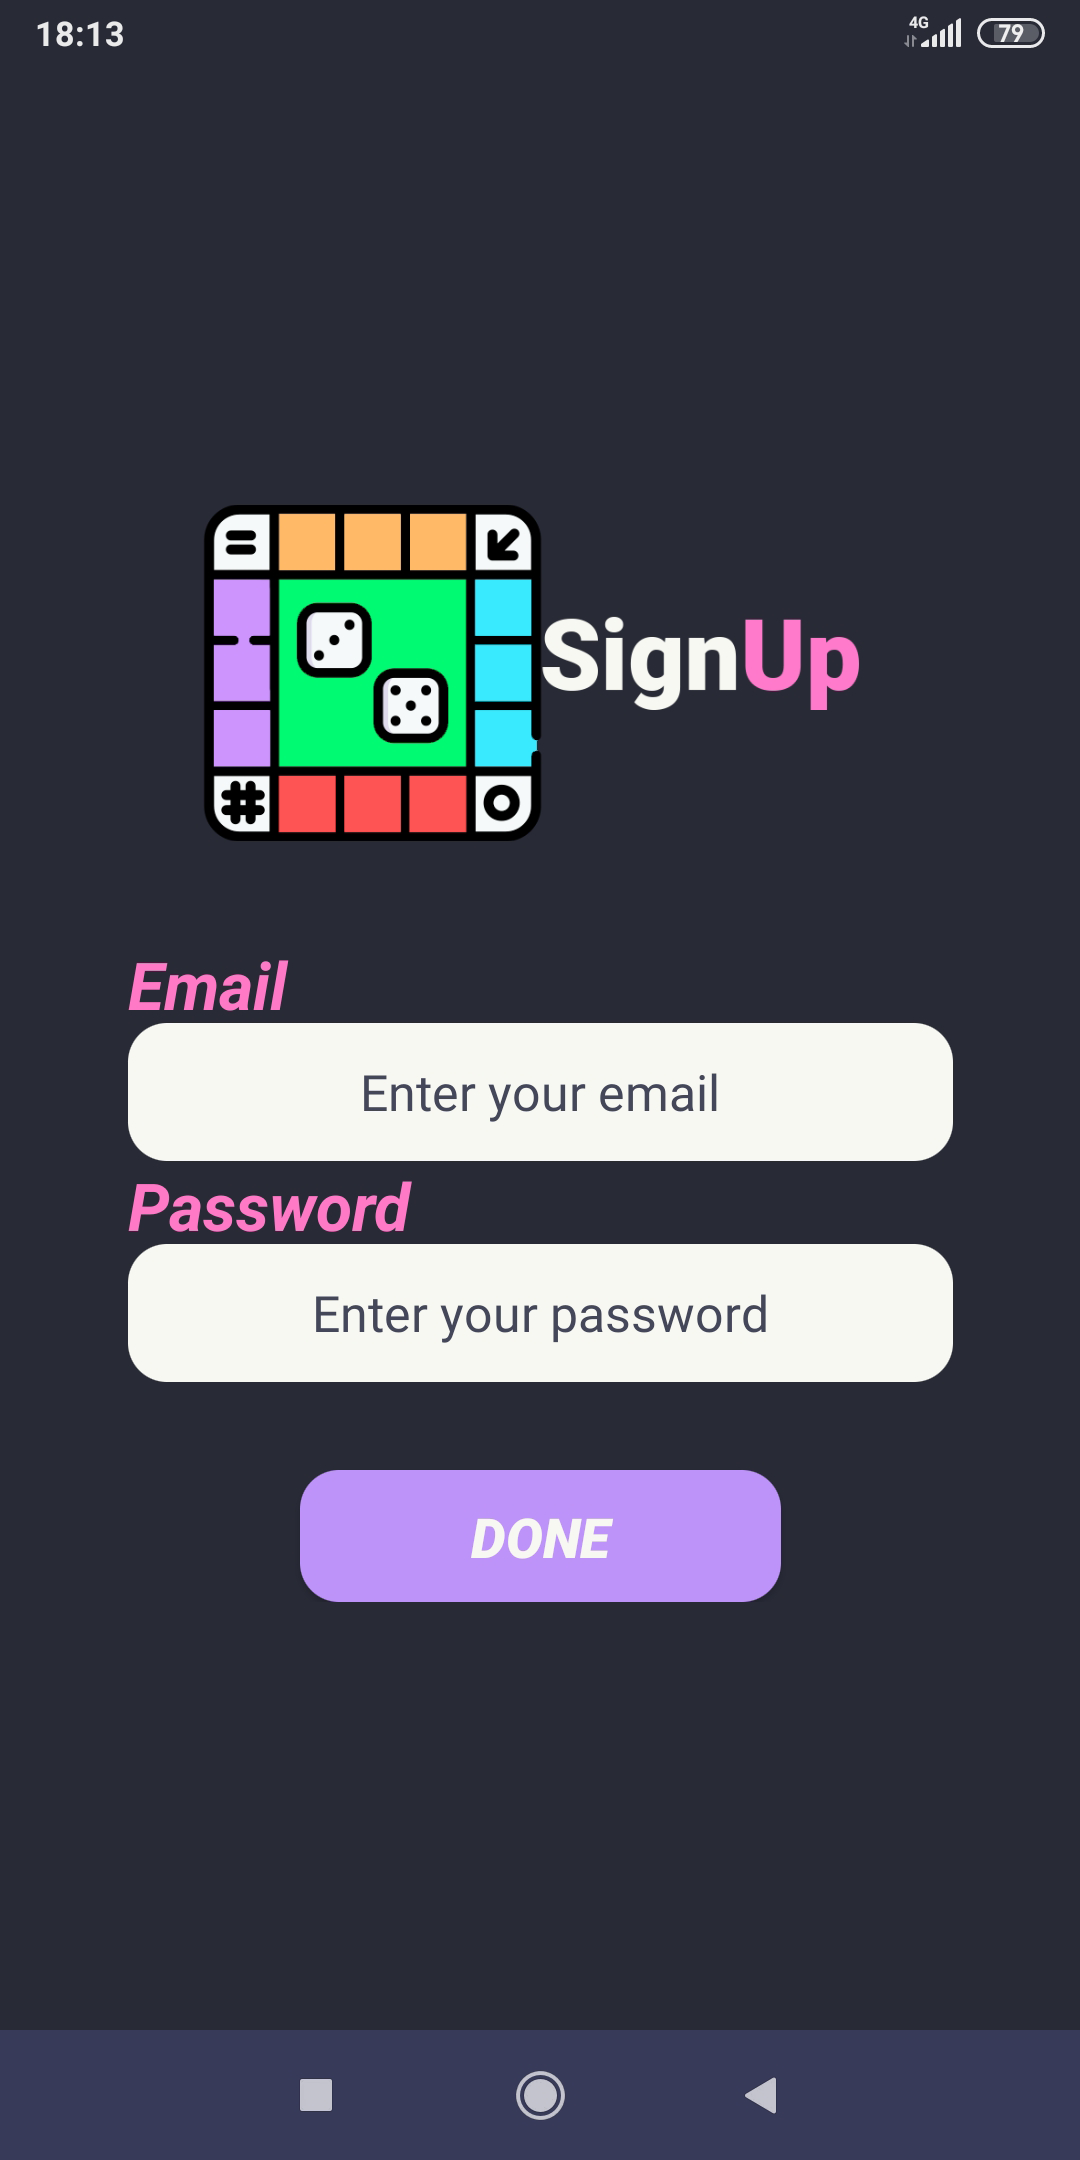
\includegraphics[width=0.3\linewidth]{fig/Uso/3.png}
    \caption{Registro}
    \label{fig:uso3}
\end{figure}

Donde tendremos que escibir nuestro correo y contraseña, y, por último, clicar en el botón que pone \textit{Done}.

\begin{figure}[H]
    \centering
    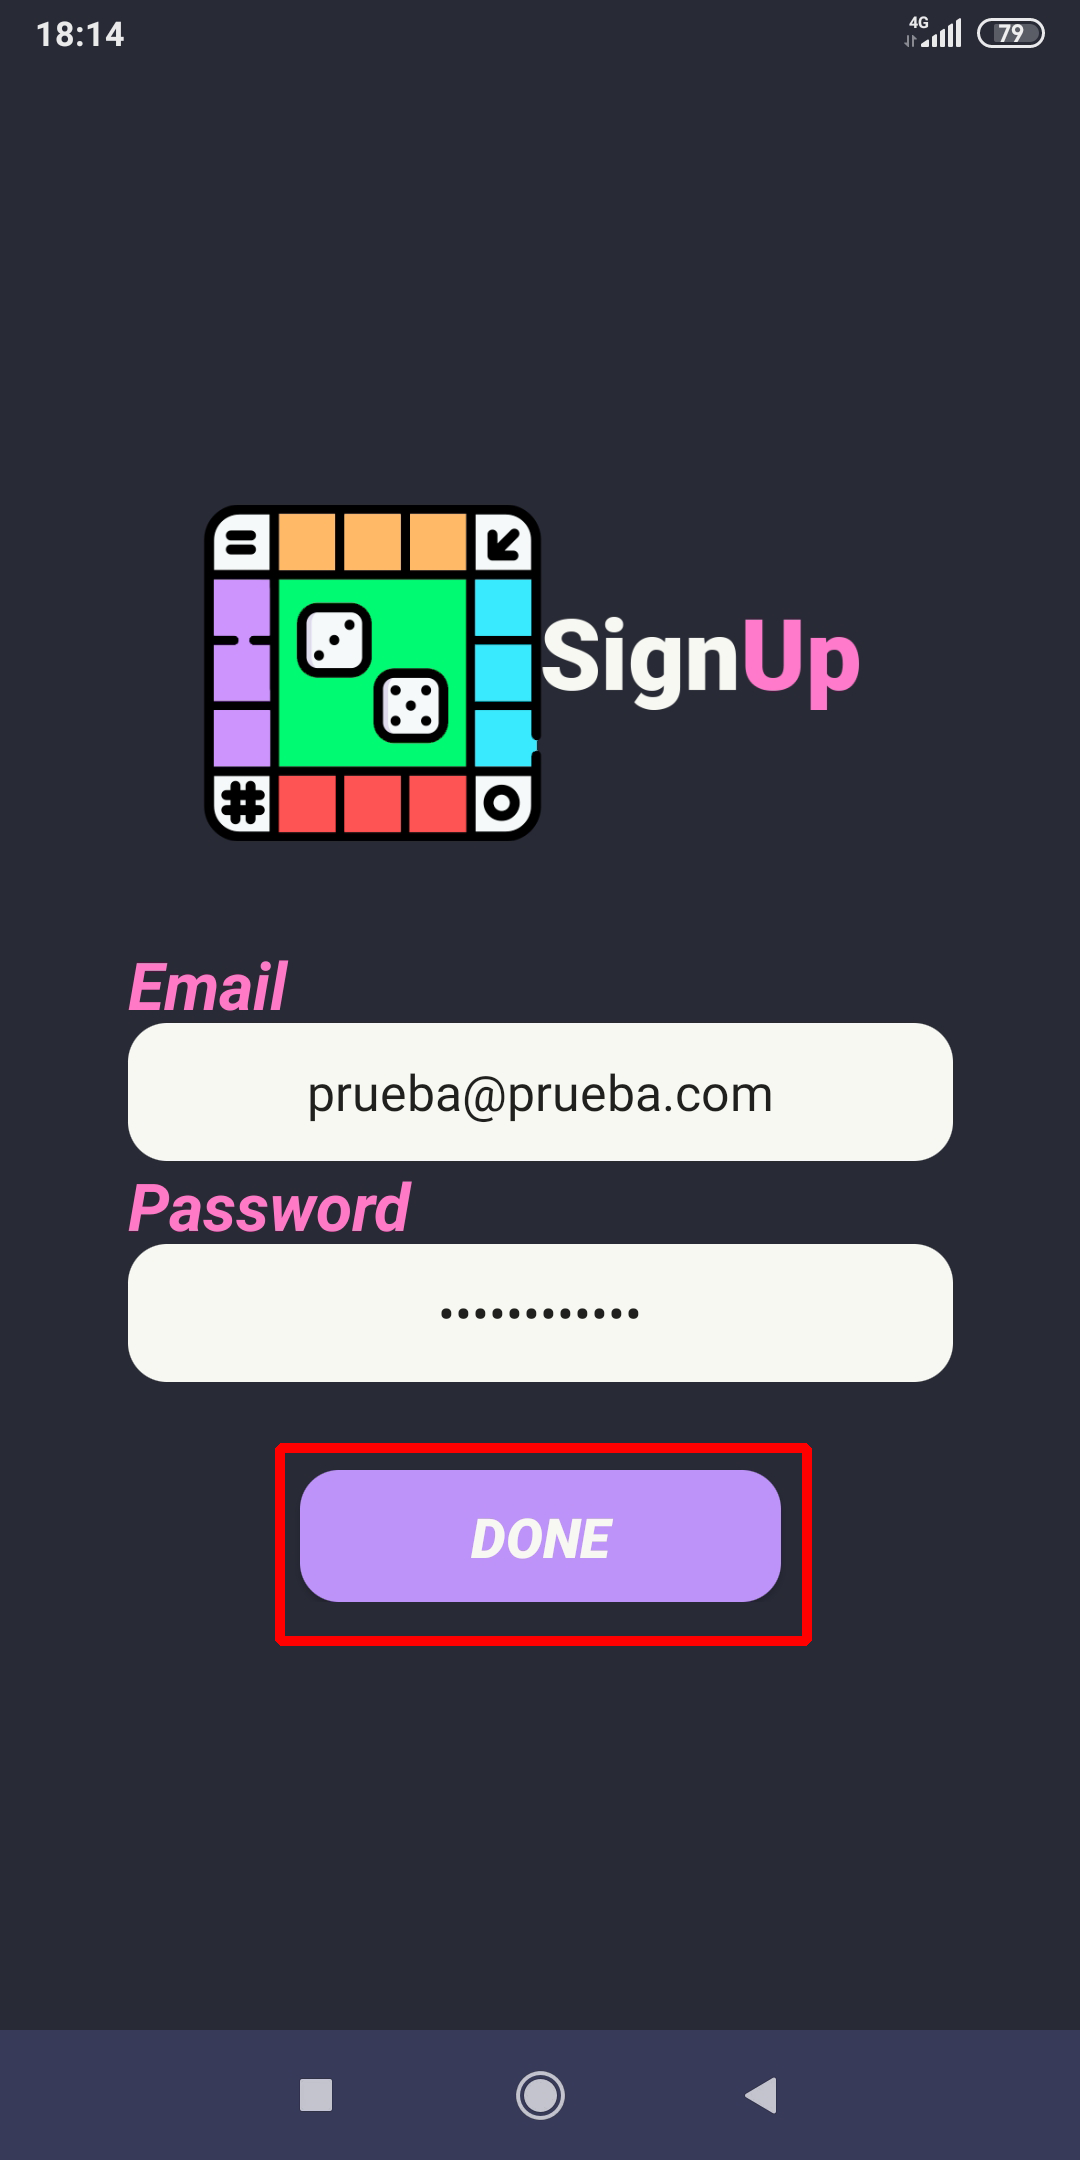
\includegraphics[width=0.3\linewidth]{fig/Uso/4.png}
    \caption{Completar registro}
    \label{fig:uso4}
\end{figure}

También, estando en la ventana de inicio de sesión, podremos clicar sobre el texto que pone \textit{Forgot your password?}, el cual nos abrirá el siguiente pop-up, donde podremos escribir nuestro correo electrónico para que nos haga llegar un correo para restablecer la contraseña.

\begin{figure}[H]
    \centering
    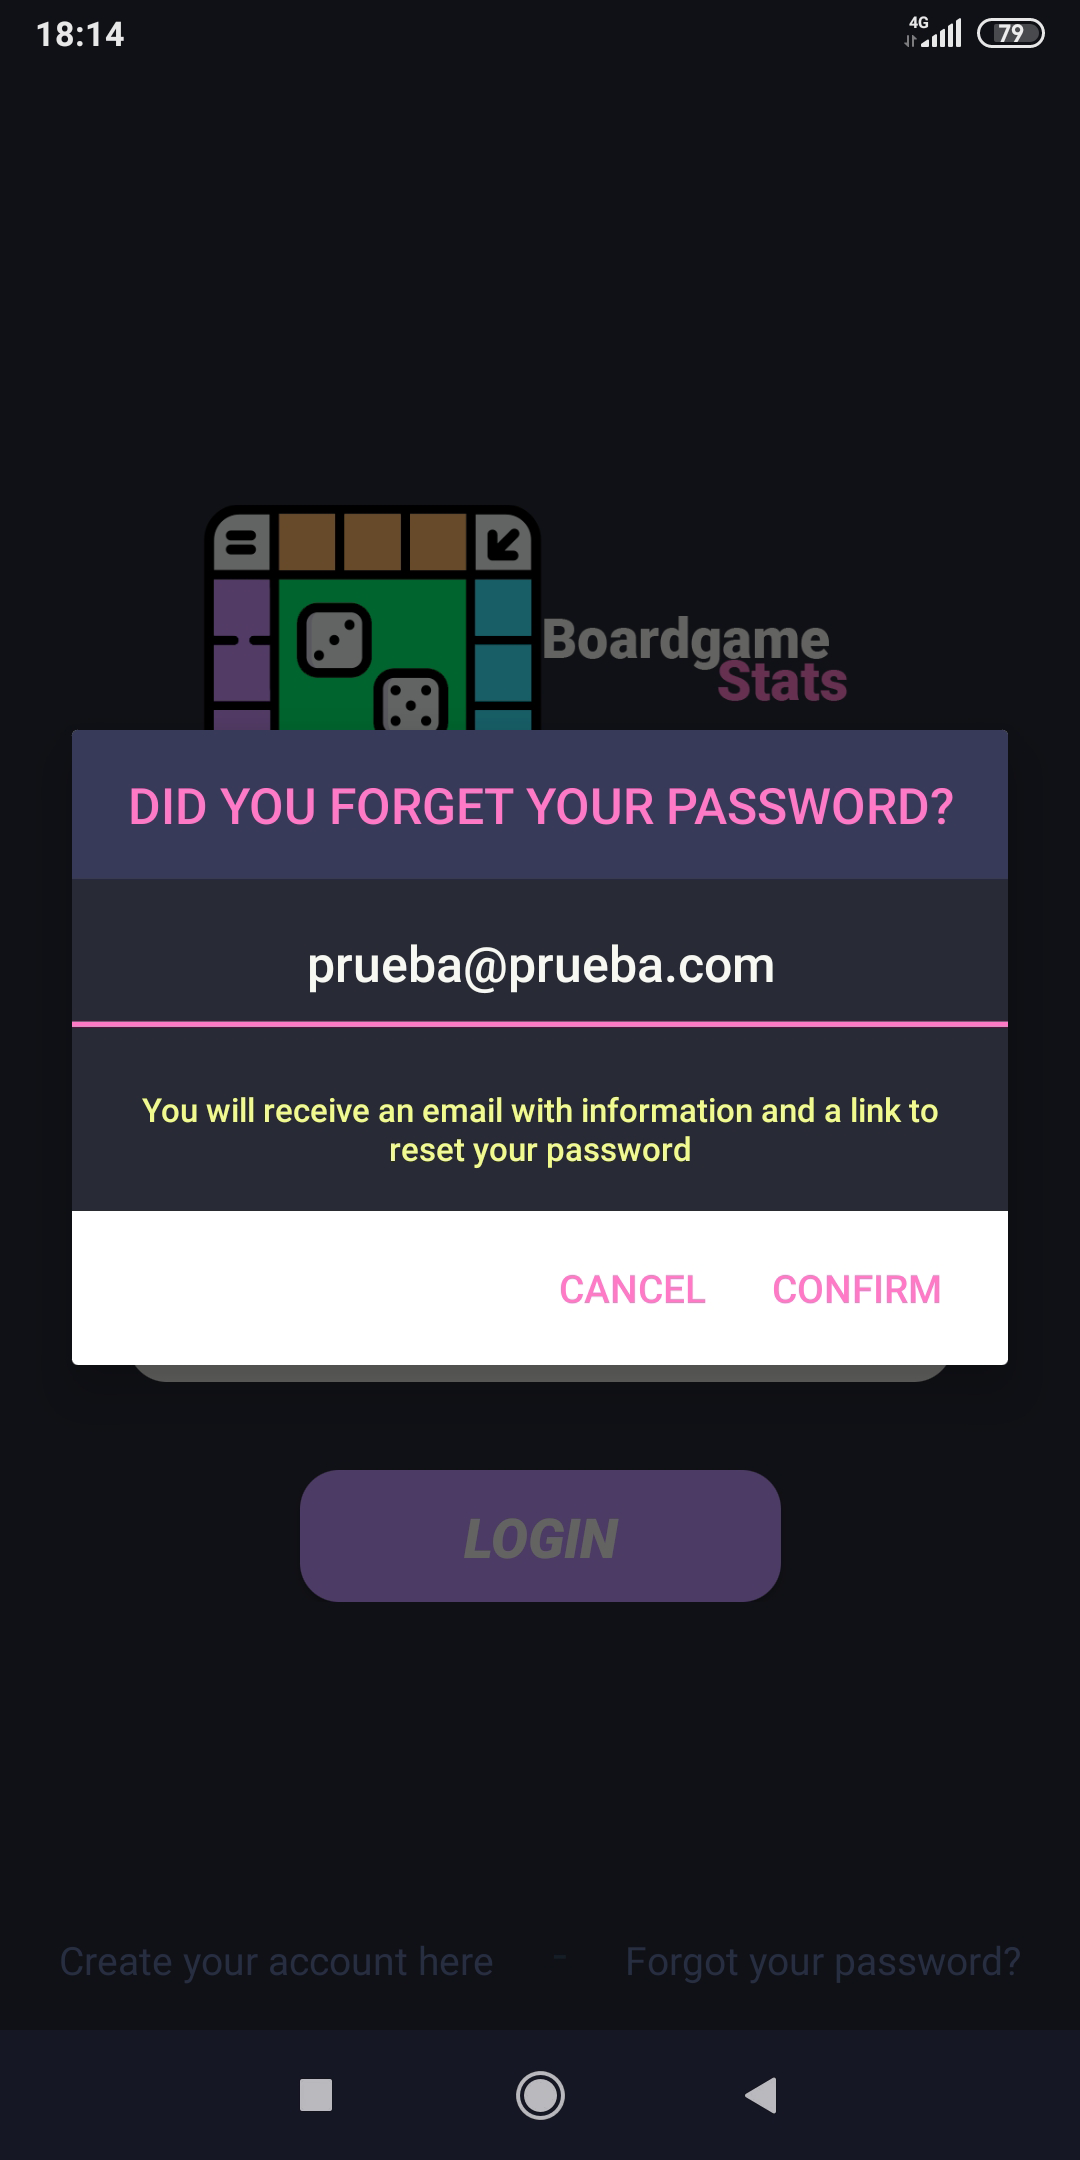
\includegraphics[width=0.3\linewidth]{fig/Uso/5.png}
    \caption{¿Olvidaste la contraseña?}
    \label{fig:uso5}
\end{figure}

Una vez estemos ya registrados, usaremos dicha cuenta para iniciar sesión en la aplicación.

\begin{figure}[H]
    \centering
    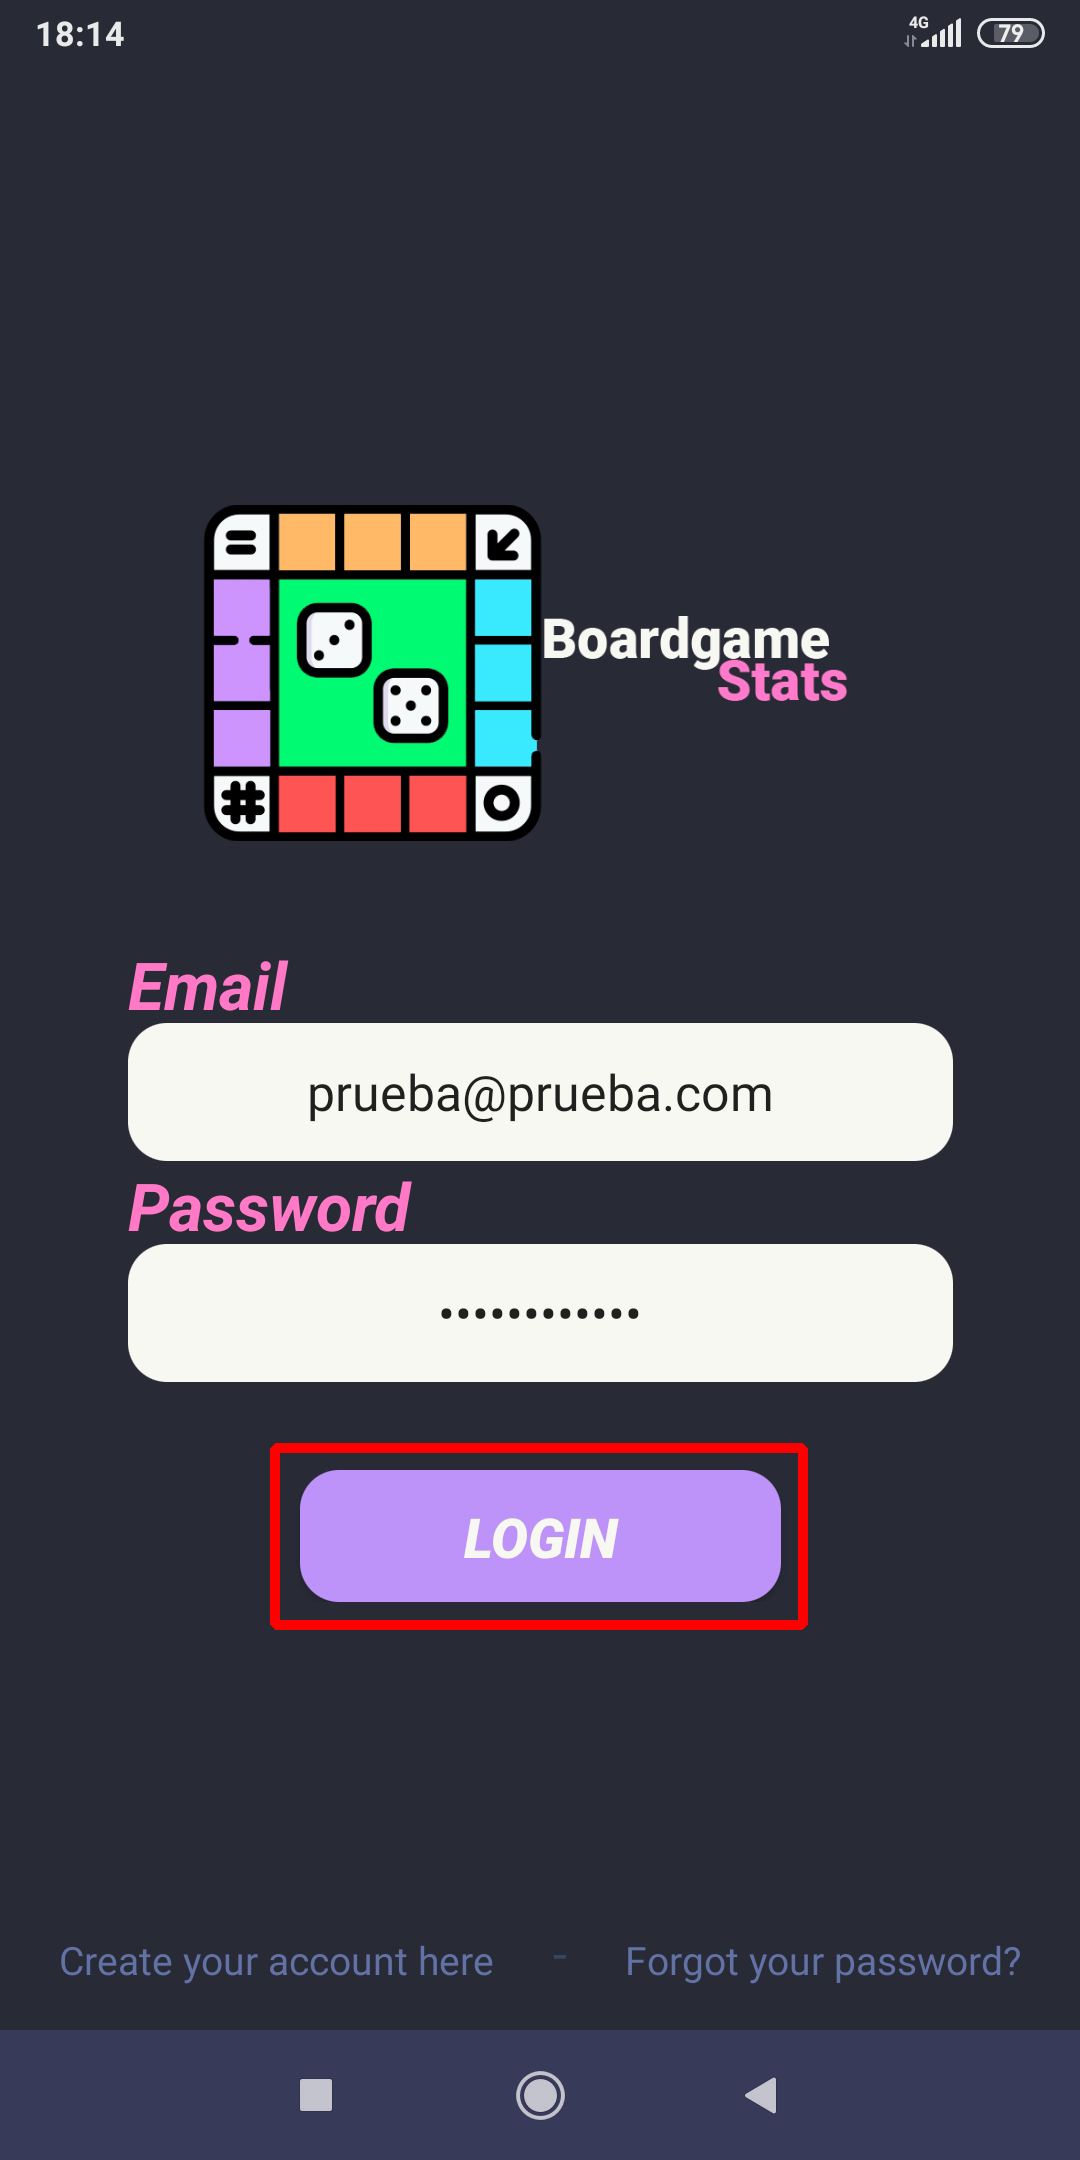
\includegraphics[width=0.3\linewidth]{fig/Uso/6.png}
    \caption{Inicio sesión completado}
    \label{fig:uso6}
\end{figure}

Con la sesión ya iniciada, lo primero que veremos será esta ventana en la que tendremos una lista vacía o con juegos que vayamos seleccionando de uno en uno, un texto con el que accederemos a la actividad para seleccionar dichos juegos, y una barra de navegación en la zona inferior de la ventana.

\begin{figure}[H]
    \centering
    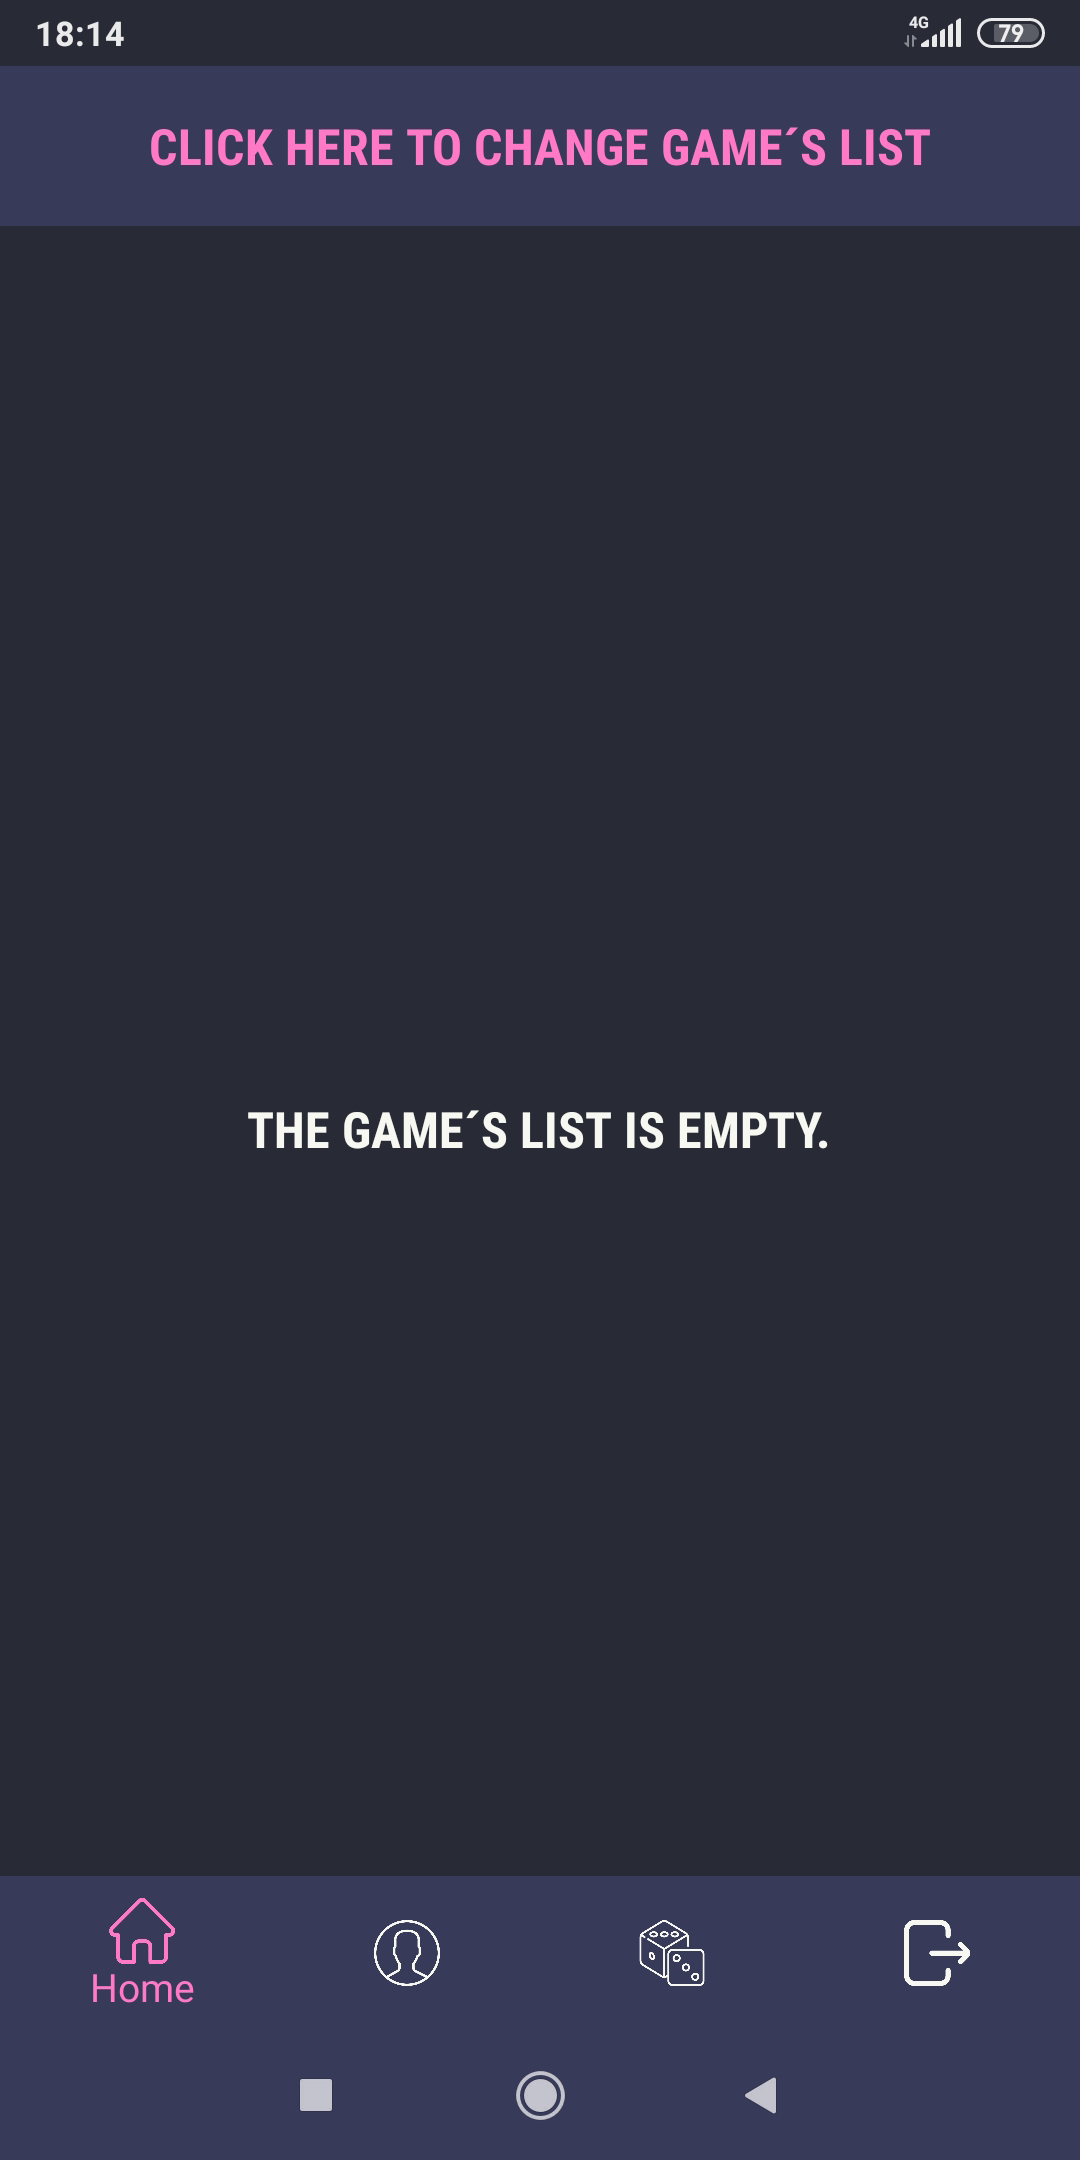
\includegraphics[width=0.3\linewidth]{fig/Uso/7.png}
    \caption{Actividad Home con lista vacía}
    \label{fig:uso7}
\end{figure}

\begin{figure}[H]
    \centering
    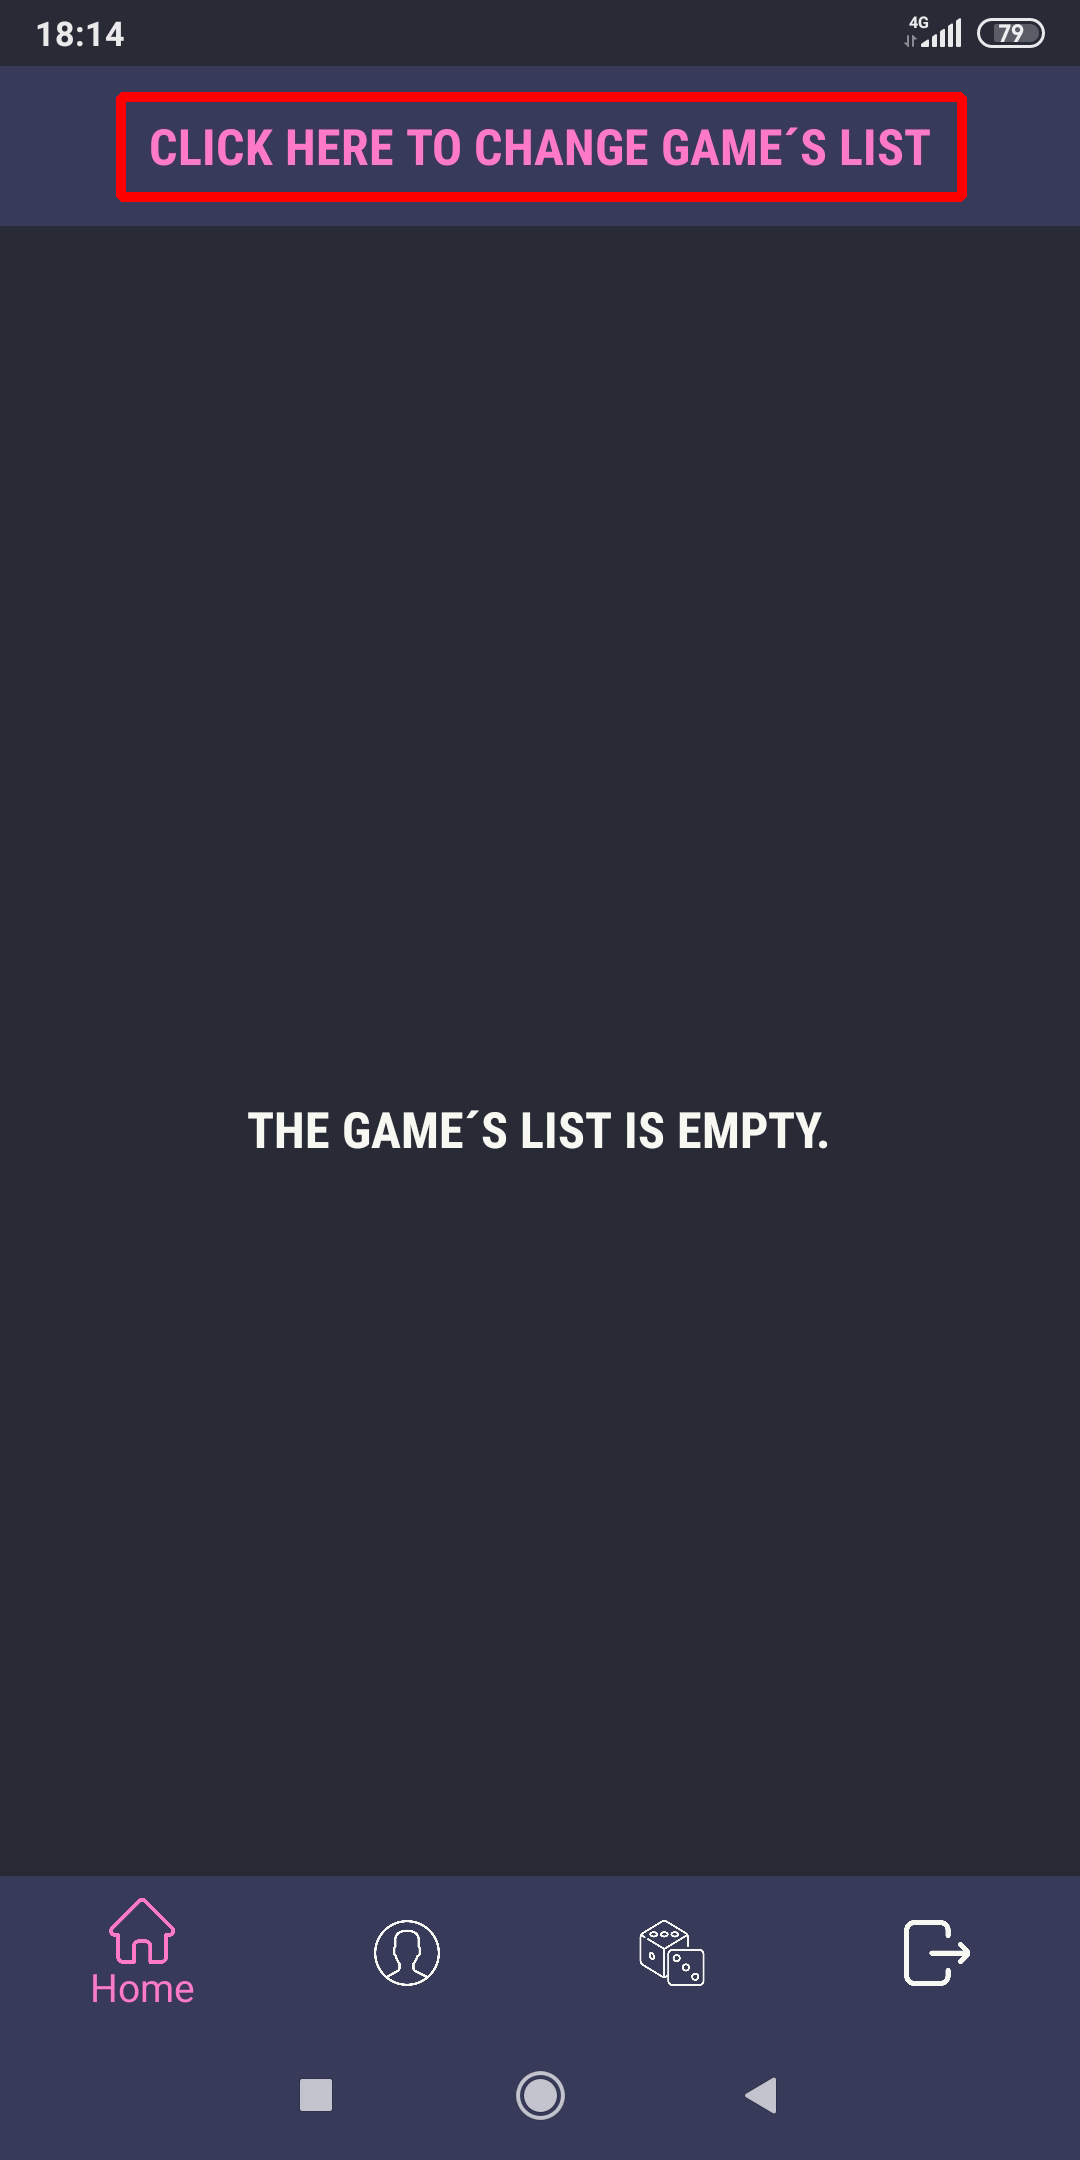
\includegraphics[width=0.3\linewidth]{fig/Uso/8.png}
    \caption{Texto para seleccionar juegos}
    \label{fig:uso8}
\end{figure}

\begin{figure}[H]
    \centering
    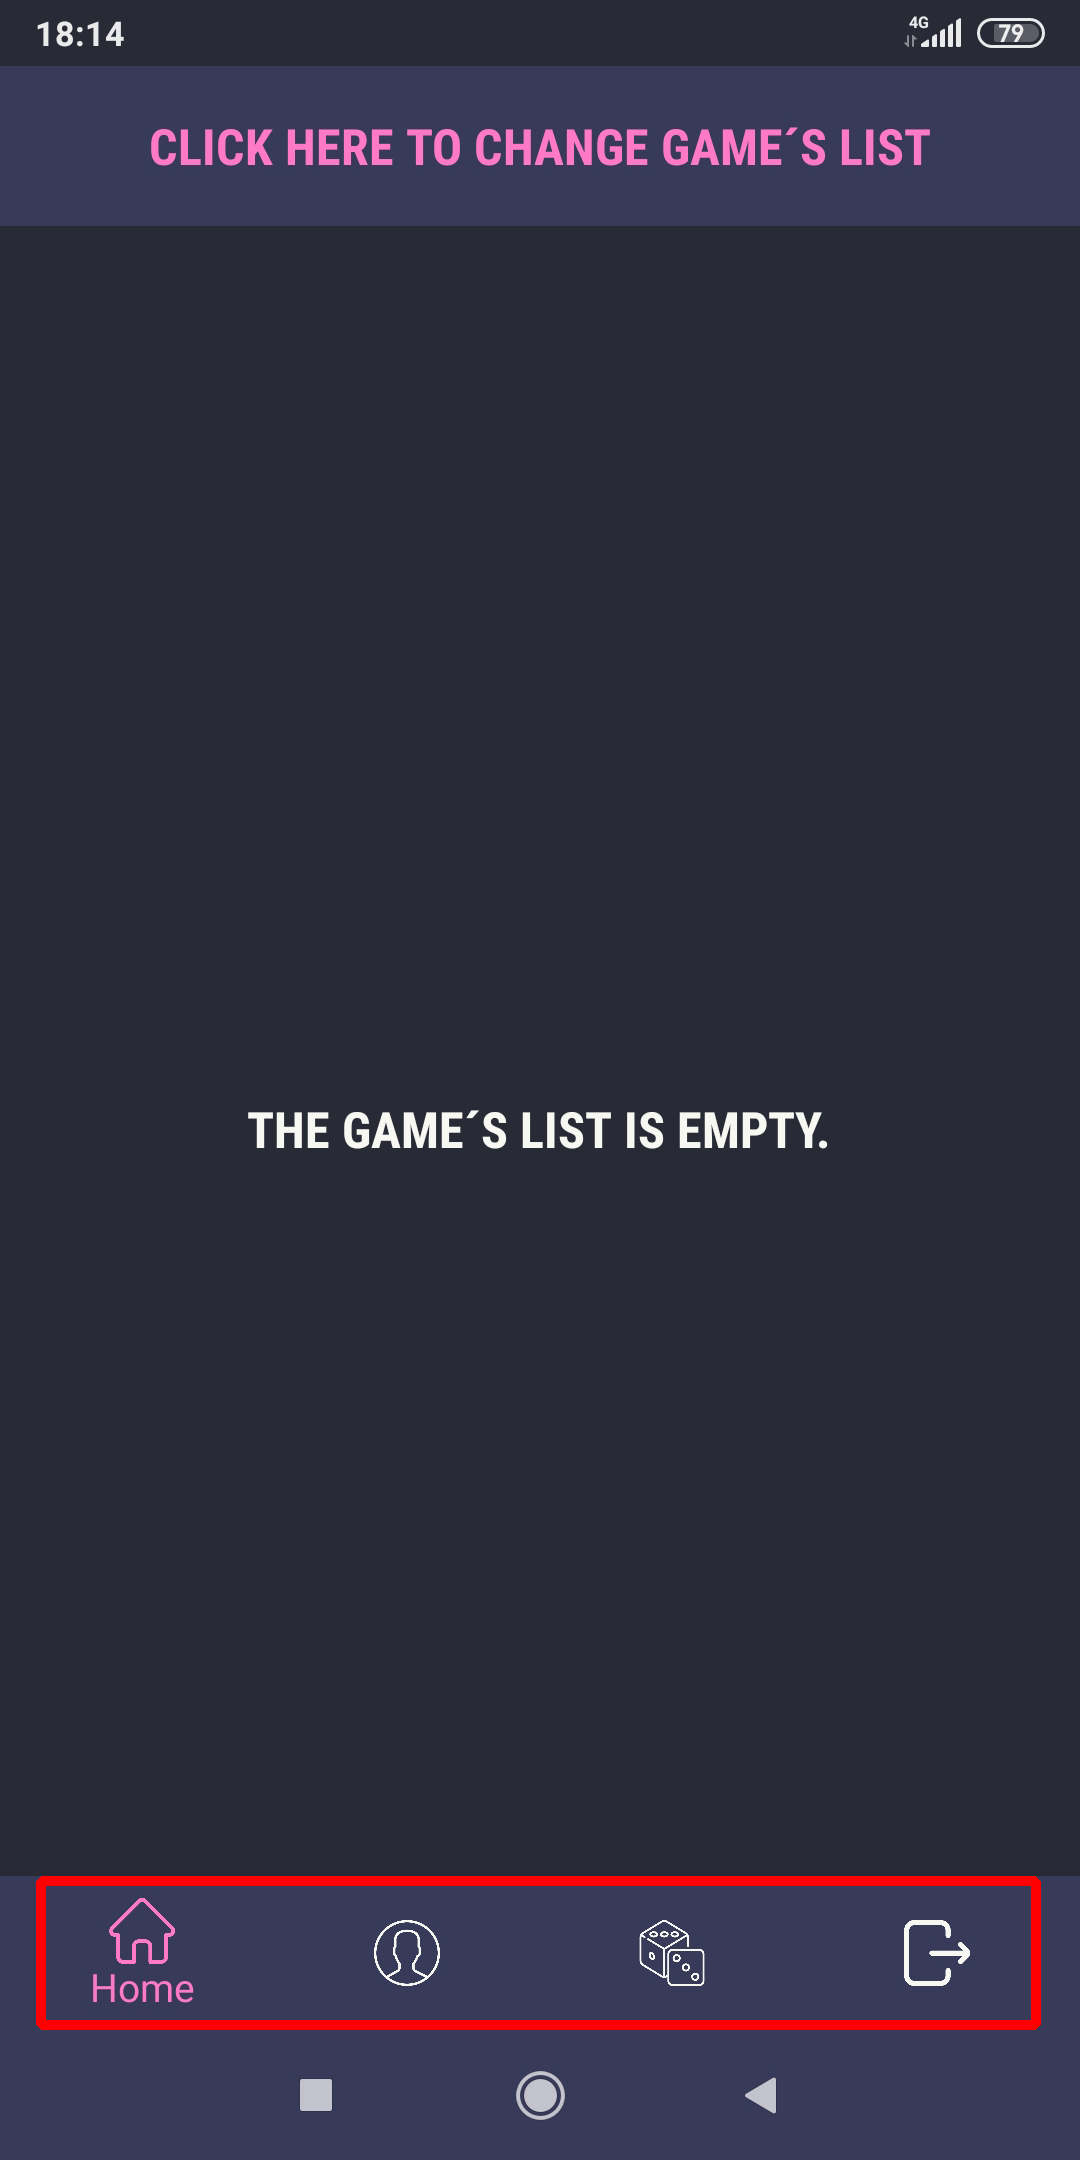
\includegraphics[width=0.3\linewidth]{fig/Uso/9.png}
    \caption{Barra de navegación}
    \label{fig:uso9}
\end{figure}

Si entramos en la actividad para seleccionar juegos, nos encontraremos con una barra de búsqueda

\begin{figure}[H]
    \centering
    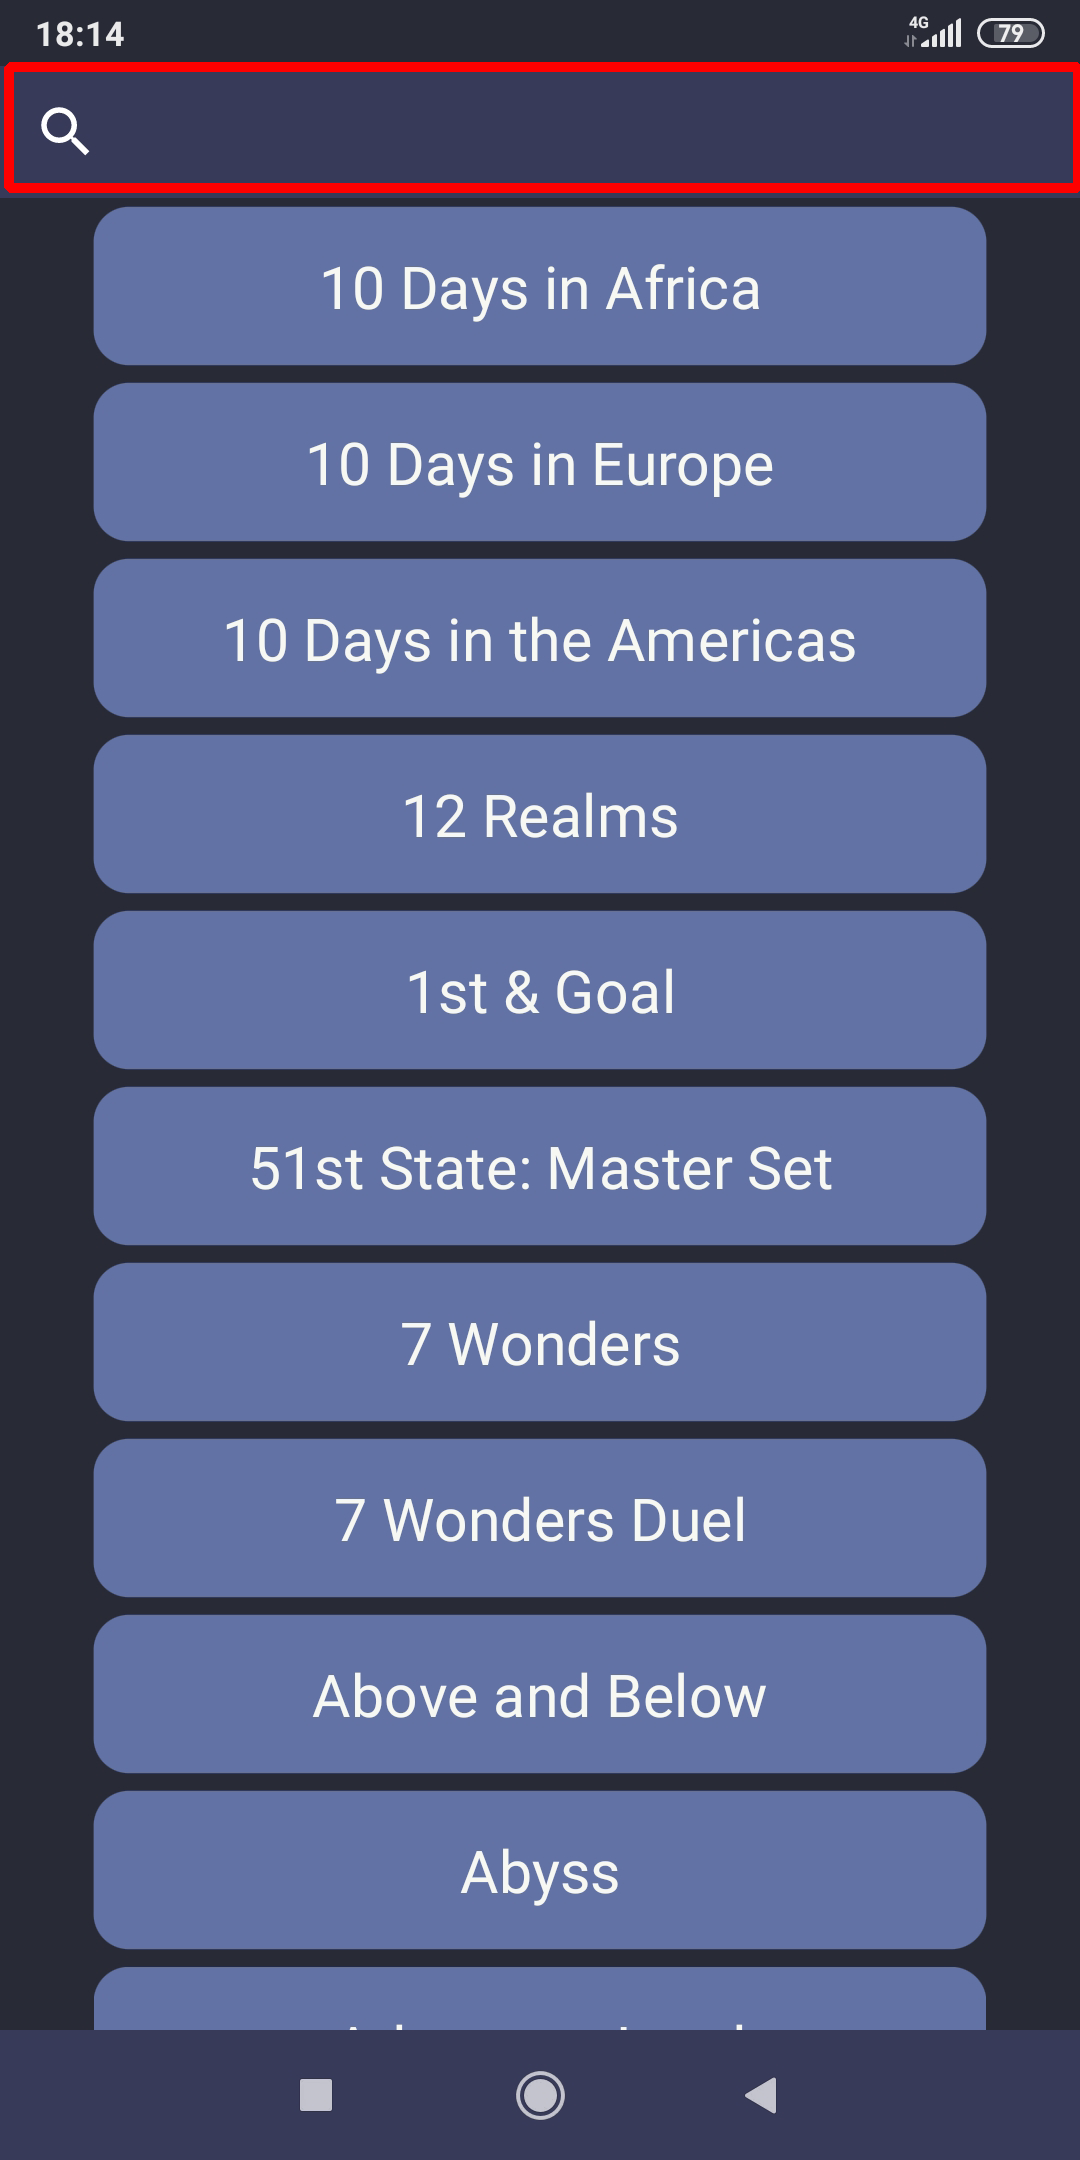
\includegraphics[width=0.3\linewidth]{fig/Uso/10.png}
    \caption{Barra de búsqueda de juegos}
    \label{fig:uso10}
\end{figure}

y una lista rellena de juegos de mesa sacados de una API en la que se puede hacer scroll.

\begin{figure}[H]
    \centering
    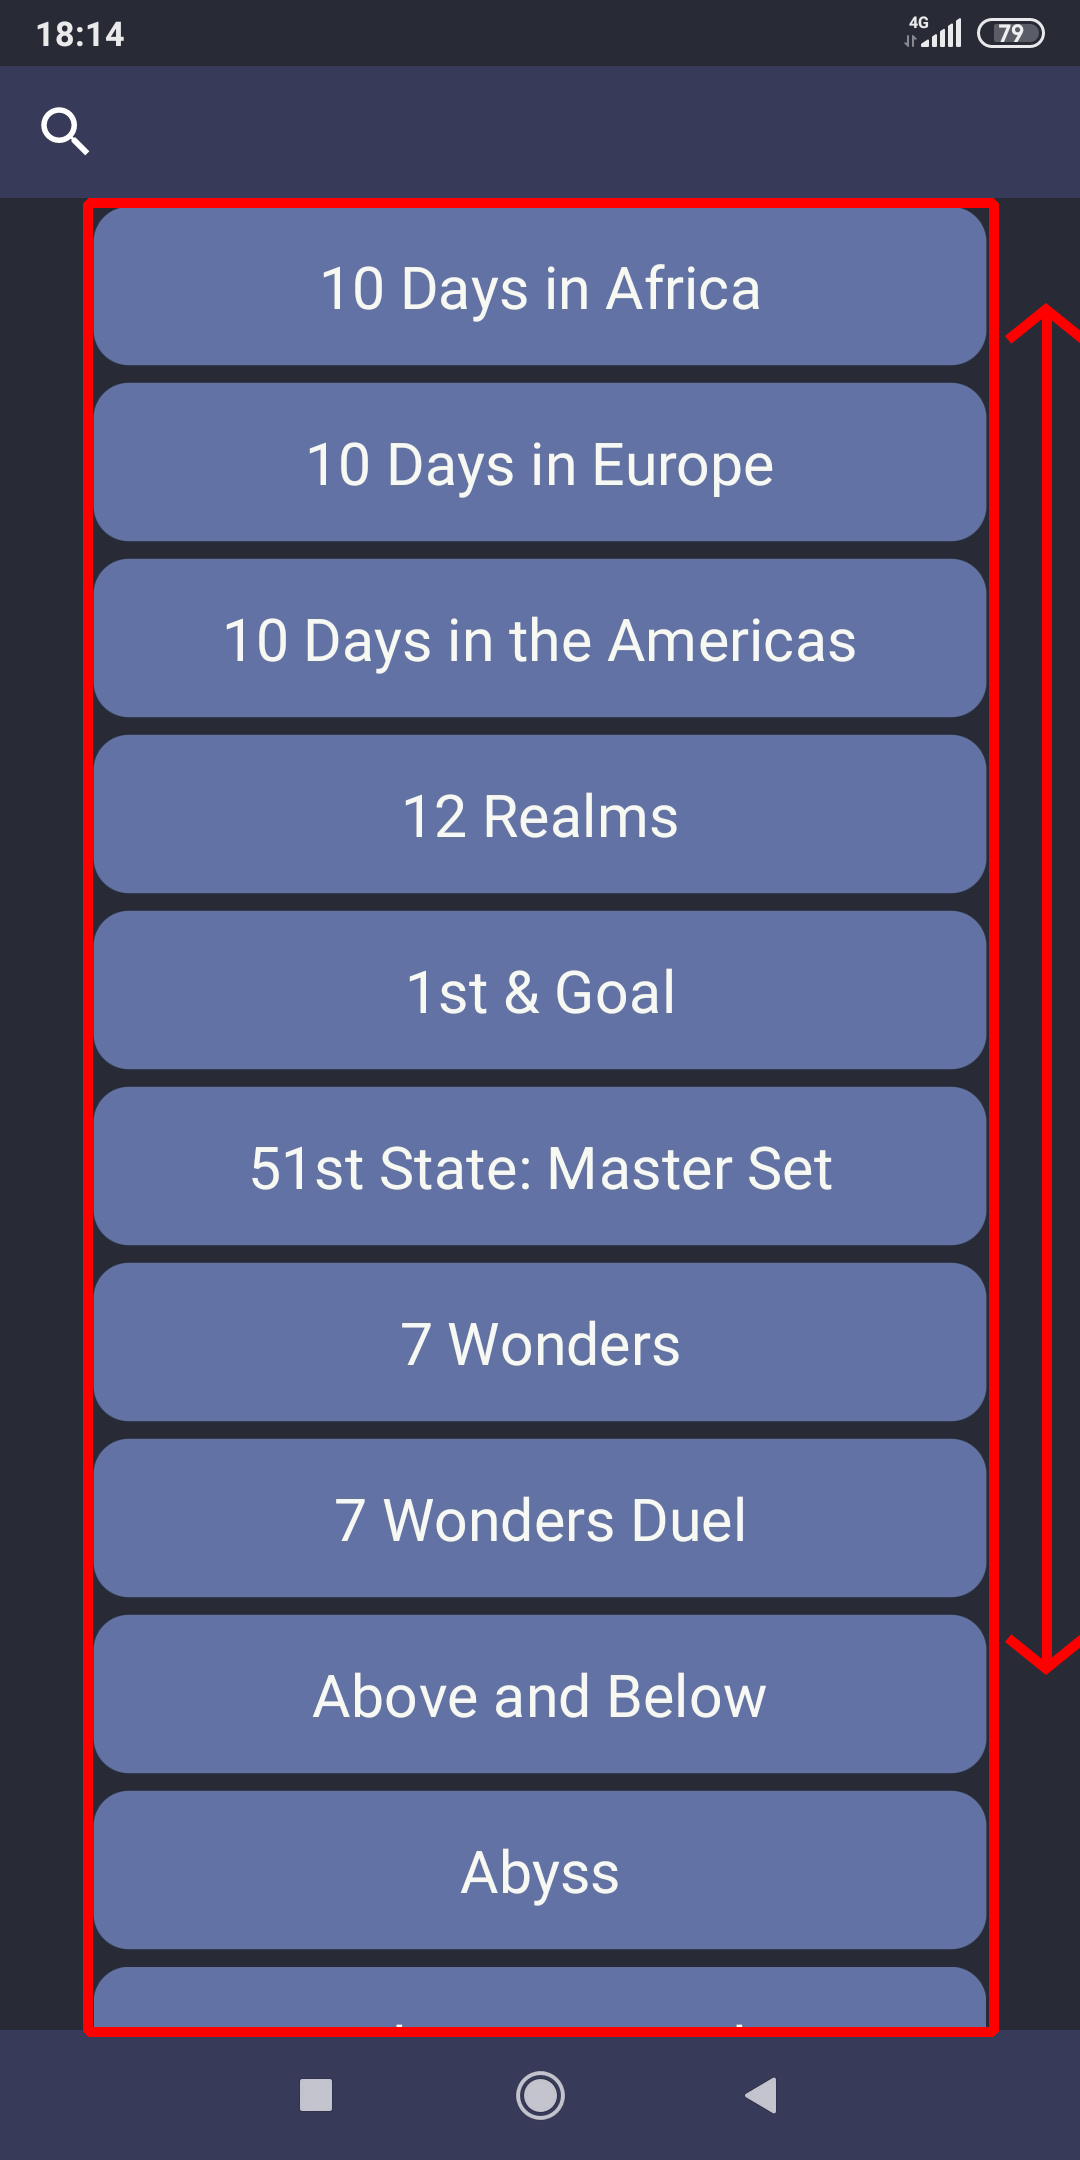
\includegraphics[width=0.3\linewidth]{fig/Uso/11.png}
    \caption{Lista de juegos completa}
    \label{fig:uso11}
\end{figure}

Cuando seleccionamos un juego de esta lista, veremos las estadísticas que tengamos en ese juego de mesa y un botón con el que podremos agregar dicho juego a nuestra lista de juegos favoritos haciendo que aparezca en la lista de la actividad principal y un mensaje notificándonos de esto.

\begin{figure}[H]
    \centering
    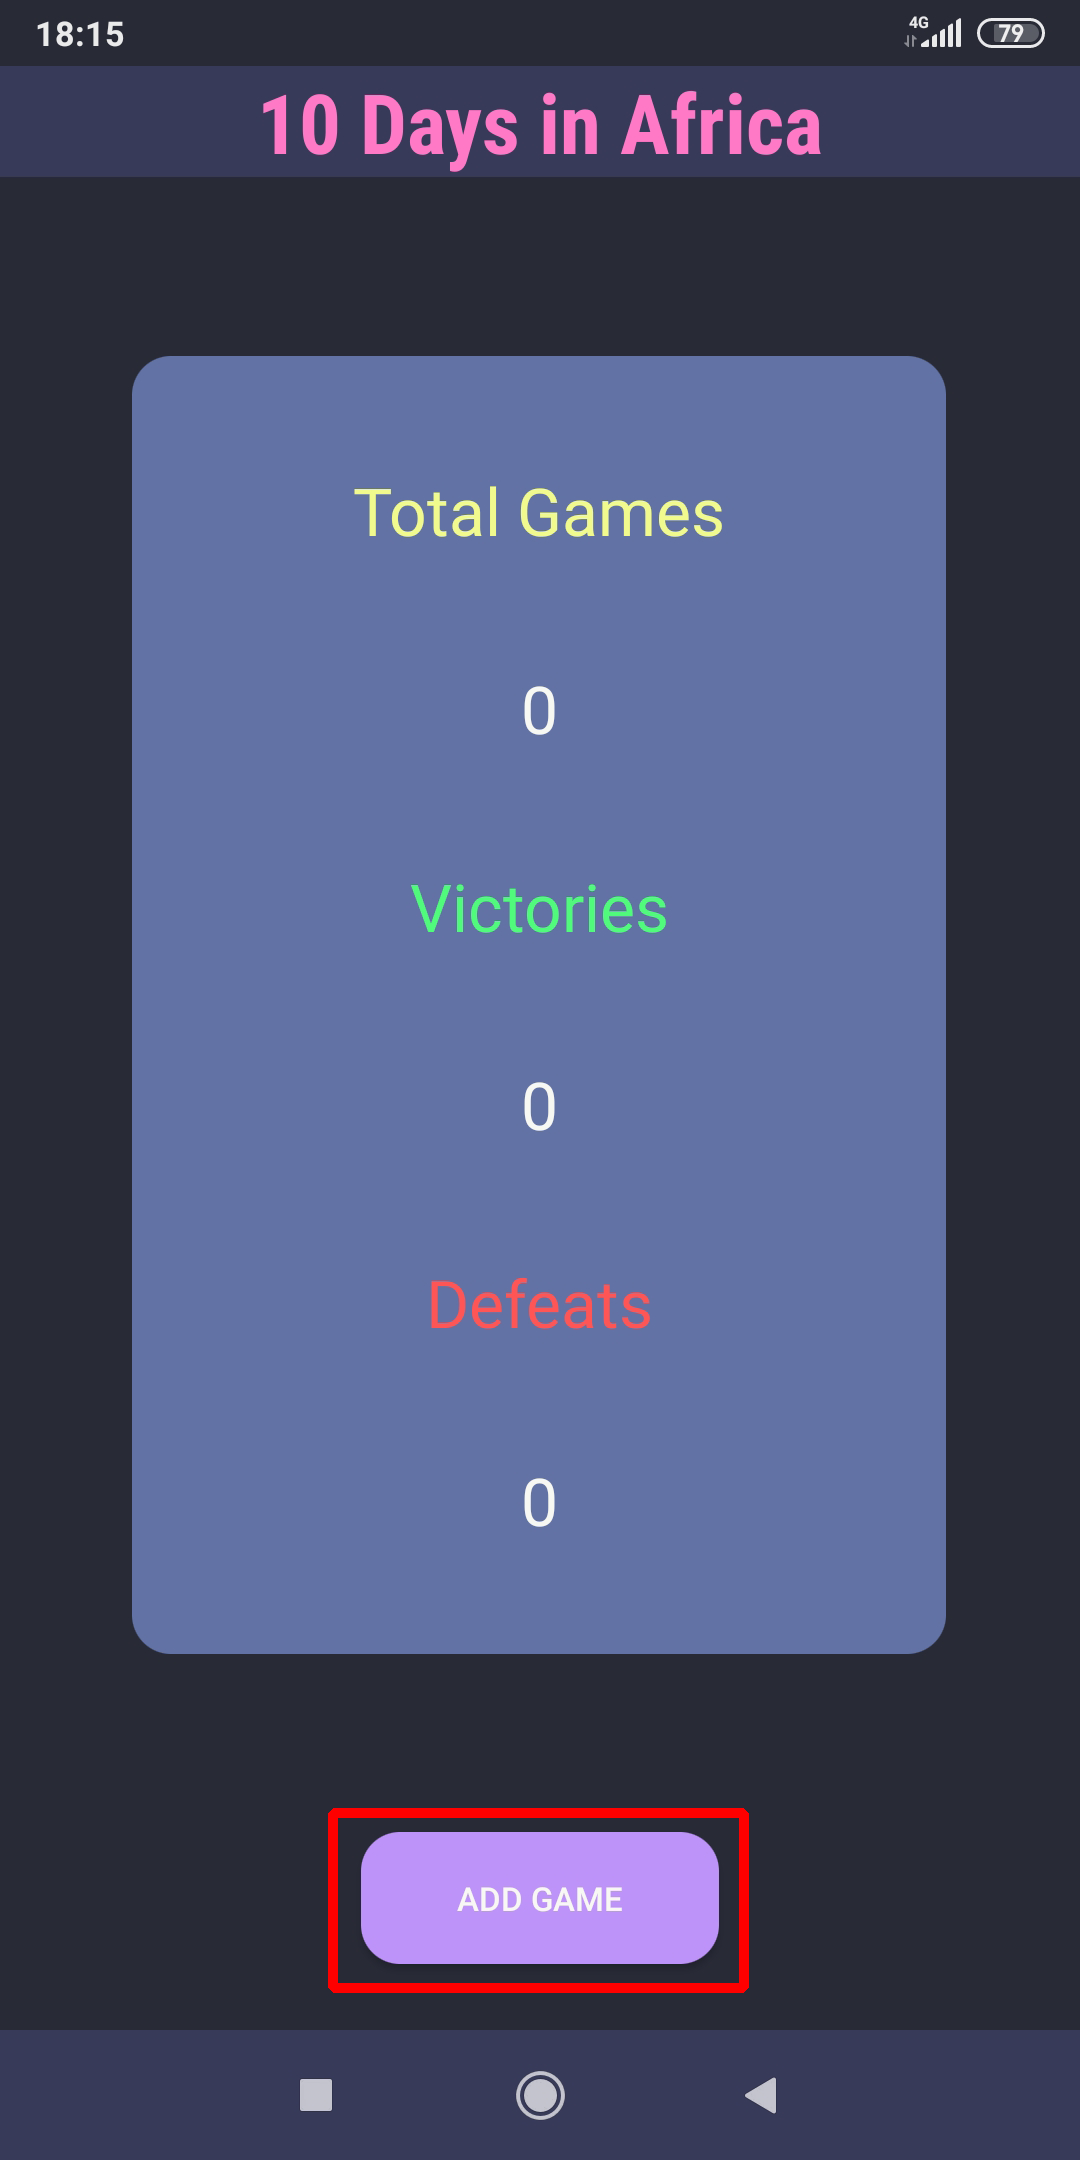
\includegraphics[width=0.3\linewidth]{fig/Uso/12.png}
    \caption{Añadir juego a lista de juegos favoritos}
    \label{fig:uso12}
\end{figure}

\begin{figure}[H]
    \centering
    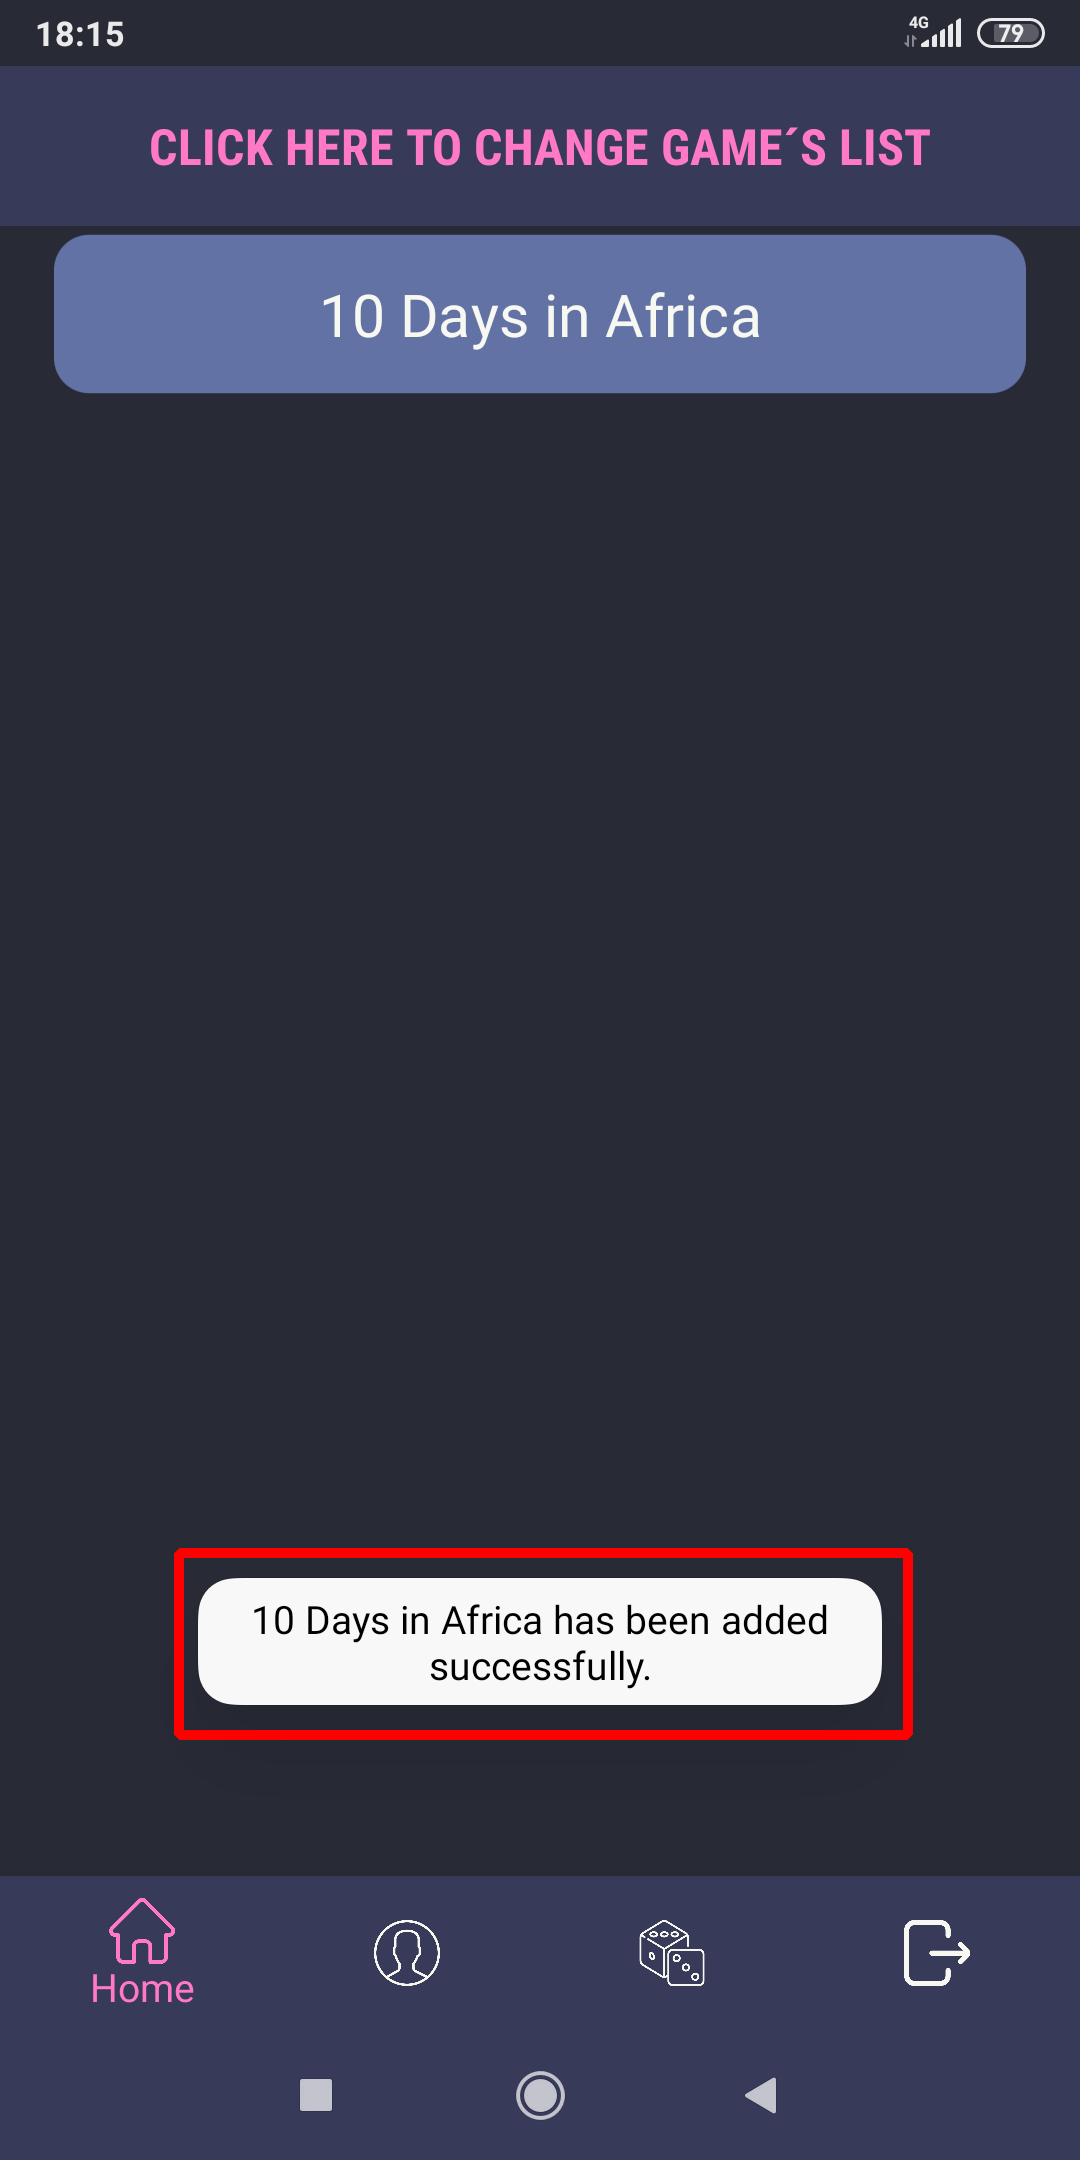
\includegraphics[width=0.3\linewidth]{fig/Uso/13.png}
    \caption{Notificación de que un juego ha sido añadido}
    \label{fig:uso13}
\end{figure}

Aclarar que la lista de juegos favoritos también tiene la capacidad de hacer scroll.

\begin{figure}[H]
    \centering
    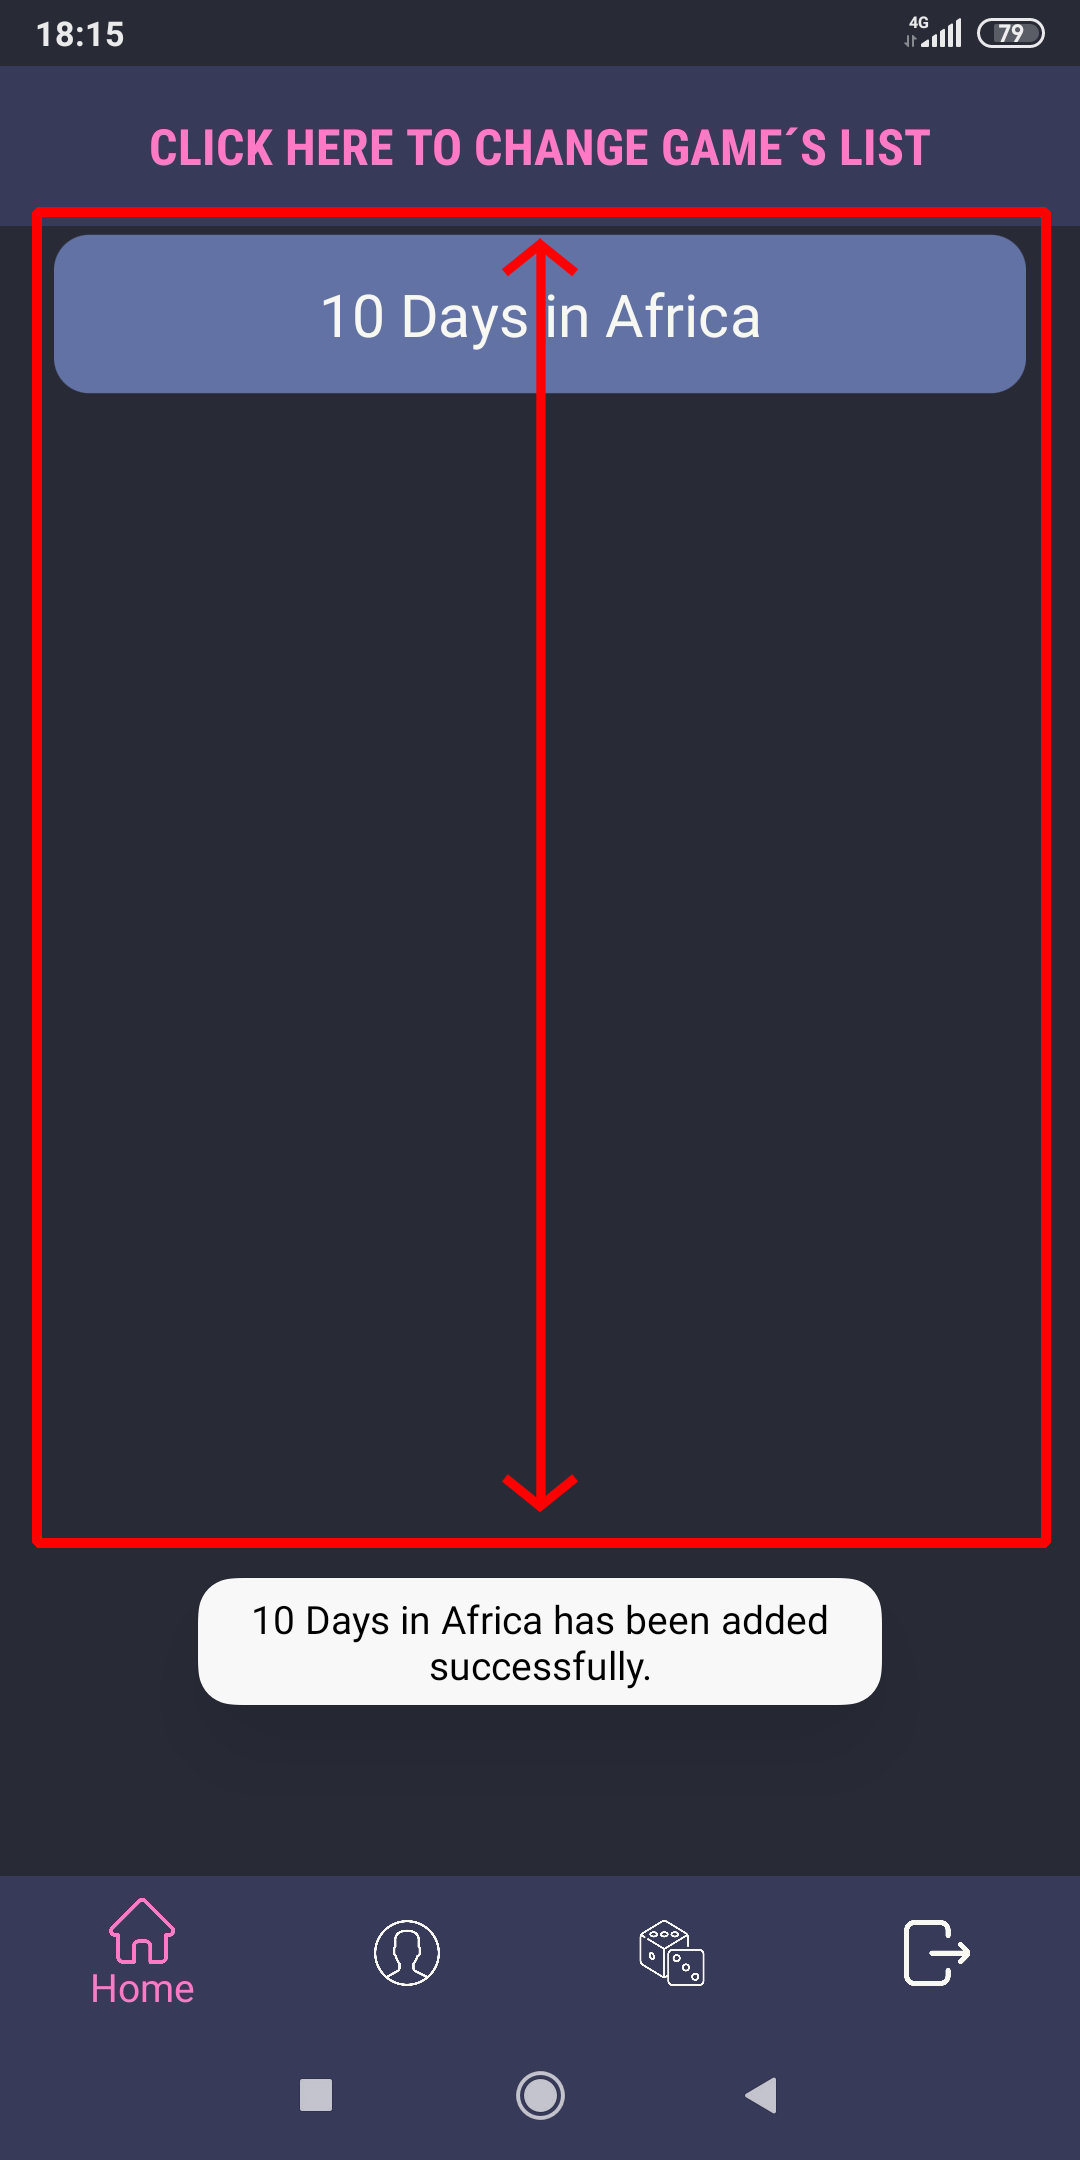
\includegraphics[width=0.3\linewidth]{fig/Uso/14.png}
    \caption{Scroll de lista de juegos favoritos}
    \label{fig:uso14}
\end{figure}

Cuando hacemos clic sobre uno de los juegos de esta lista, también nos abrirá una ventana con las estadísticas de este juego, pero con la diferencia de que ahora tendremos tres botones, en vez de uno único.

El primer botón que nos encontraremos será el que nos permita añadir partidas del juego seleccionado.

\begin{figure}[H]
    \centering
    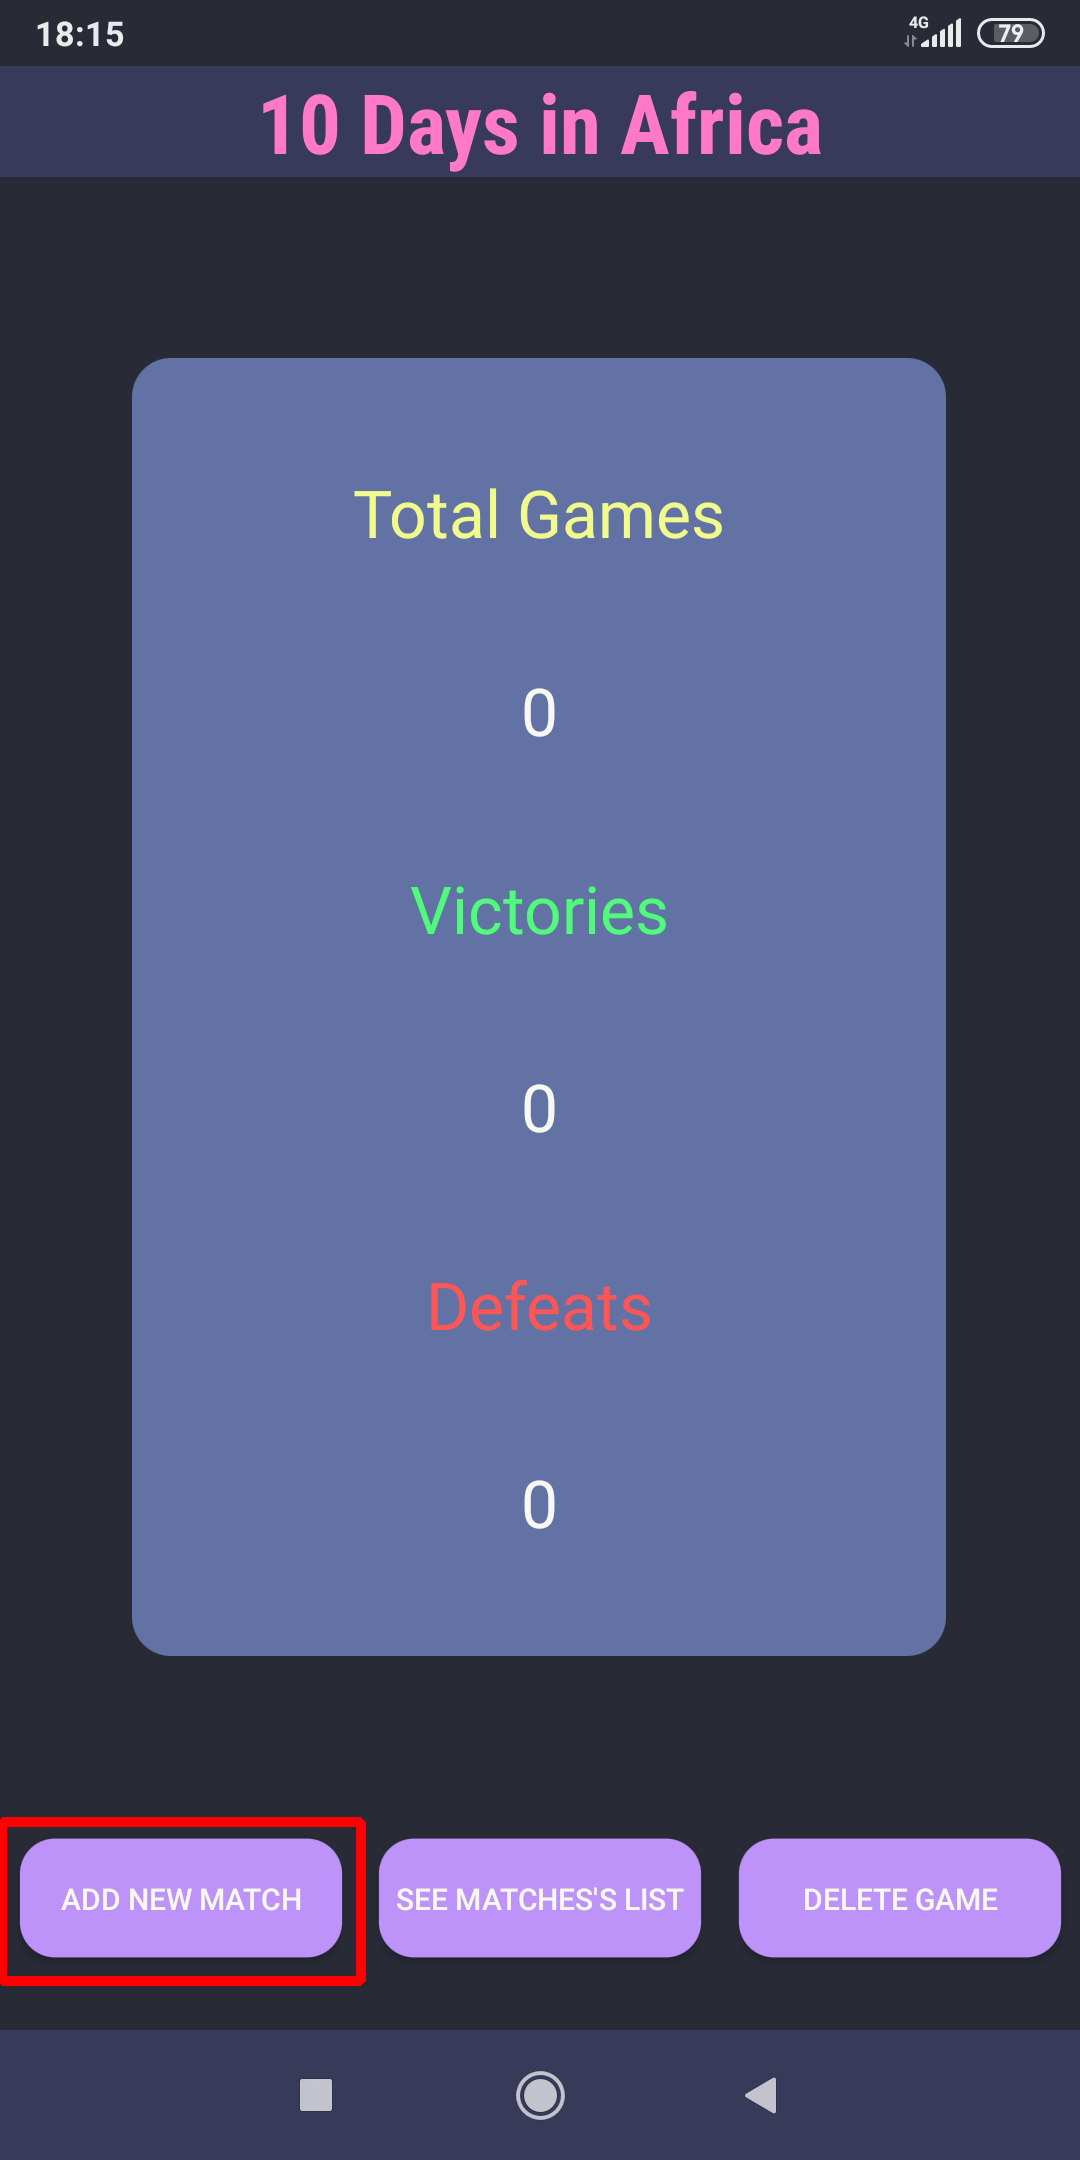
\includegraphics[width=0.3\linewidth]{fig/Uso/15.png}
    \caption{Botón para añadir partidas}
    \label{fig:uso15}
\end{figure}

Este botón nos abrirá la siguiente ventana en la que podremos escribir los nombres y las puntuaciones de hasta 8 jugadores.

Las puntuaciones serán añadidas a cada usuario y se le asignará una victoria o derrota dependiendo de su puntuación de forma automática.

\begin{figure}[H]
    \centering
    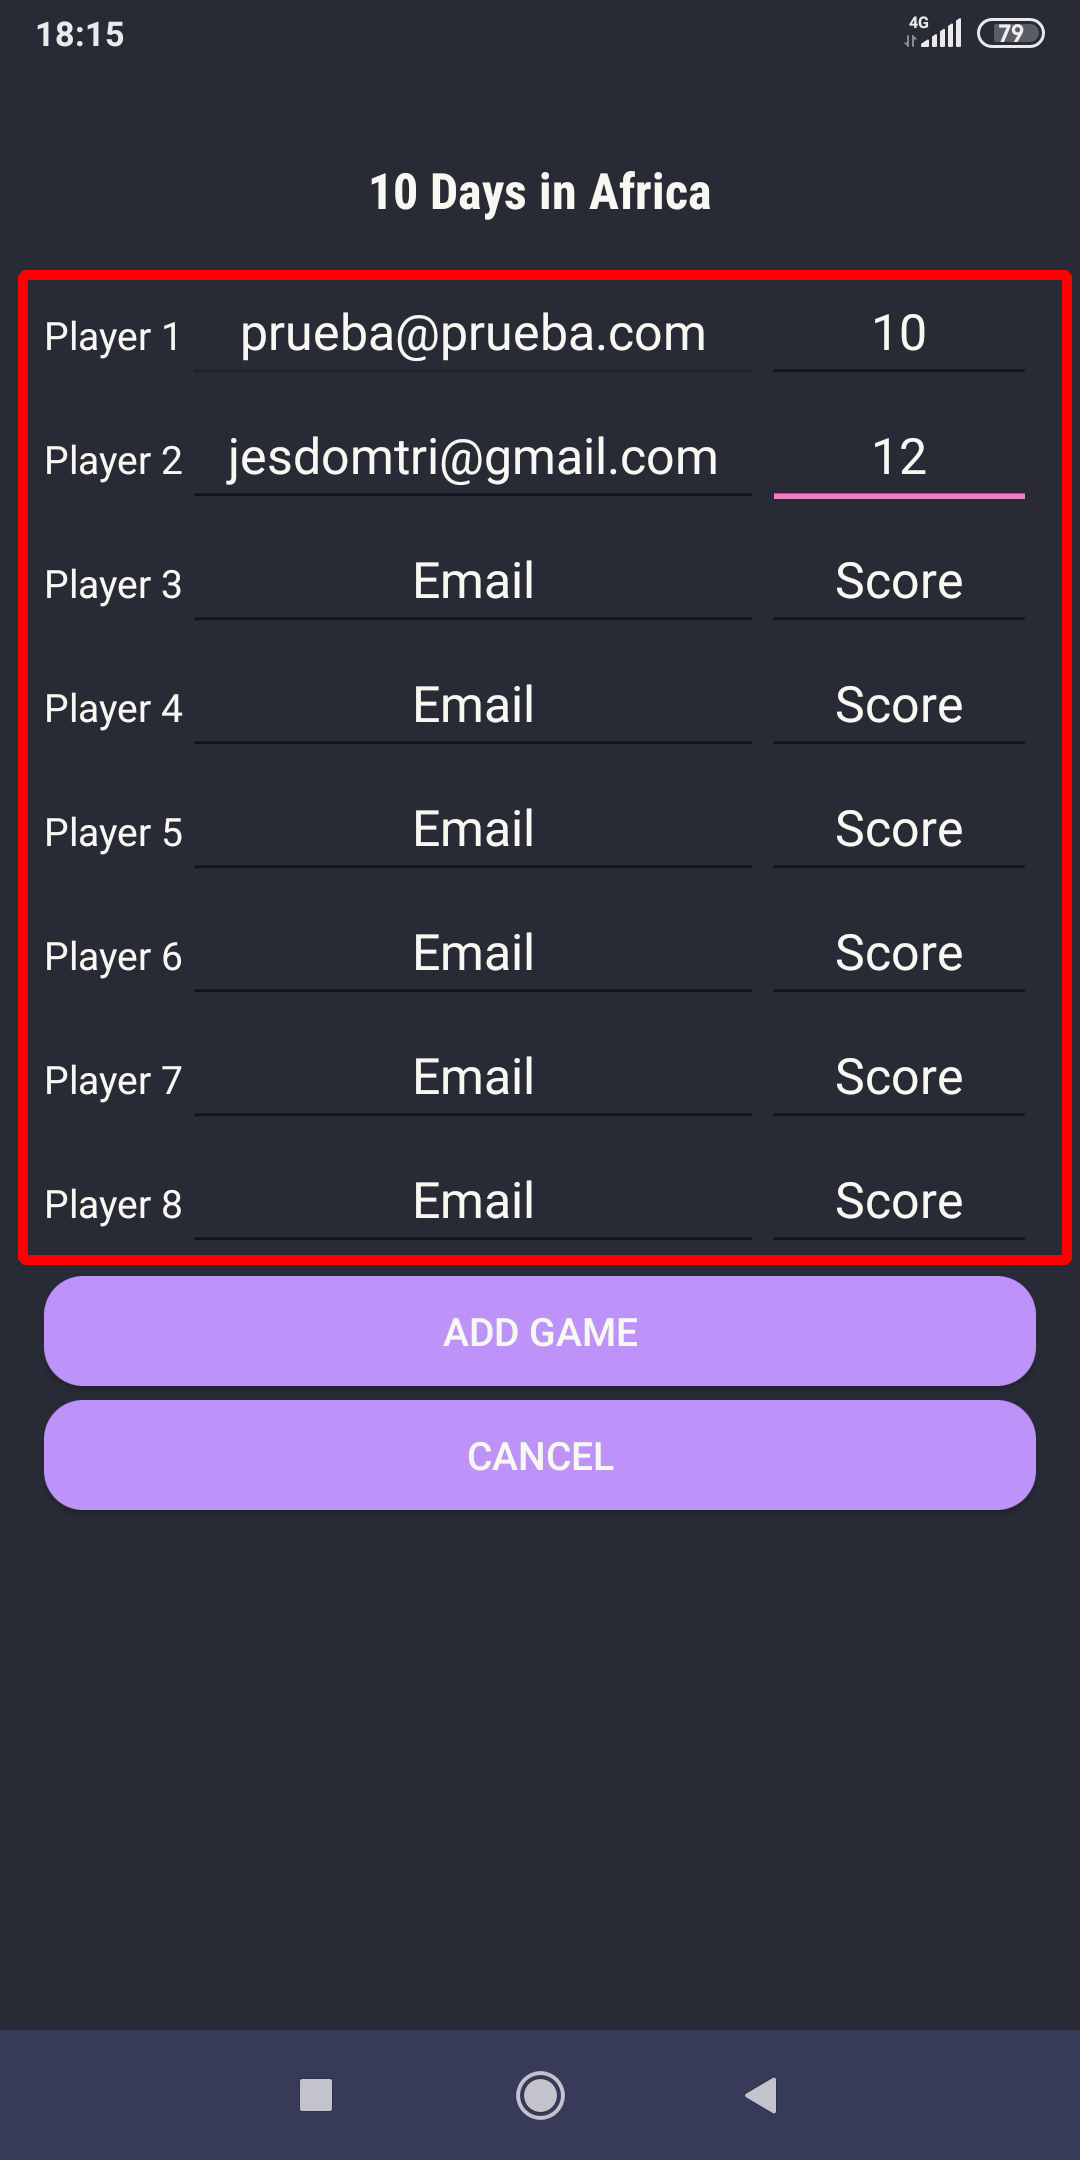
\includegraphics[width=0.3\linewidth]{fig/Uso/16.png}
    \caption{Añadir partida 1}
    \label{fig:uso16}
\end{figure}

\begin{figure}[H]
    \centering
    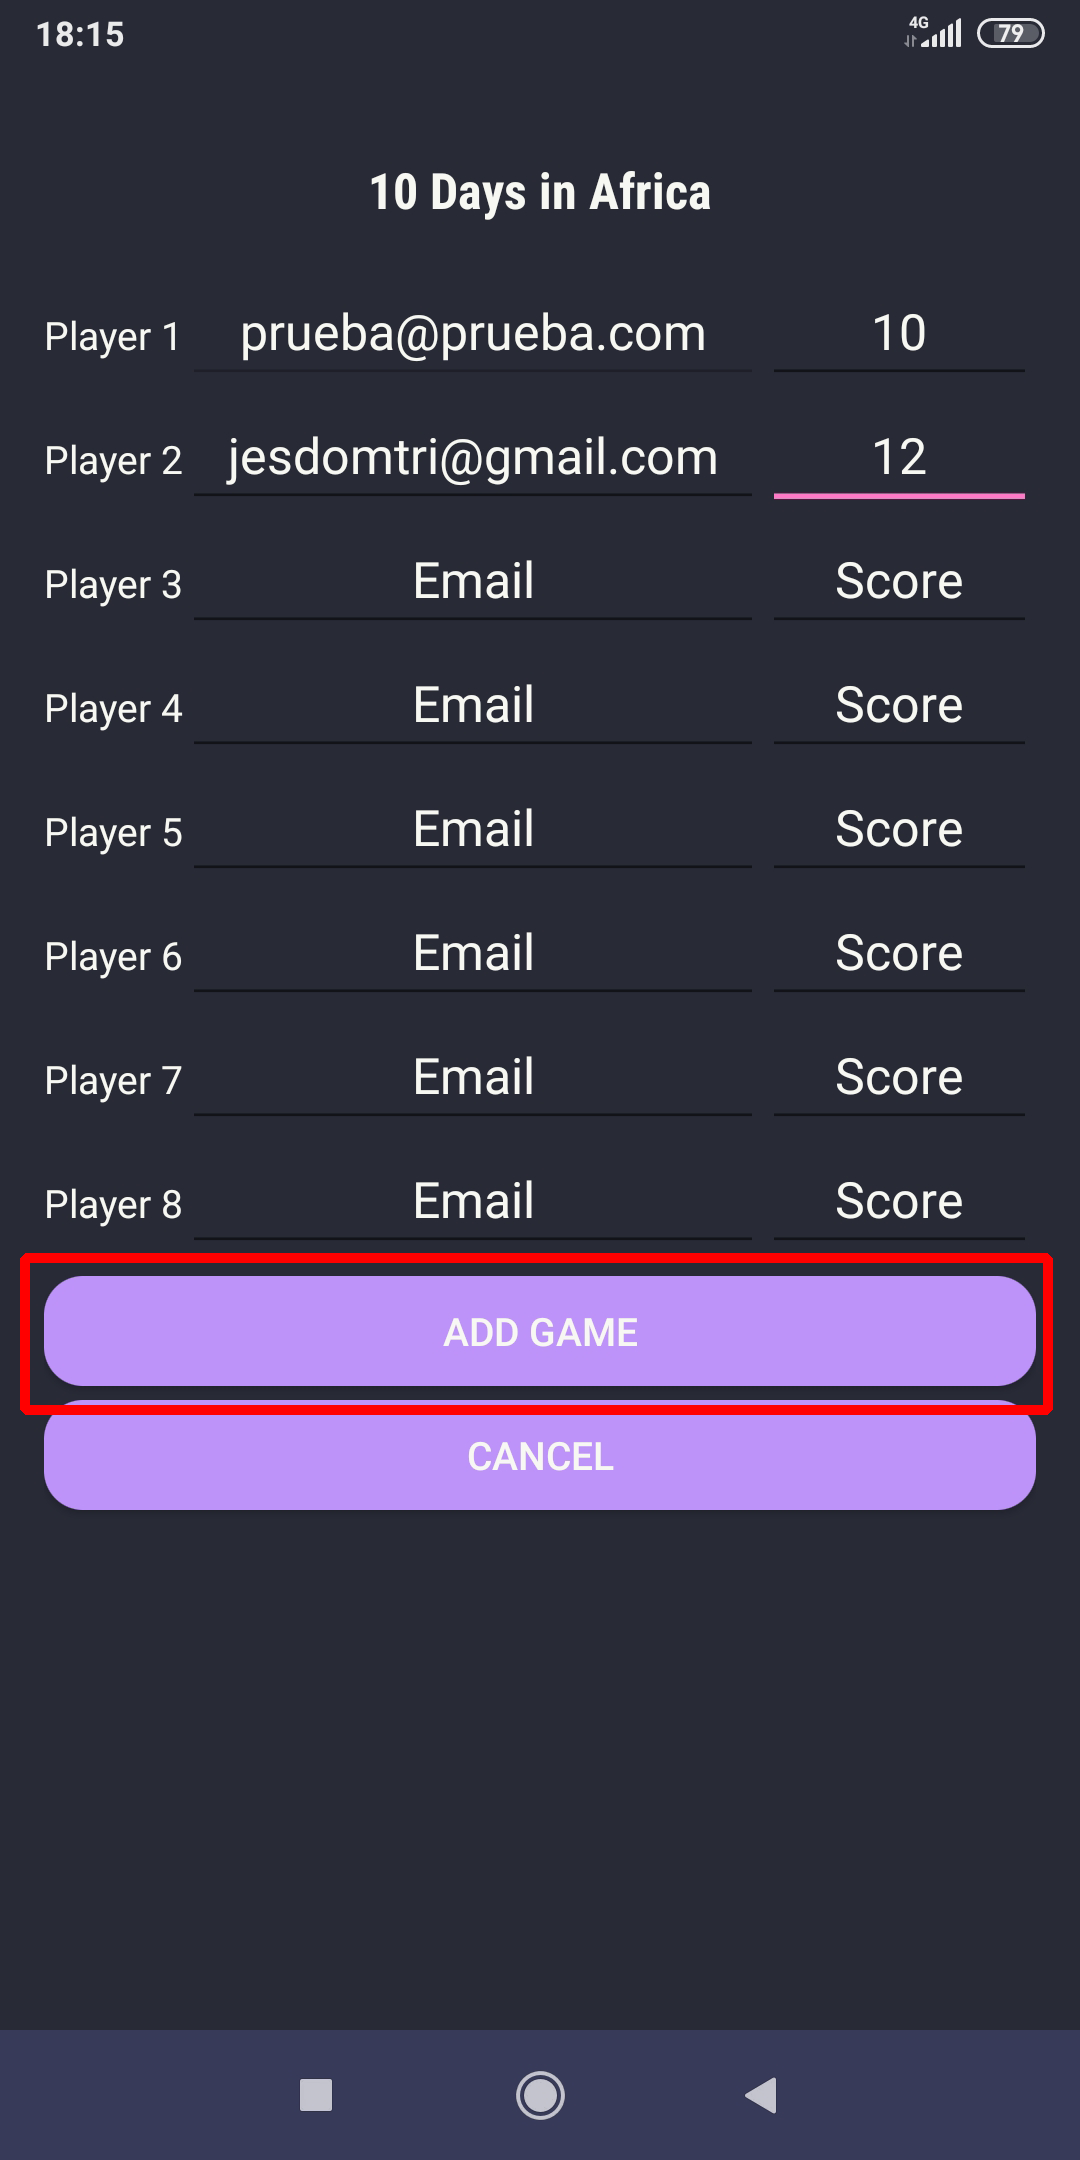
\includegraphics[width=0.3\linewidth]{fig/Uso/17.png}
    \caption{Añadir partida 2}
    \label{fig:uso17}
\end{figure}

Registrando dos partidas nos quedará algo como lo siguiente.

\begin{figure}[H]
    \centering
    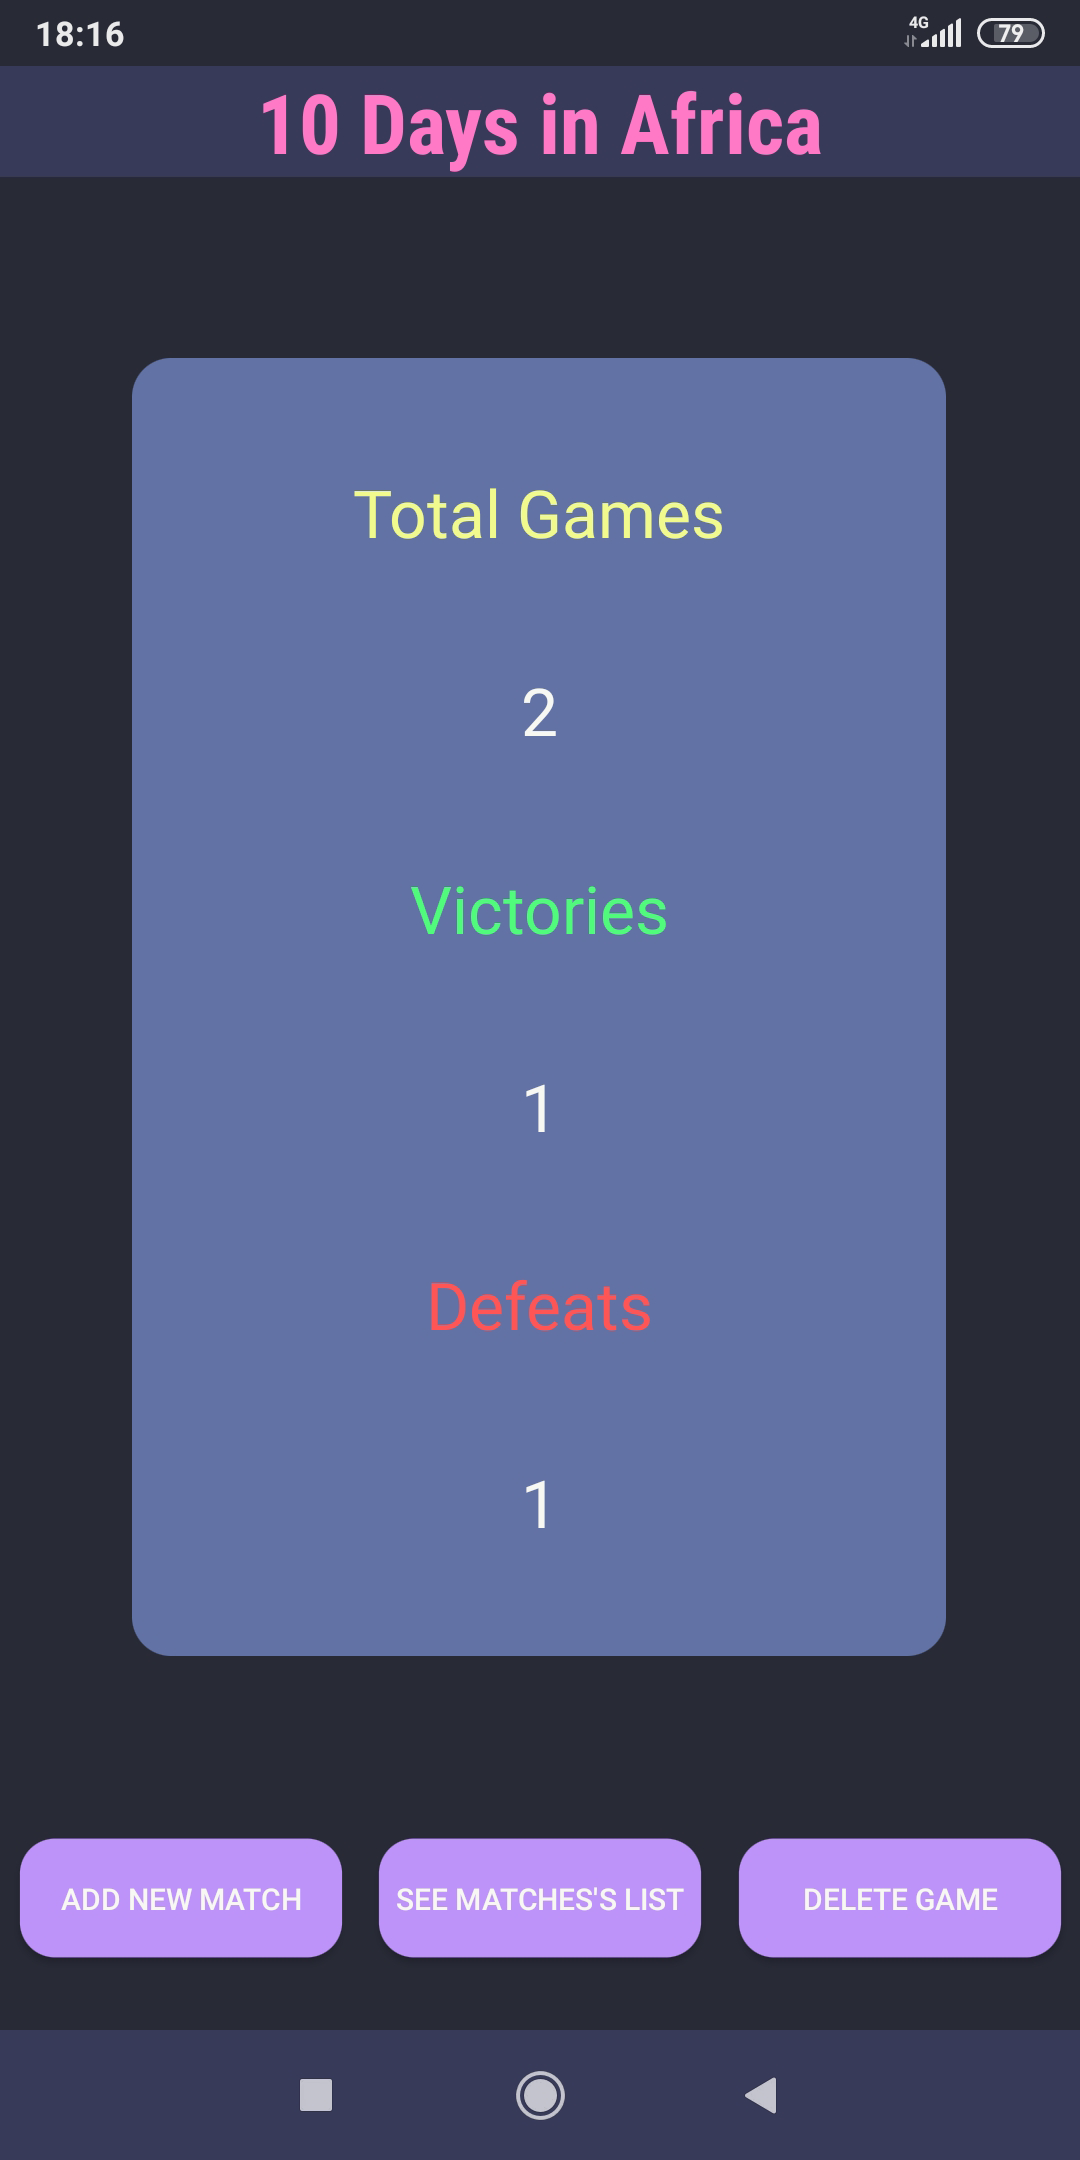
\includegraphics[width=0.3\linewidth]{fig/Uso/18.png}
    \caption{Partidas añadidas}
    \label{fig:uso18}
\end{figure}

Pulsando el botón para ver la lista de partidas de ese juego

\begin{figure}[H]
    \centering
    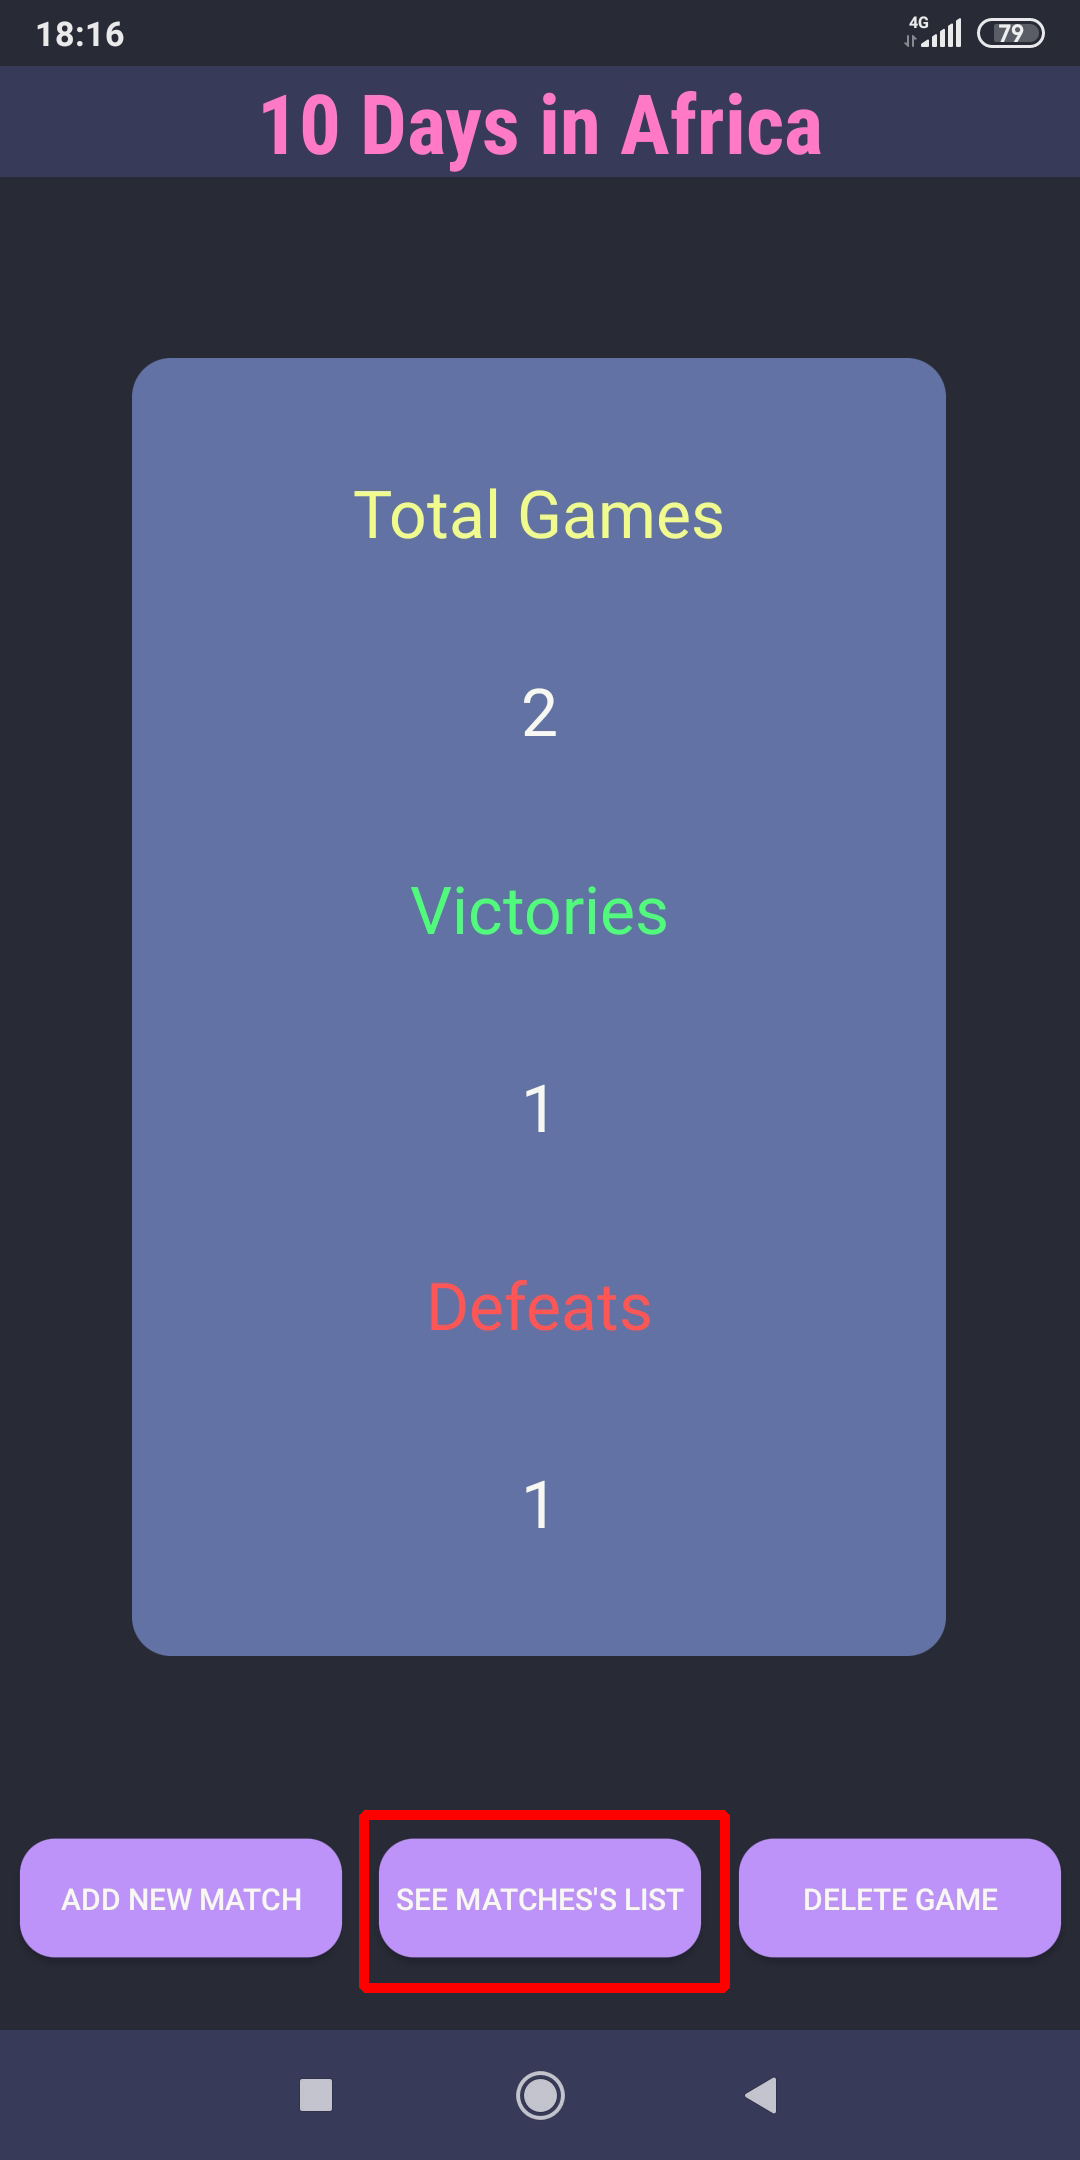
\includegraphics[width=0.3\linewidth]{fig/Uso/19.png}
    \caption{Botón de lista de partidas}
    \label{fig:uso19}
\end{figure}

nos mostrará la siguiente ventana con una lista de partidas reflejando nuestra puntuación, posición y una corona que solamente se mostrará en las partidas que hayamos acabado en primera posición.

\begin{figure}[H]
    \centering
    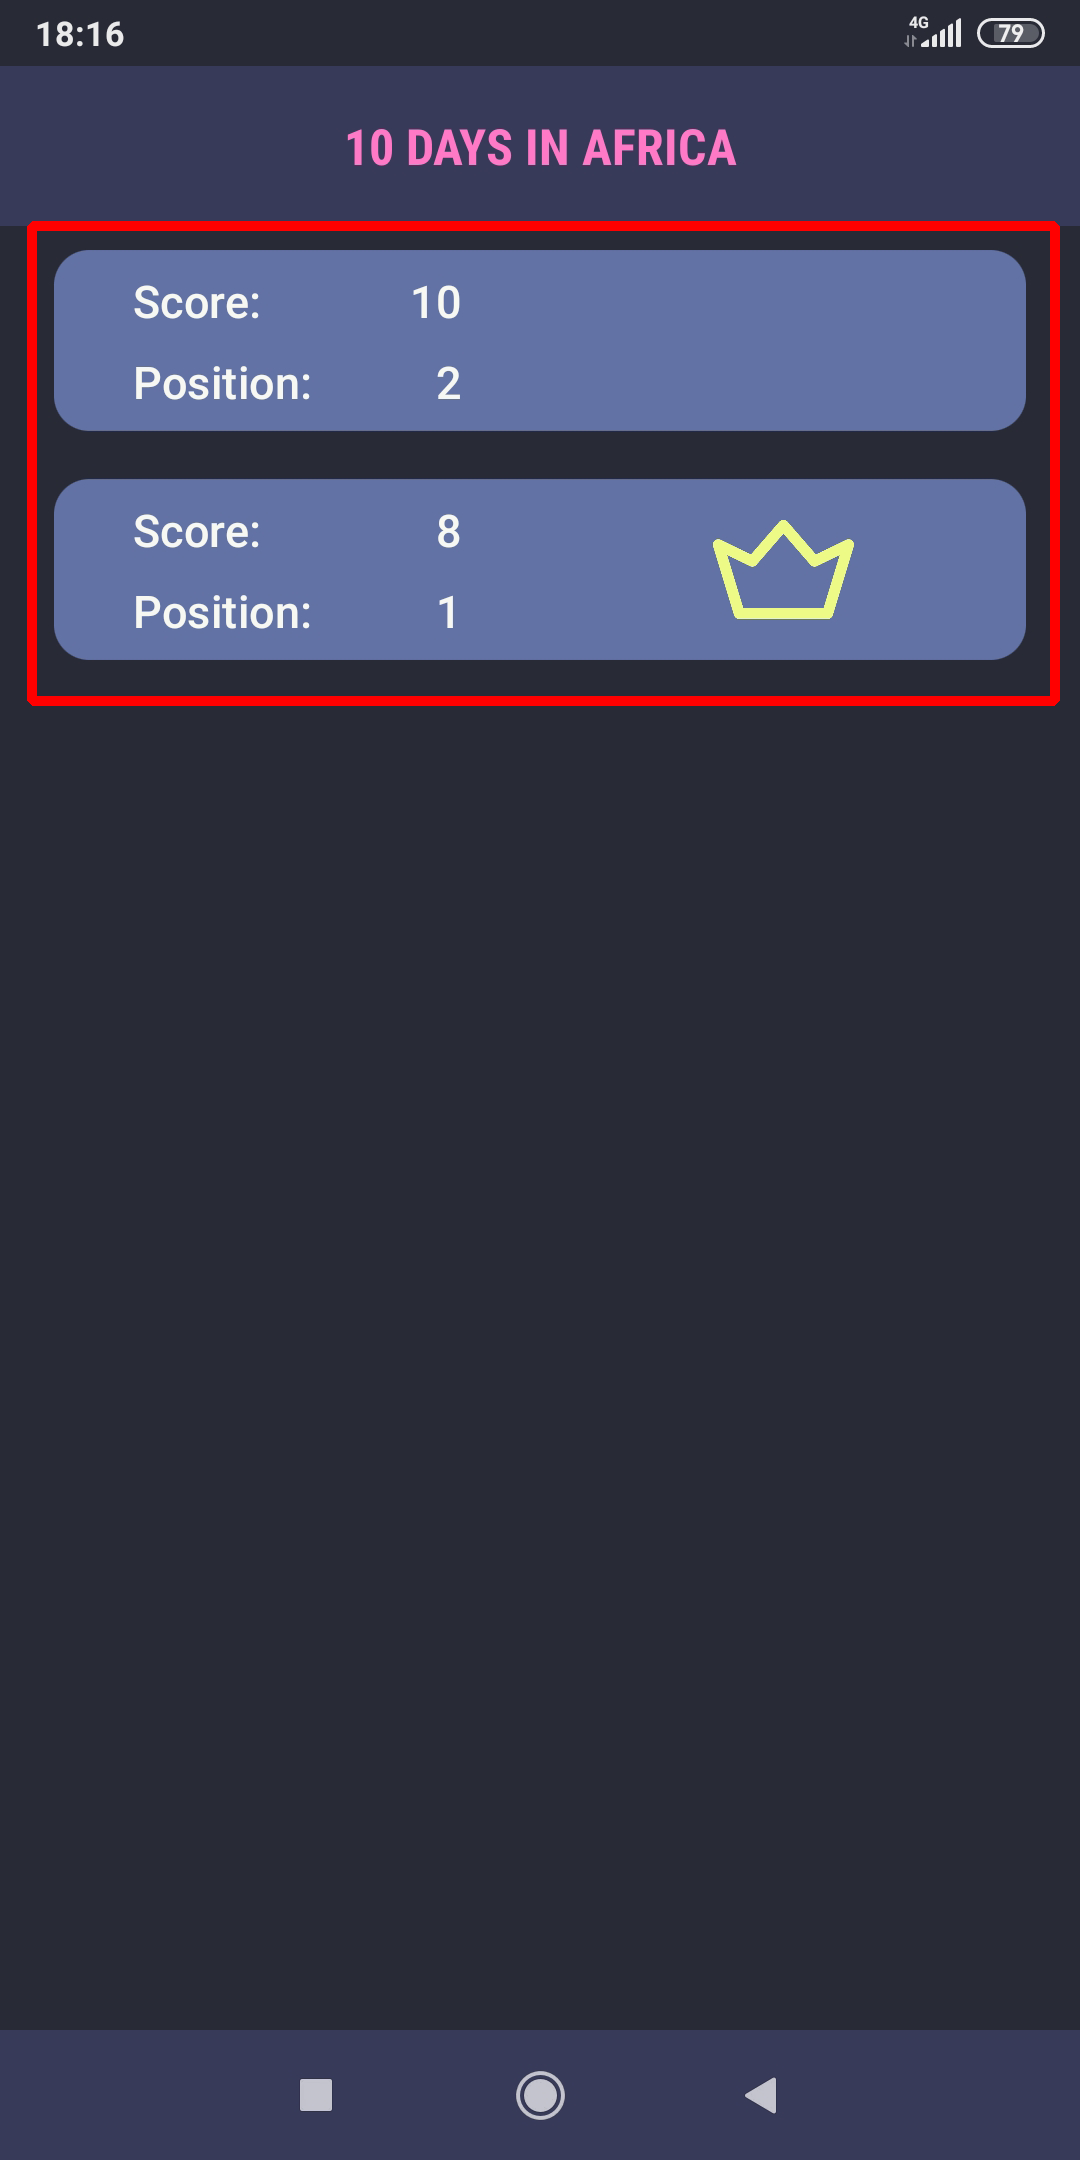
\includegraphics[width=0.3\linewidth]{fig/Uso/20.png}
    \caption{Lista de partidas}
    \label{fig:uso20}
\end{figure}

Por último, pulsando el tercer botón, borraremos este juego de la lista de juegos favoritos, cuya acción también nos será notificada como cuando añadimos un juego, mediante un mensaje al usuario en pantalla.

\begin{figure}[H]
    \centering
    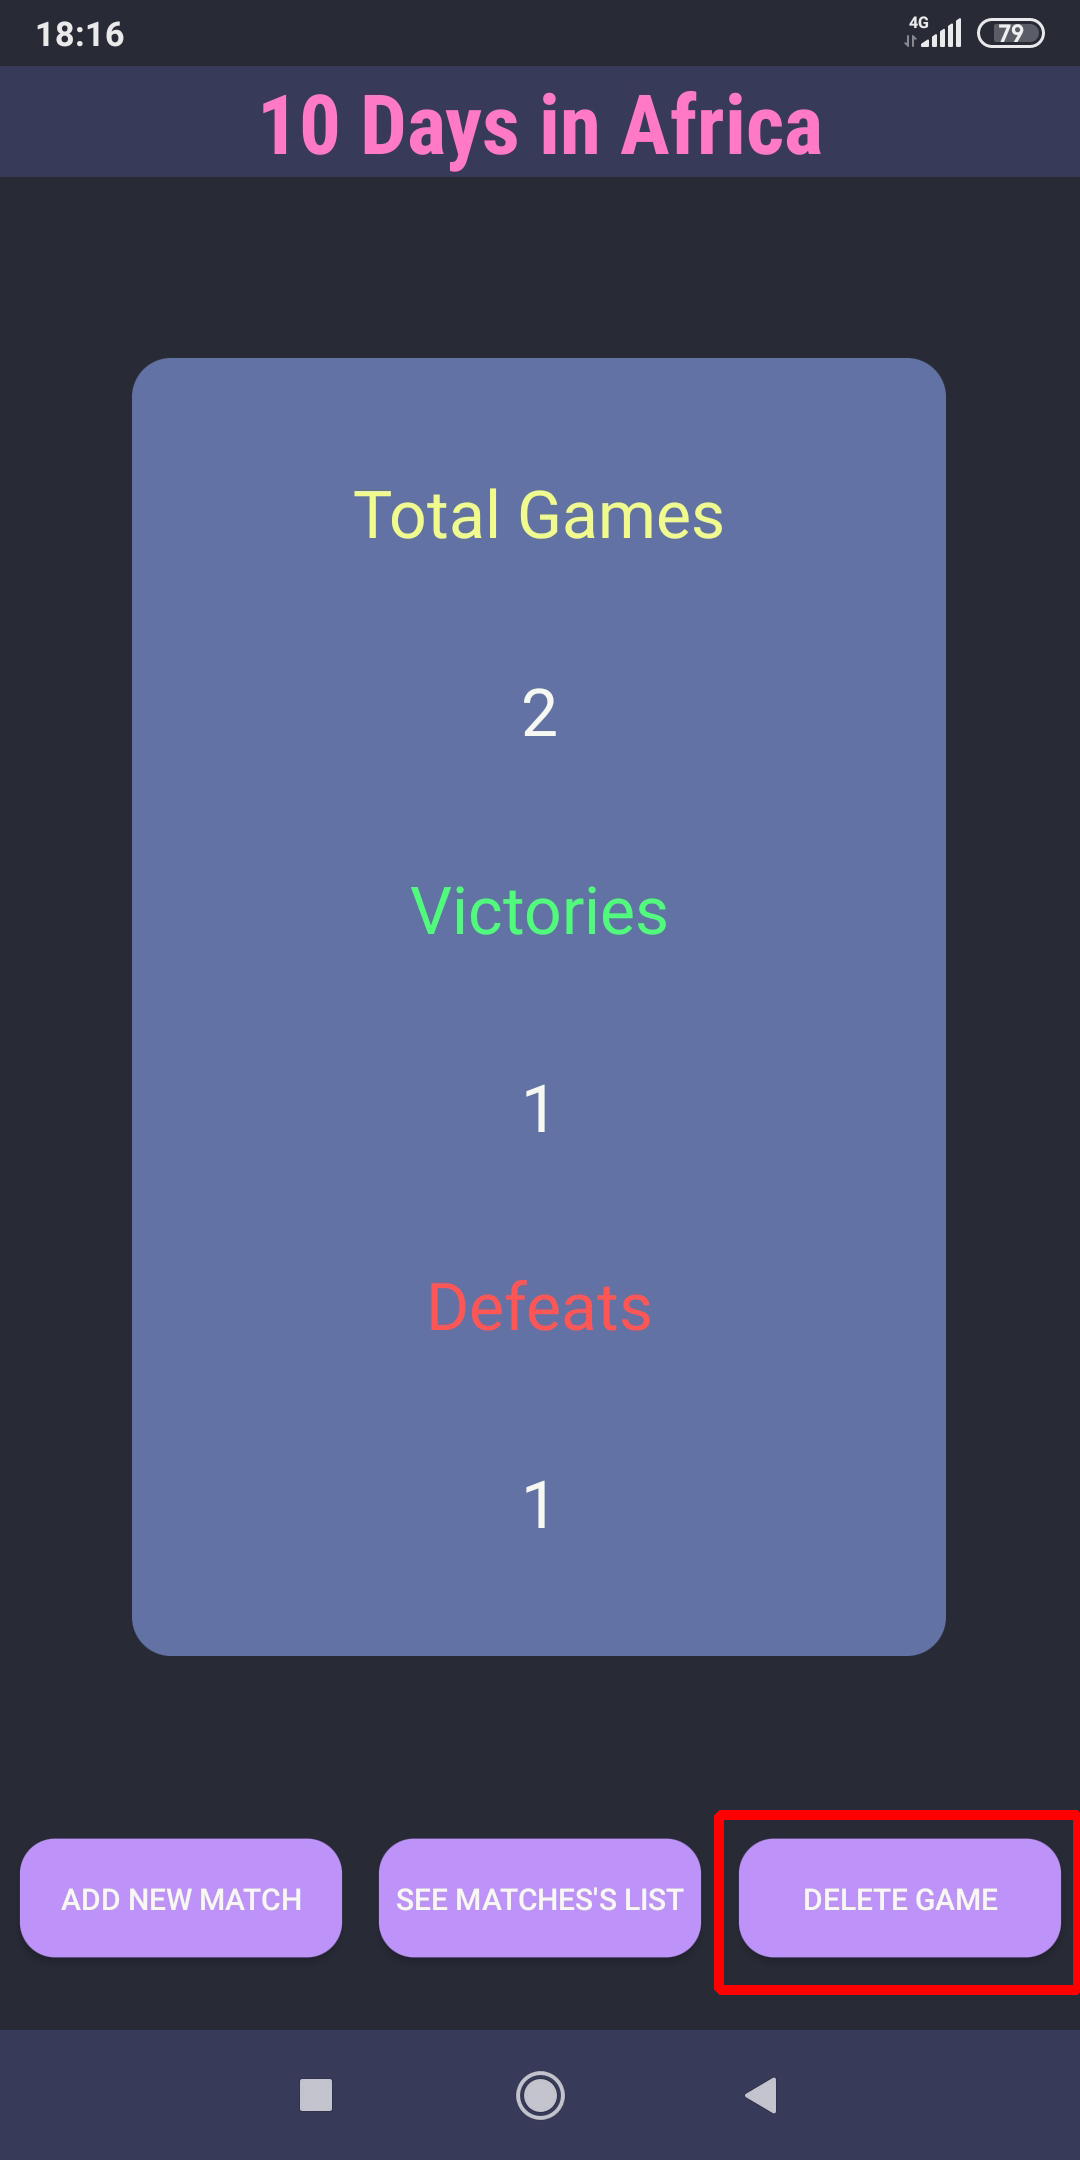
\includegraphics[width=0.3\linewidth]{fig/Uso/21.png}
    \caption{Borrar juego favorito 1}
    \label{fig:uso21}
\end{figure}

\begin{figure}[H]
    \centering
    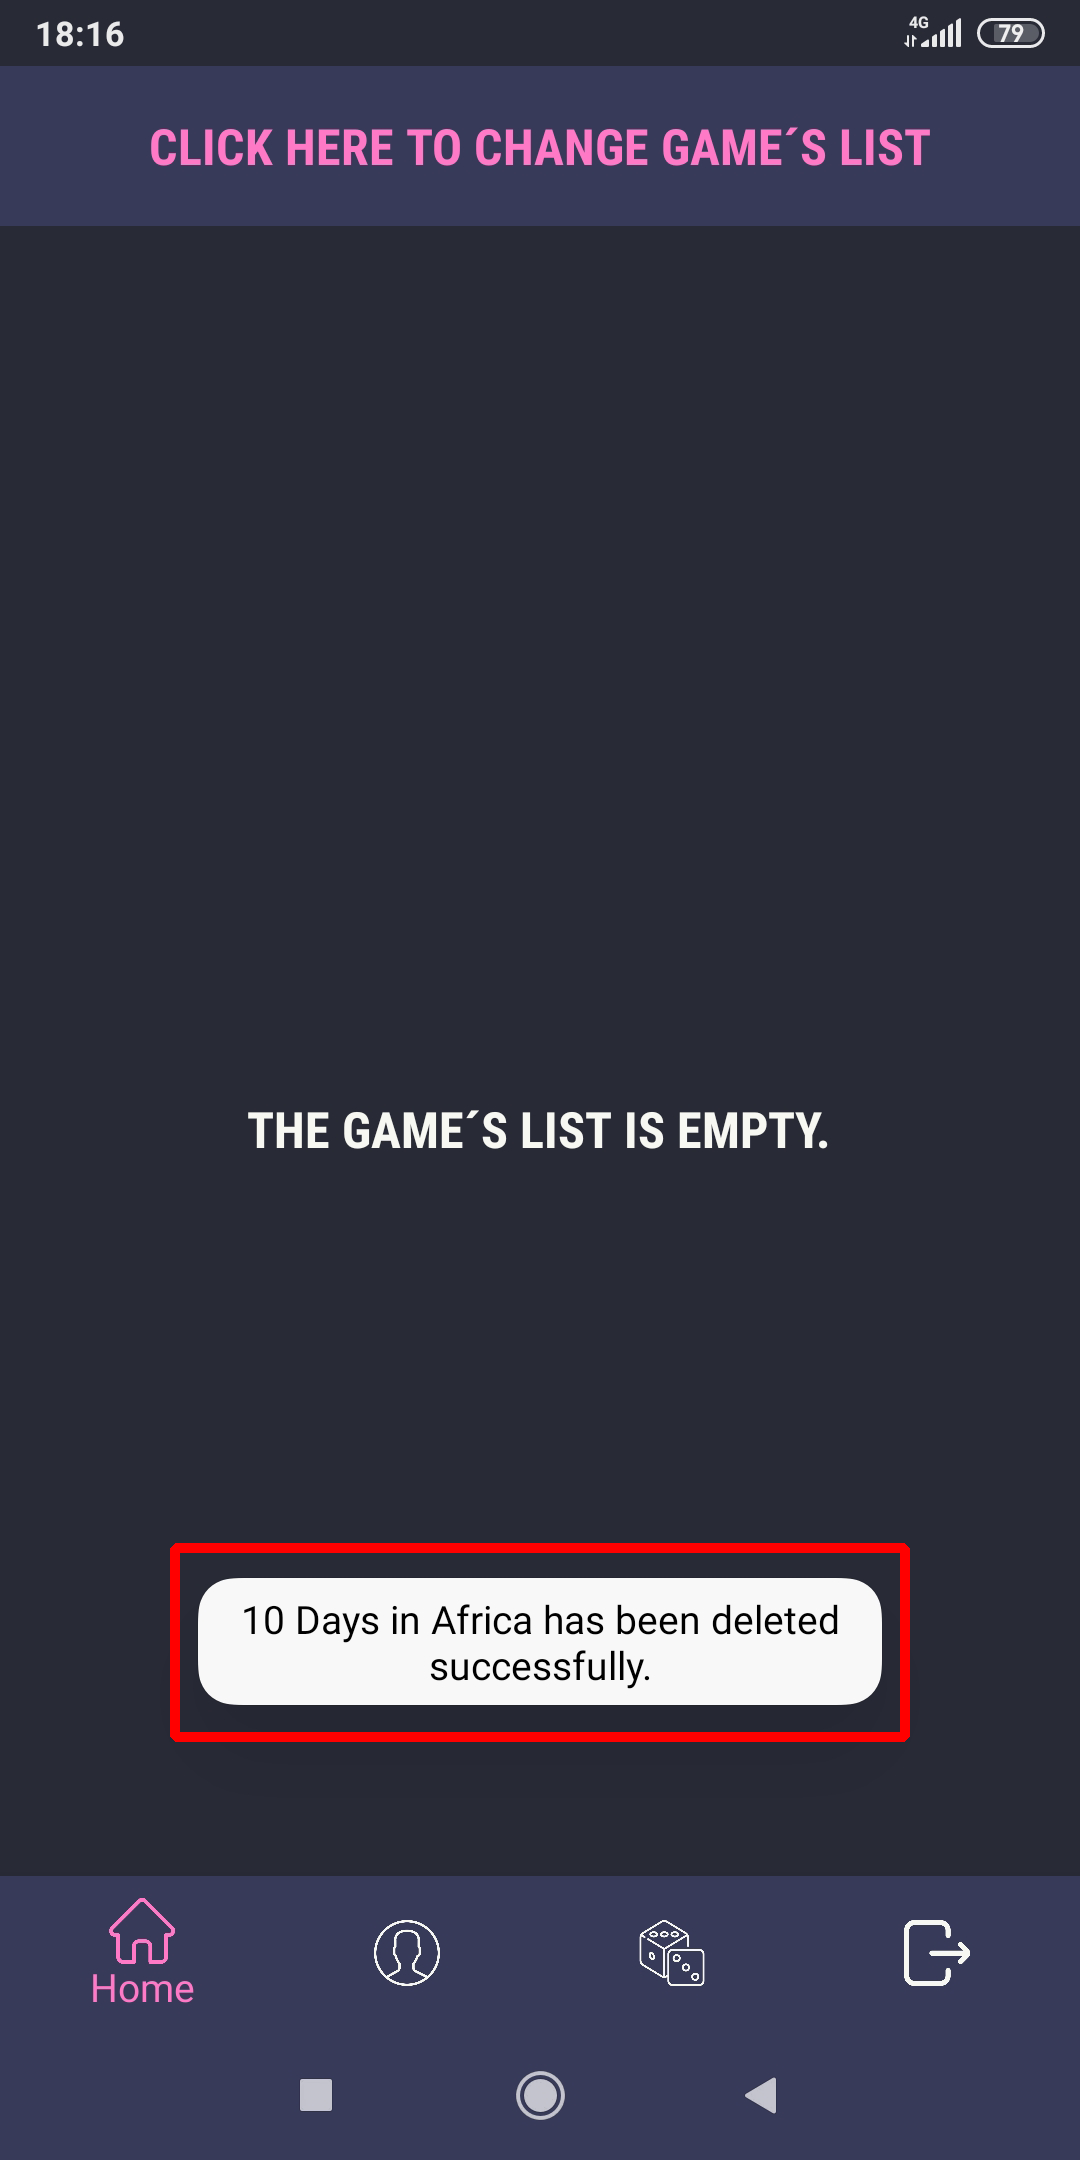
\includegraphics[width=0.3\linewidth]{fig/Uso/22.png}
    \caption{Borrar juego favorito 2}
    \label{fig:uso22}
\end{figure}

Desde la segunda ventana que nos abrirá la barra de navegación podremos ver nuestros datos de usuario. En específico, nuestro correo electrónico, contraseña modificada con asteriscos, un botón para restablecer esta última, nuestro identificador de usuario y la fecha en la que nos registramos.

\begin{figure}[H]
    \centering
    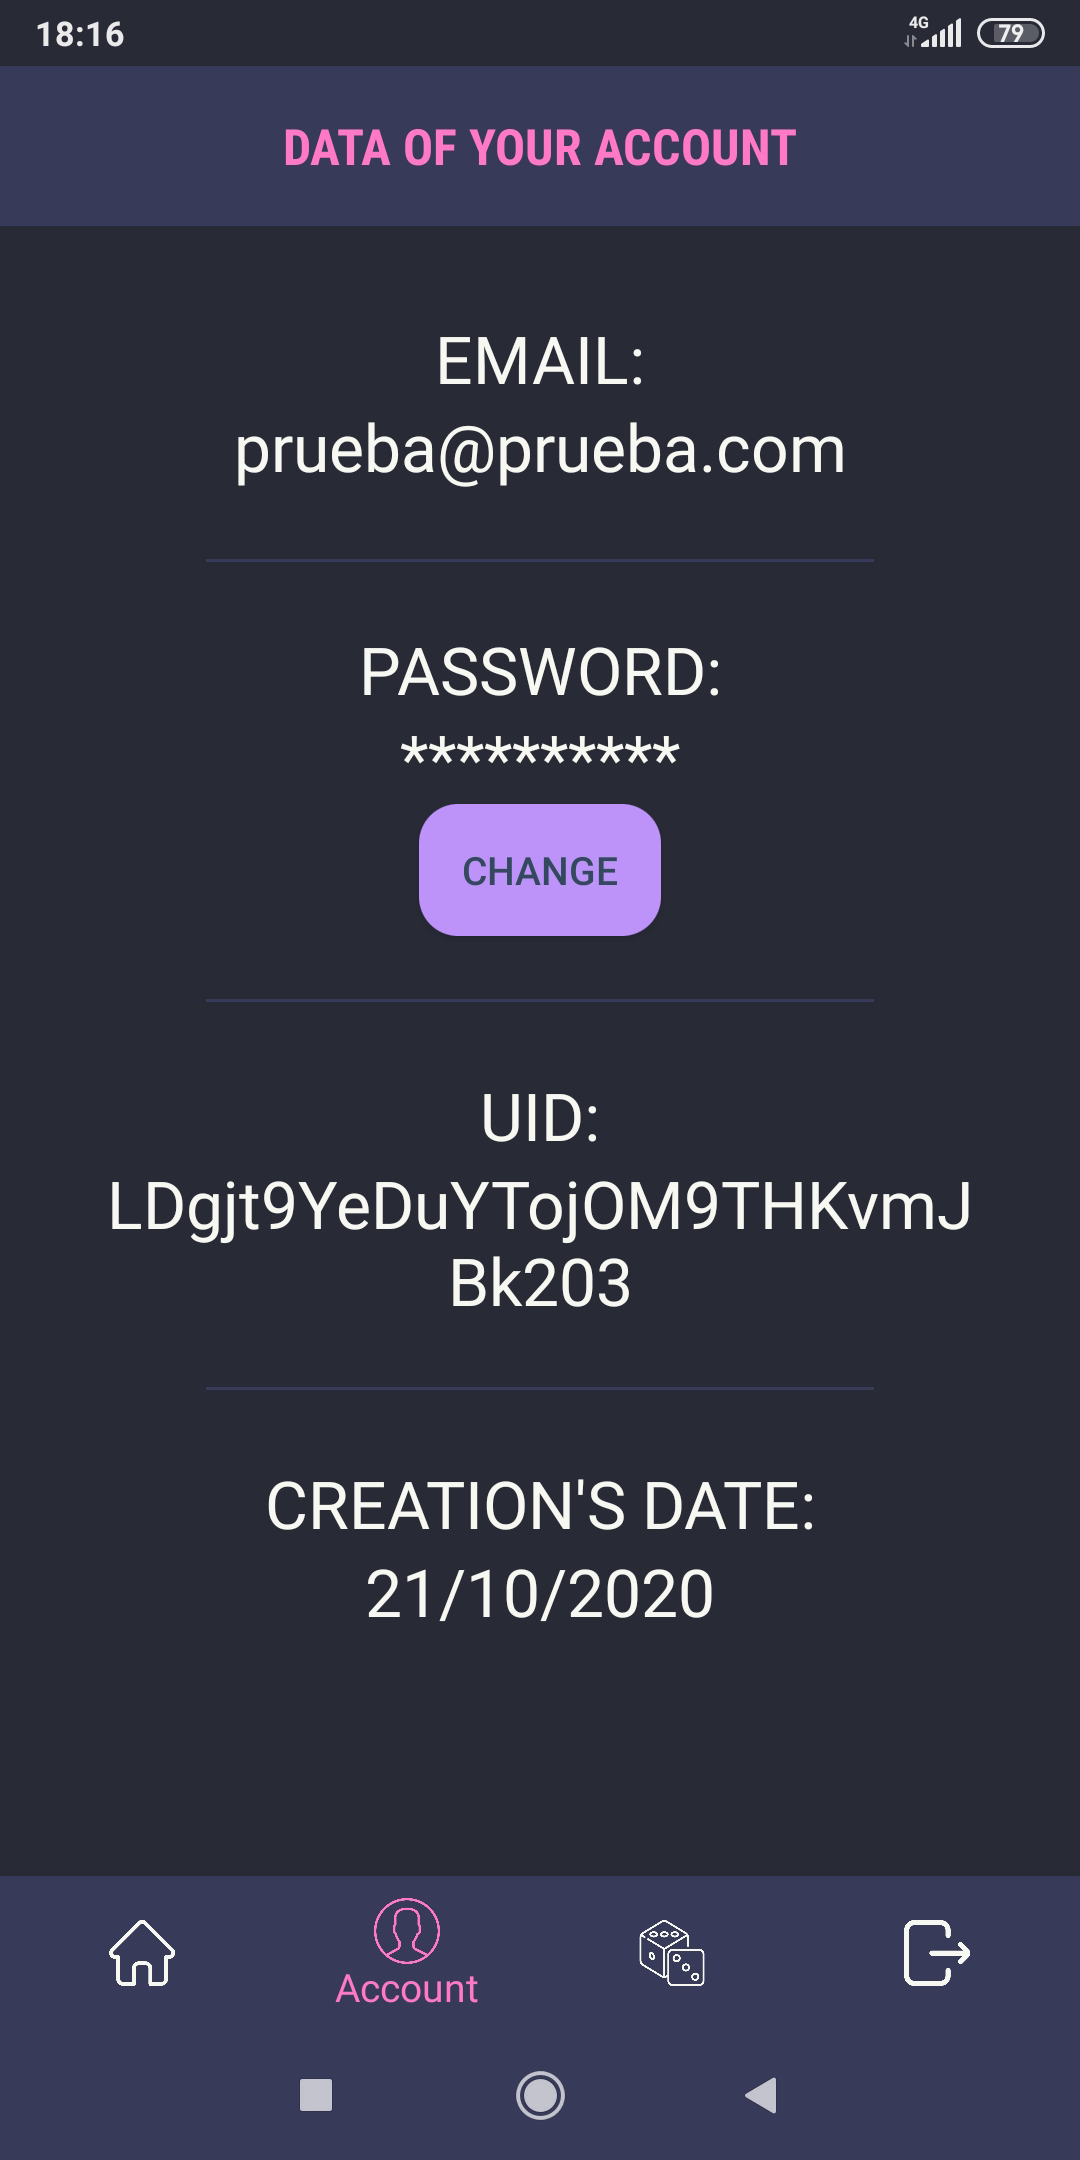
\includegraphics[width=0.3\linewidth]{fig/Uso/23.png}
    \caption{Datos de usuario 1}
    \label{fig:uso23}
\end{figure}

\begin{figure}[H]
    \centering
    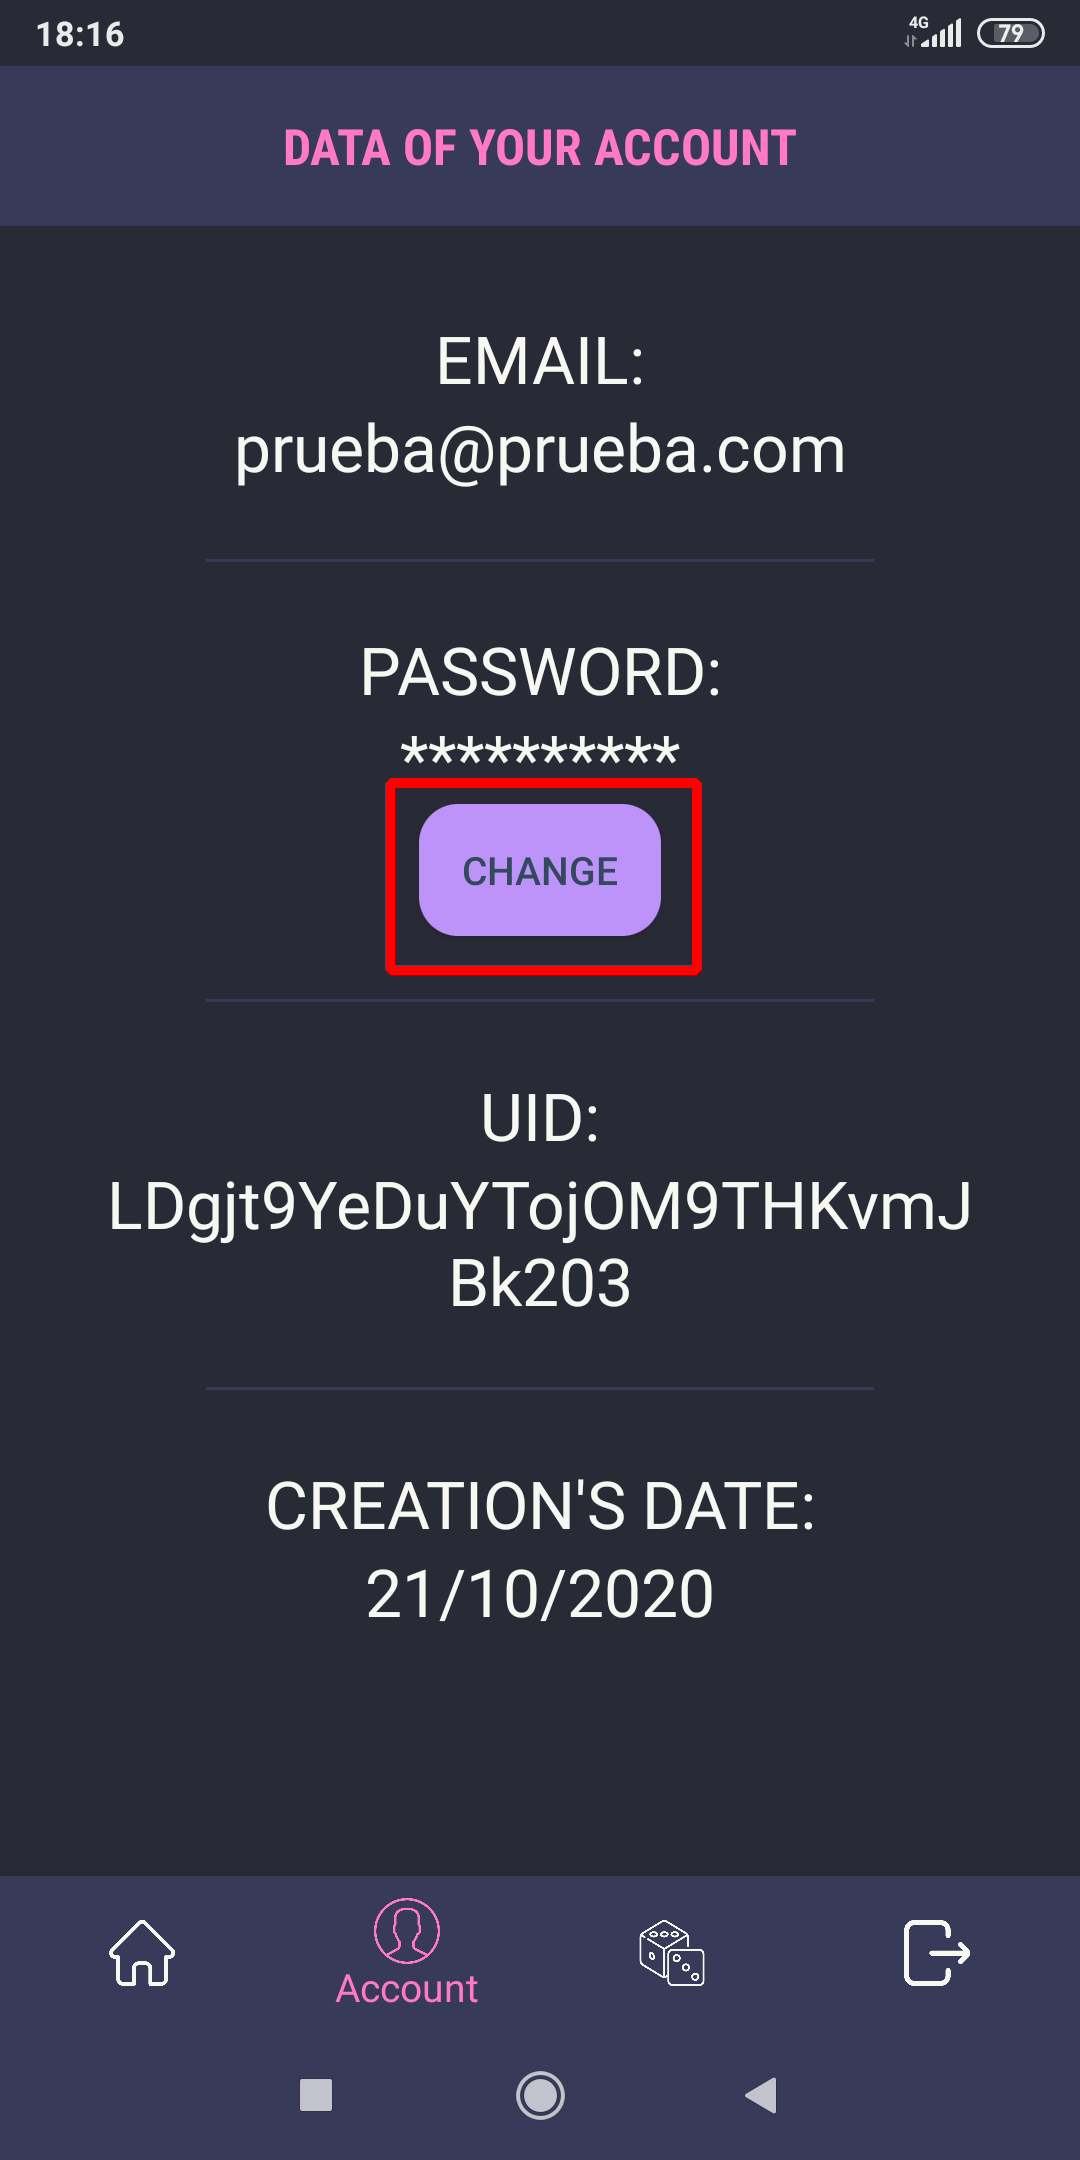
\includegraphics[width=0.3\linewidth]{fig/Uso/24.png}
    \caption{Datos de usuario 2}
    \label{fig:uso24}
\end{figure}

\begin{figure}[H]
    \centering
    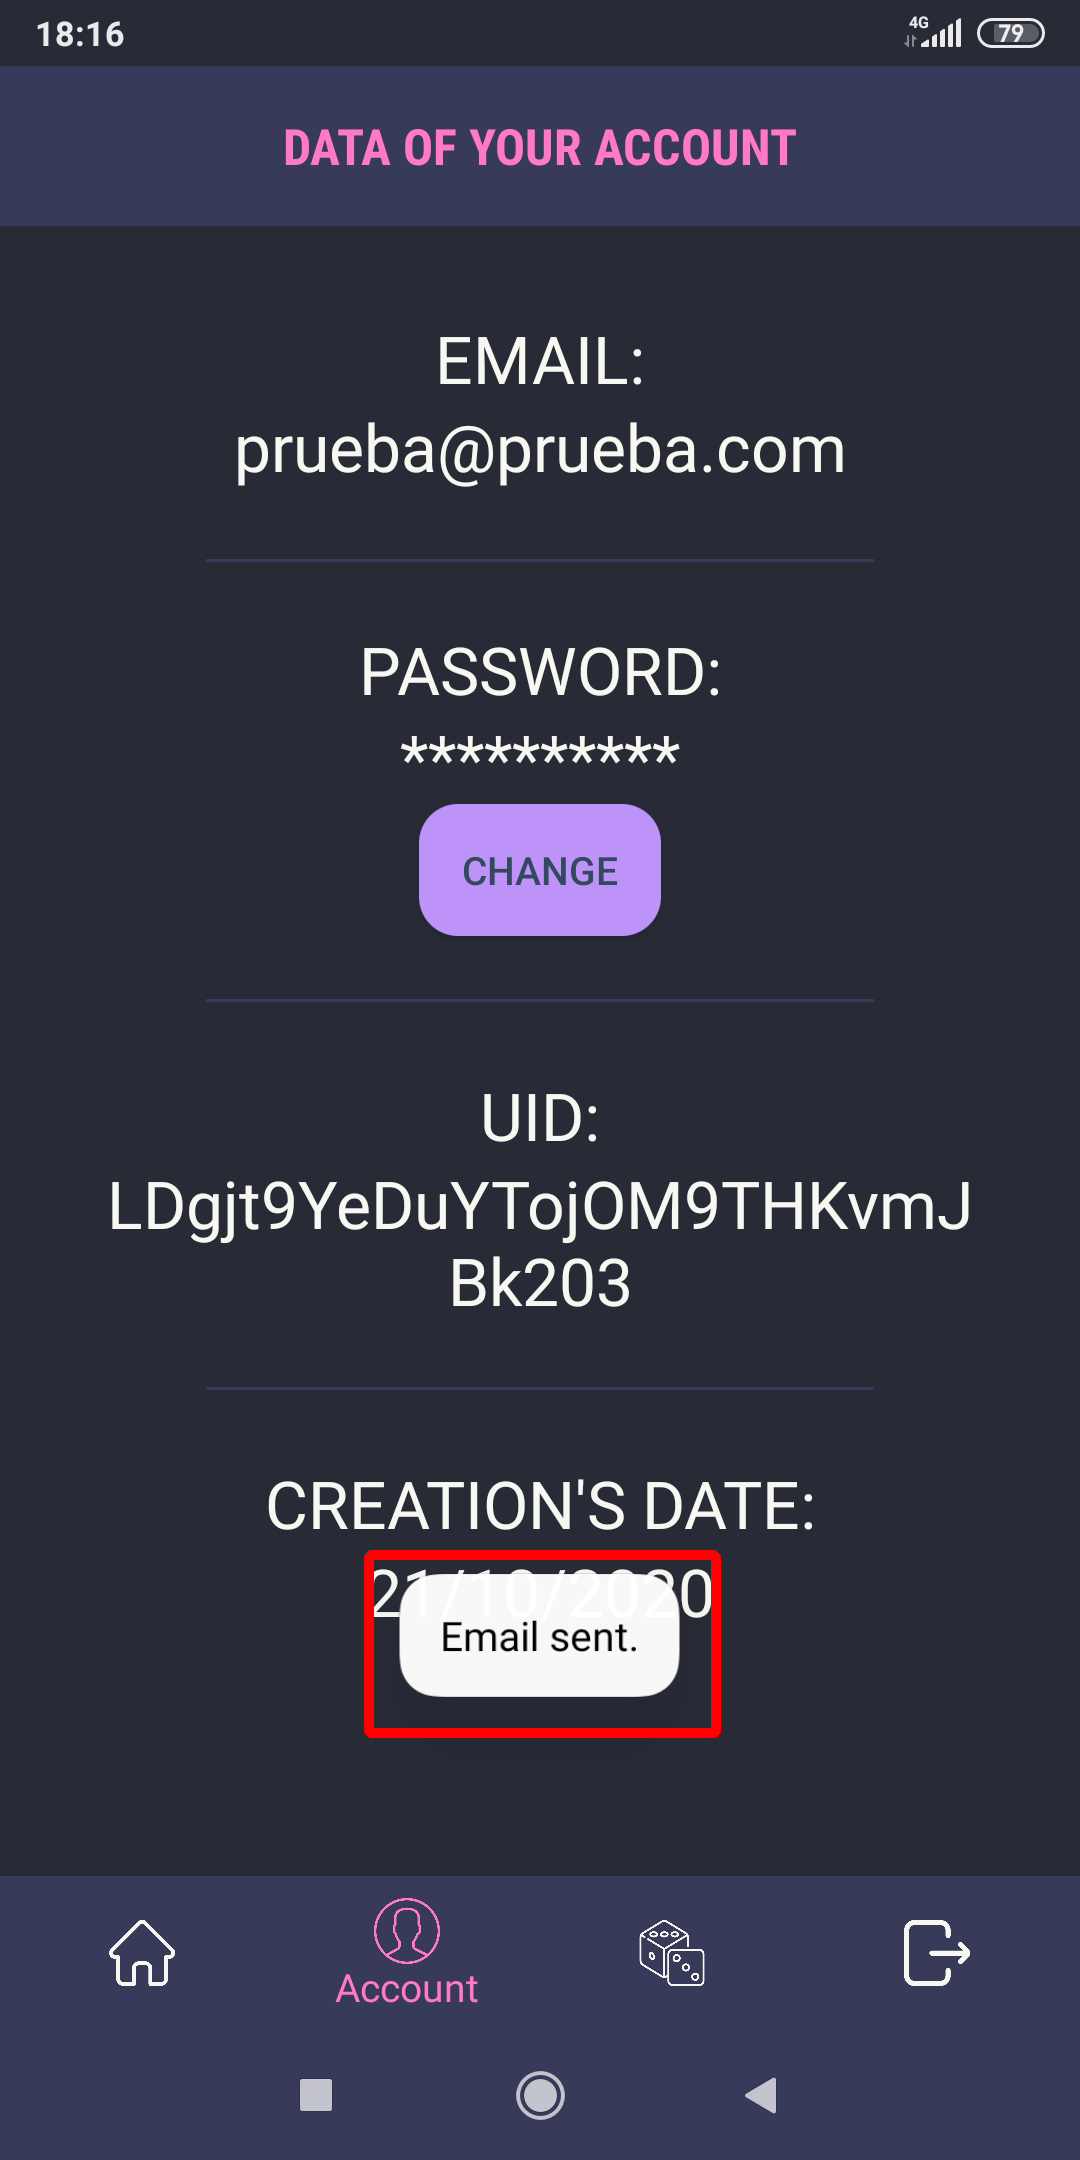
\includegraphics[width=0.3\linewidth]{fig/Uso/25.png}
    \caption{Datos de usuario 3}
    \label{fig:uso25}
\end{figure}

Por último, tenemos la última ventana de la barra de navegación en la que estarán las cuatro utilidades que se han creado para facilitar el transcurso de las partidas de juegos de mesa.

\begin{figure}[H]
    \centering
    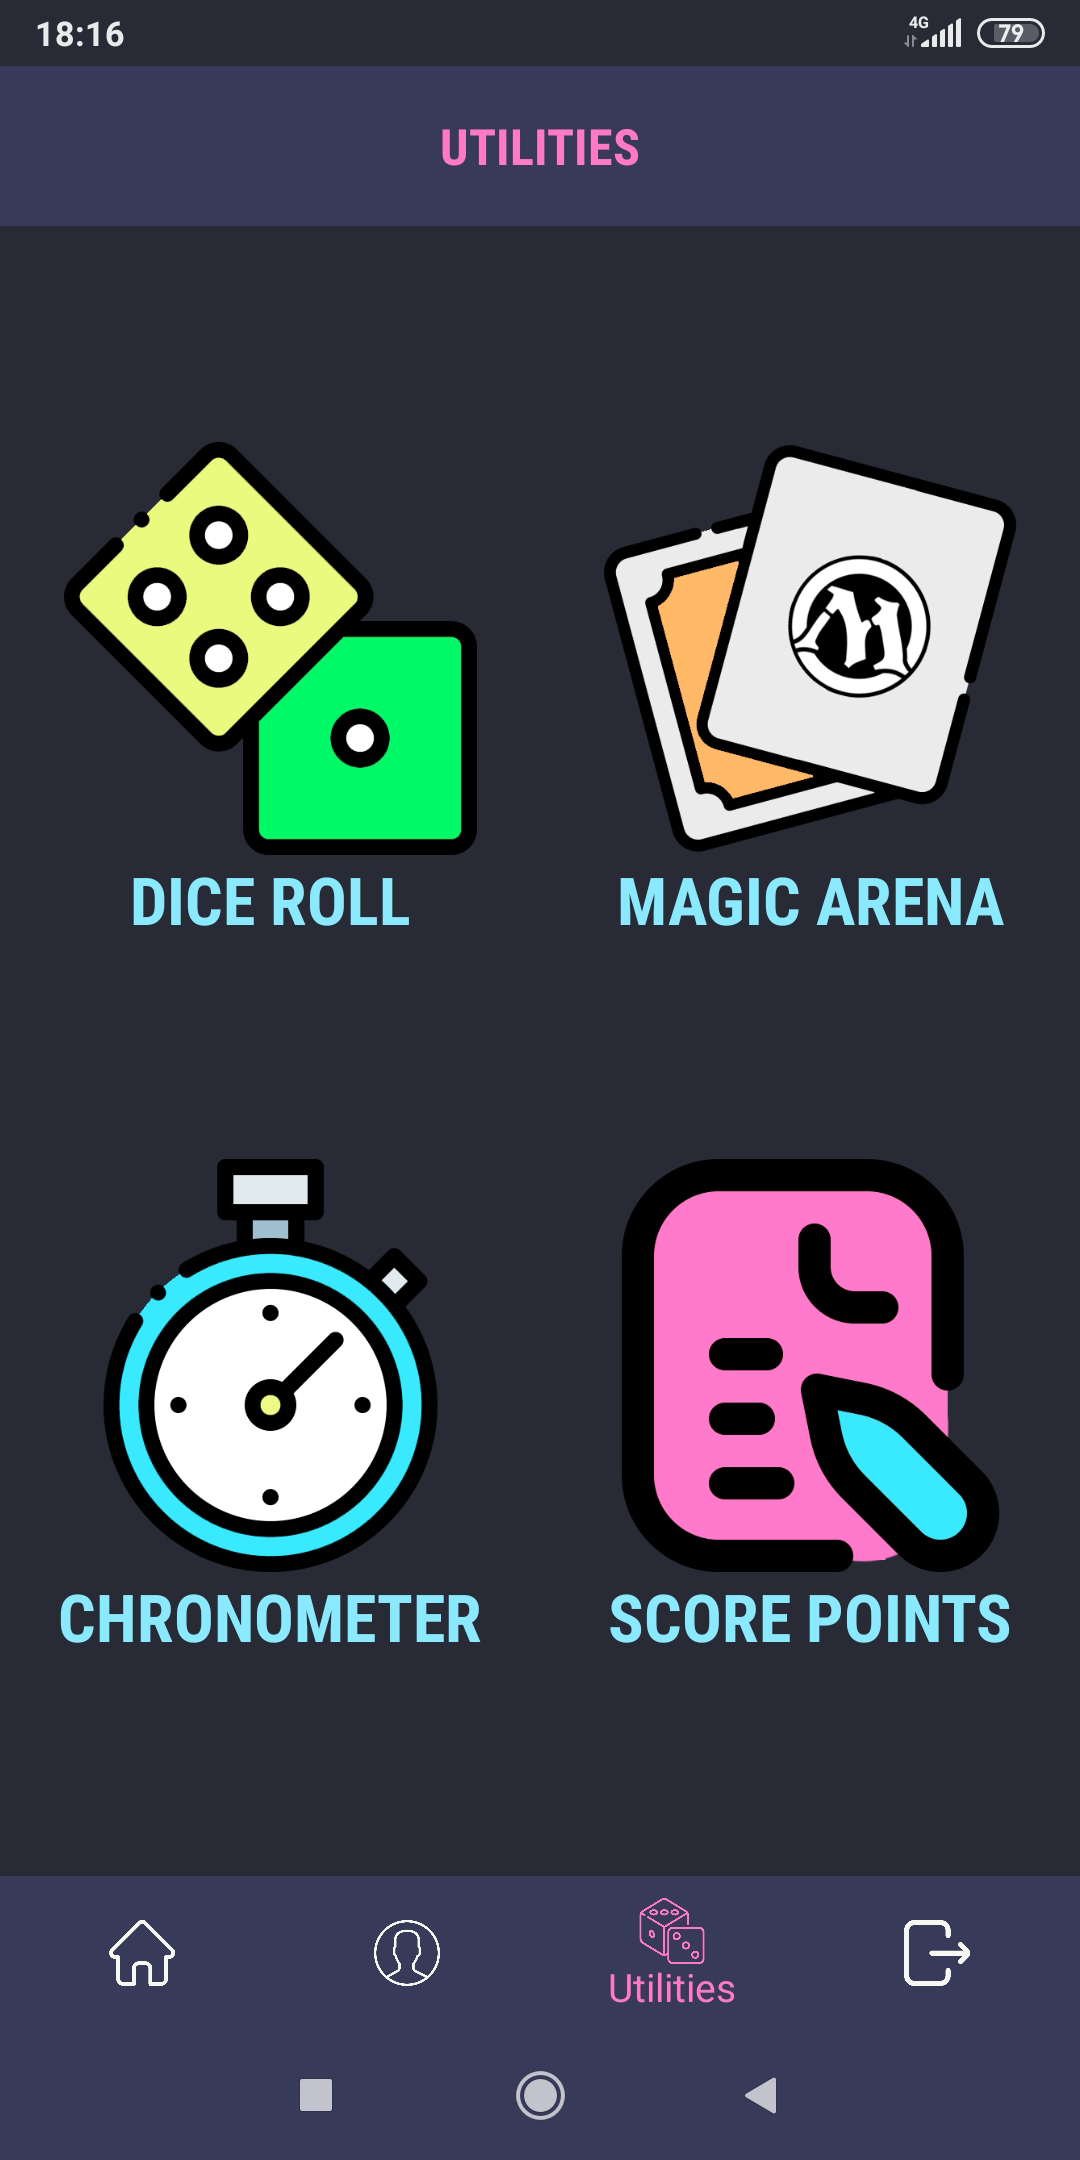
\includegraphics[width=0.3\linewidth]{fig/Uso/26.png}
    \caption{Ventana de utilidades}
    \label{fig:uso26}
\end{figure}

Dichas utilidades serán accesibles mediante 4 imágenes.

\begin{figure}[H]
    \centering
    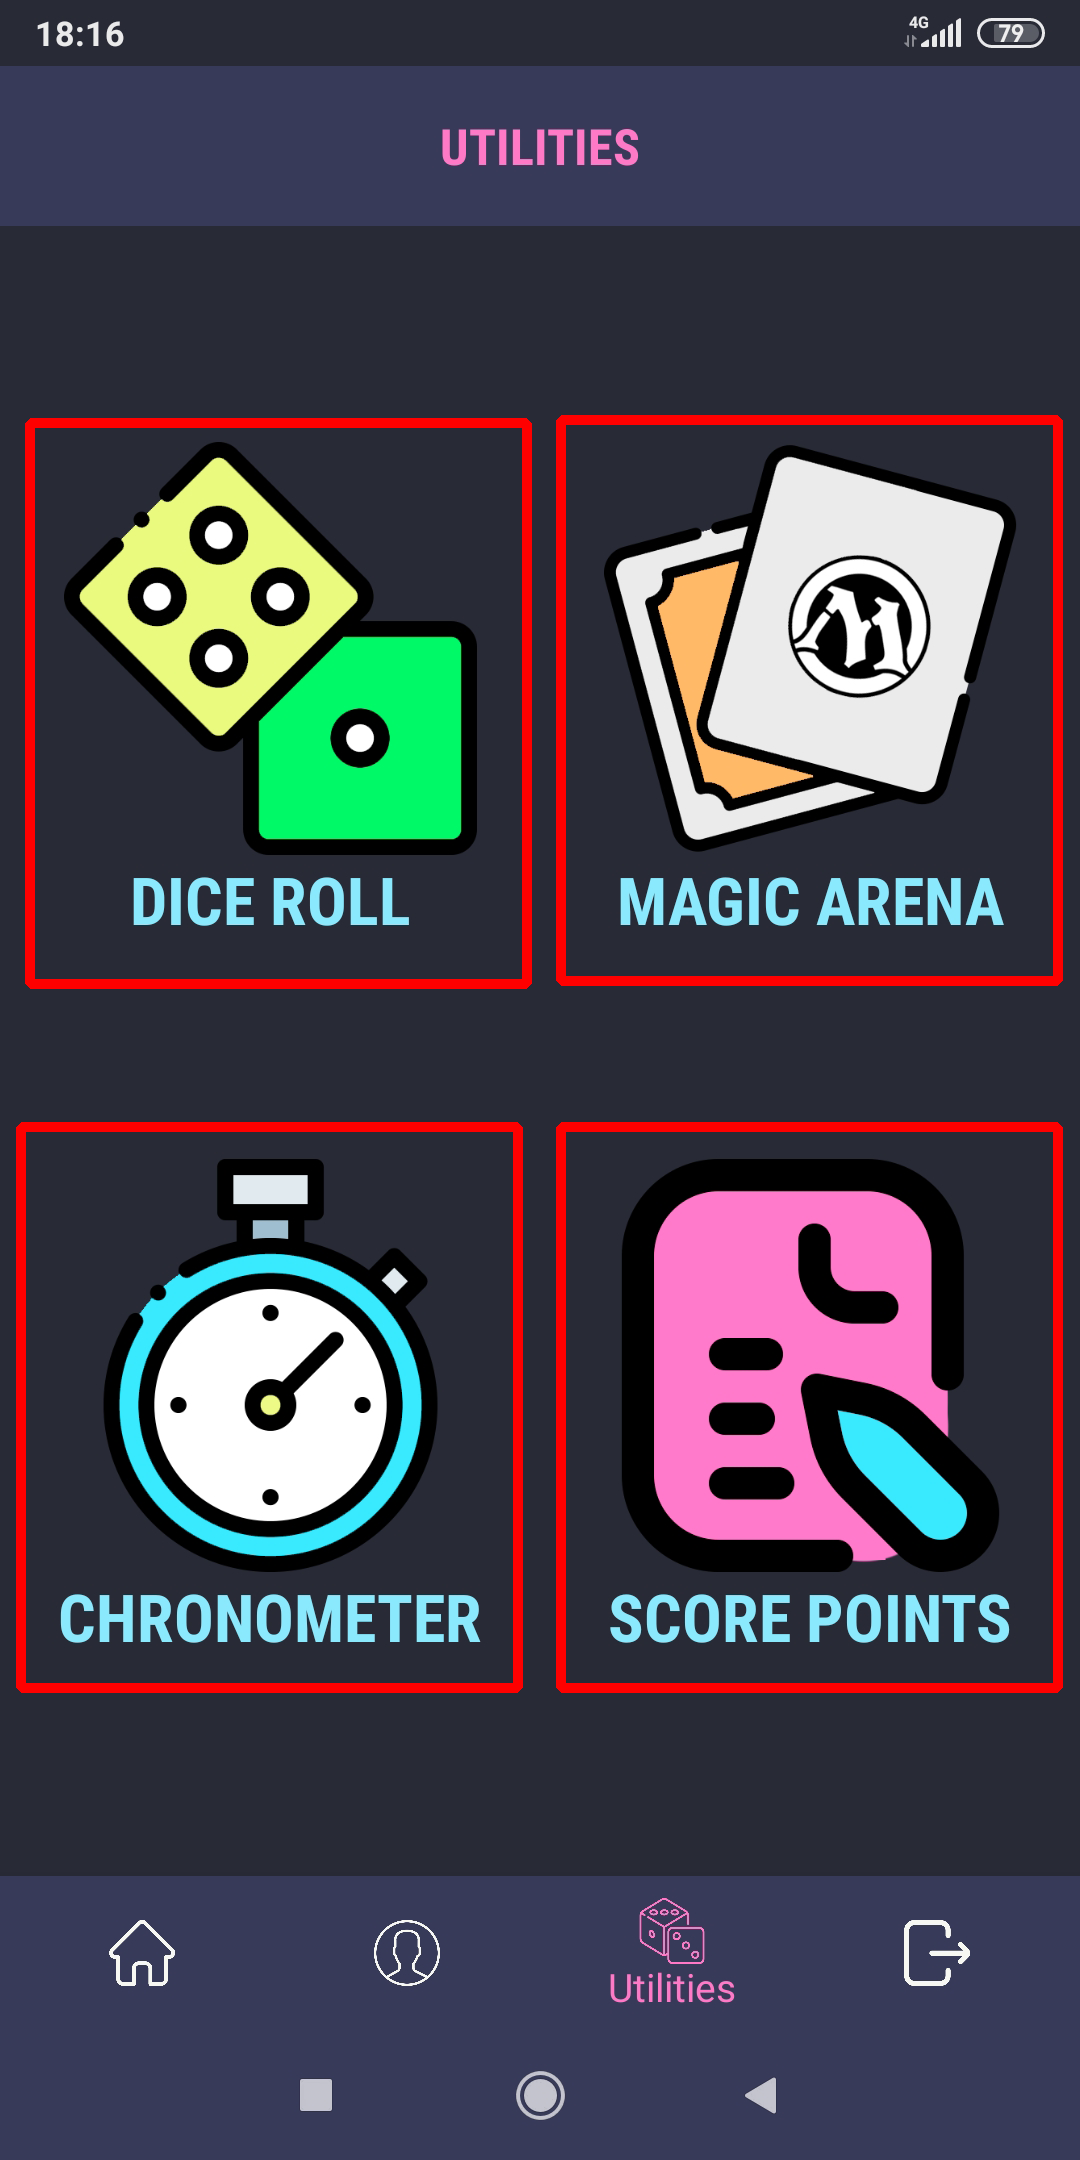
\includegraphics[width=0.3\linewidth]{fig/Uso/27.png}
    \caption{Accesos a las utilidades}
    \label{fig:uso27}
\end{figure}

Como primera utilidad tenemos \textit{Lanzamiento de dados}, que, como bien describe su nombre, sirve para lanzar dados. El número de dados y el tipo de dados se pueden ajustar mediante los botones que tendremos en la zona superior de la ventana.

\begin{figure}[H]
    \centering
    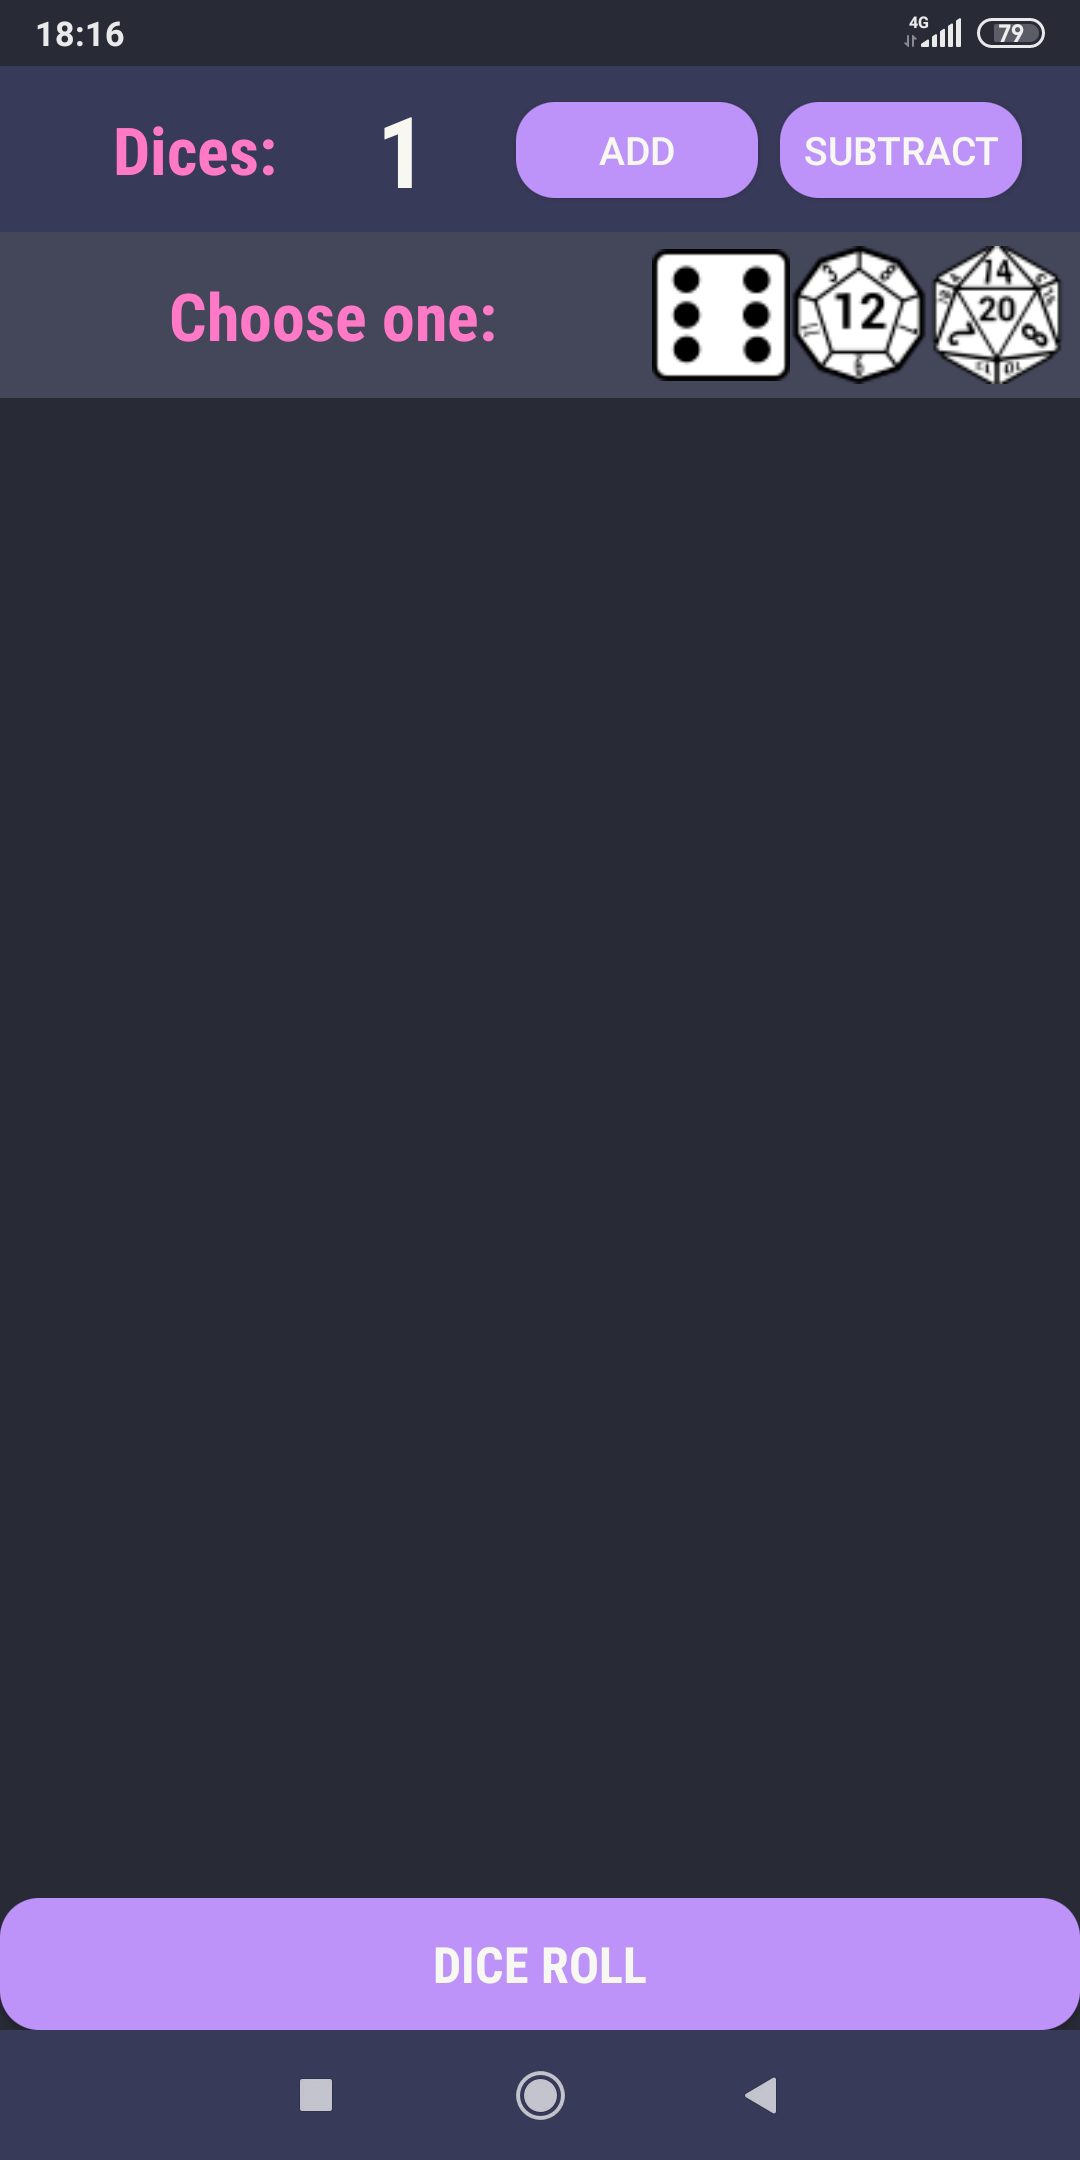
\includegraphics[width=0.3\linewidth]{fig/Uso/28.png}
    \caption{Lanzamiento de dados 1}
    \label{fig:uso28}
\end{figure}

Una vez lancemos los dados, se nos mostrará una lista con distintas caras del dado tantas veces como hayamos elegido anteriormente. Esta lista también tiene la capacidad de hacer scroll.

\begin{figure}[H]
    \centering
    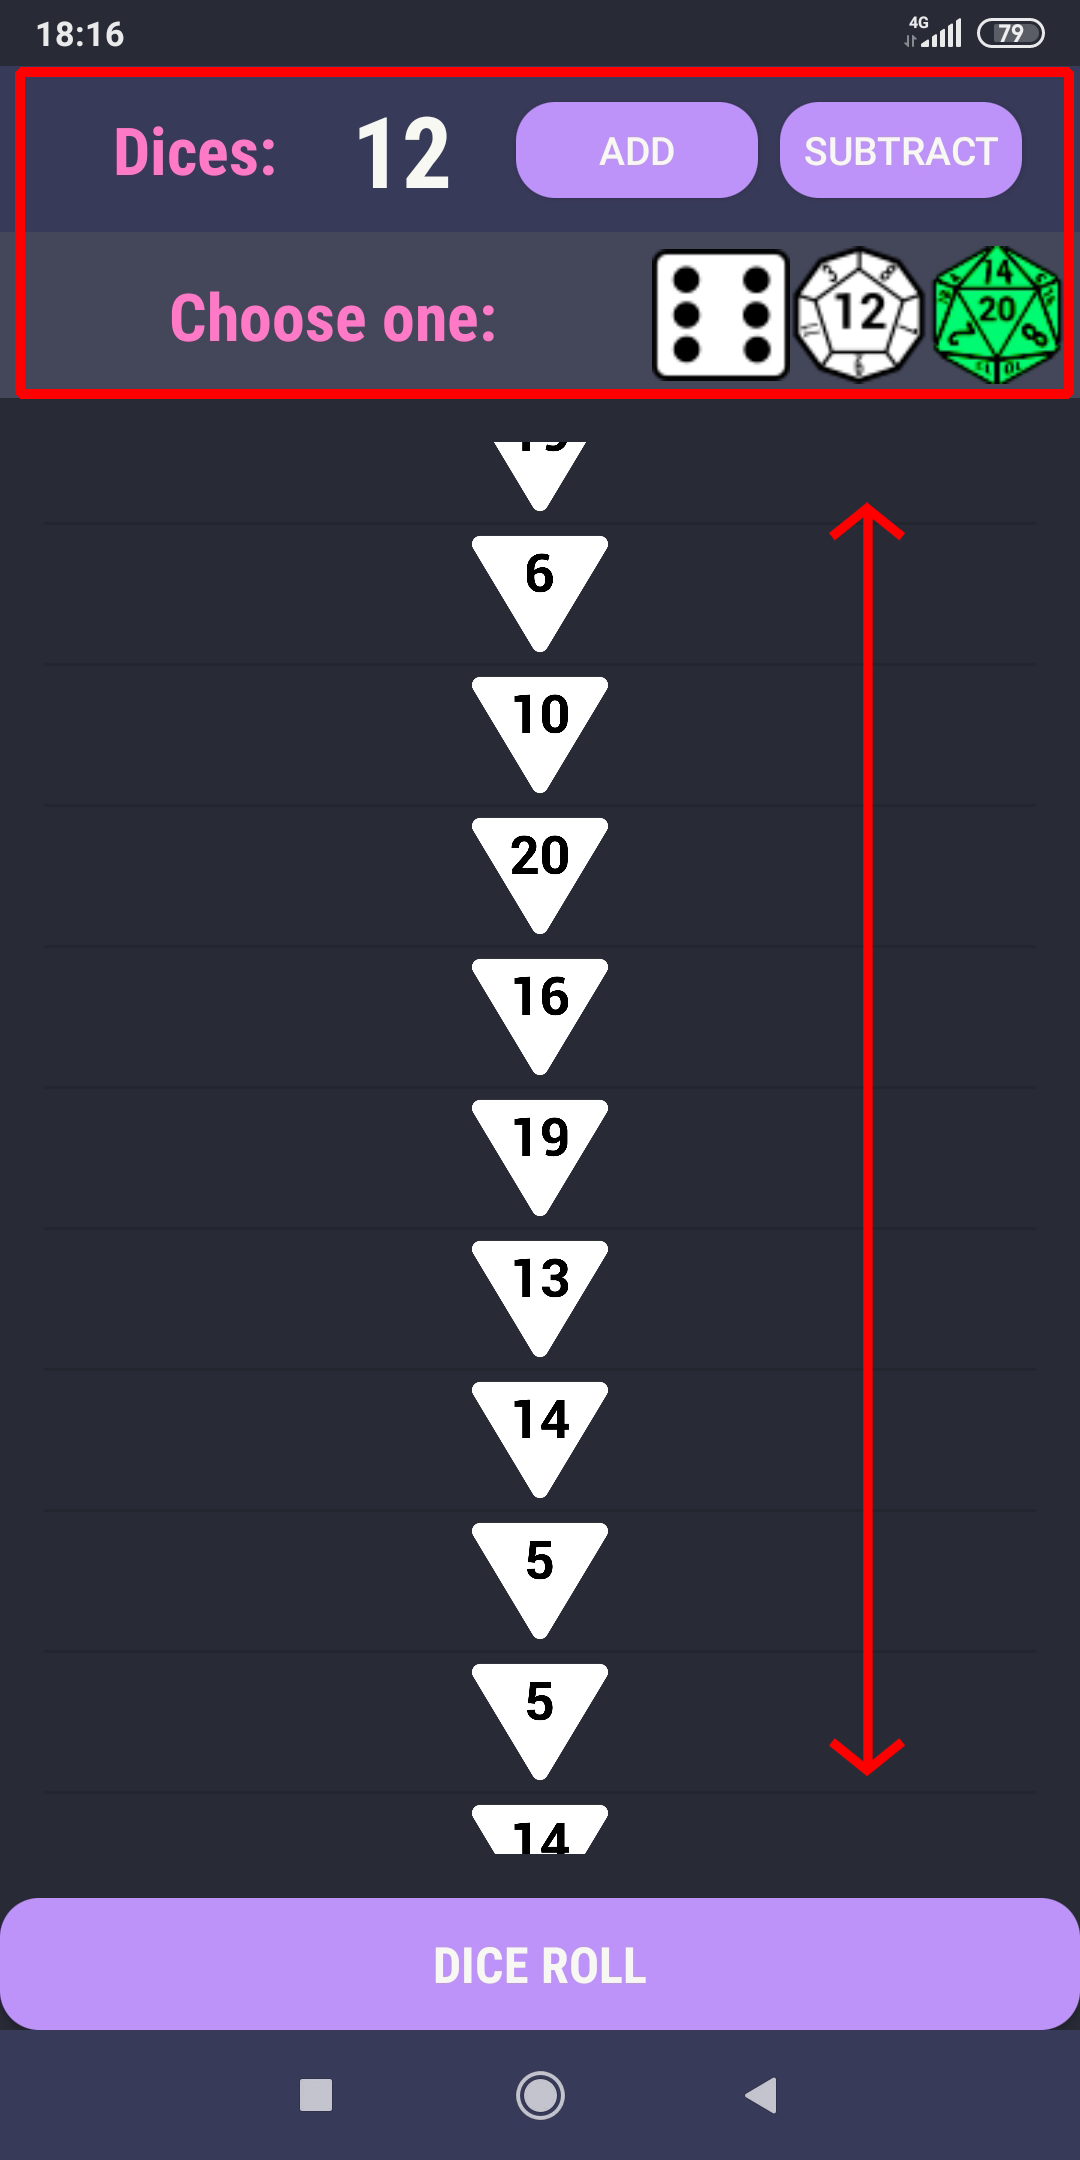
\includegraphics[width=0.3\linewidth]{fig/Uso/29.png}
    \caption{Lanzamiento de dados 2}
    \label{fig:uso29}
\end{figure}

Como segunda utilidad tenemos \textit{Magic Arena} donde se nos facilitará una serie de contadores que se pueden aumentar y disminuir de uno en uno o de cinco en cinco. Estos contadores pueden representar salud, maná, veneno, ataque, commander, etc. Todo esto depende del juego al que se esté jugando.

\begin{figure}[H]
    \centering
    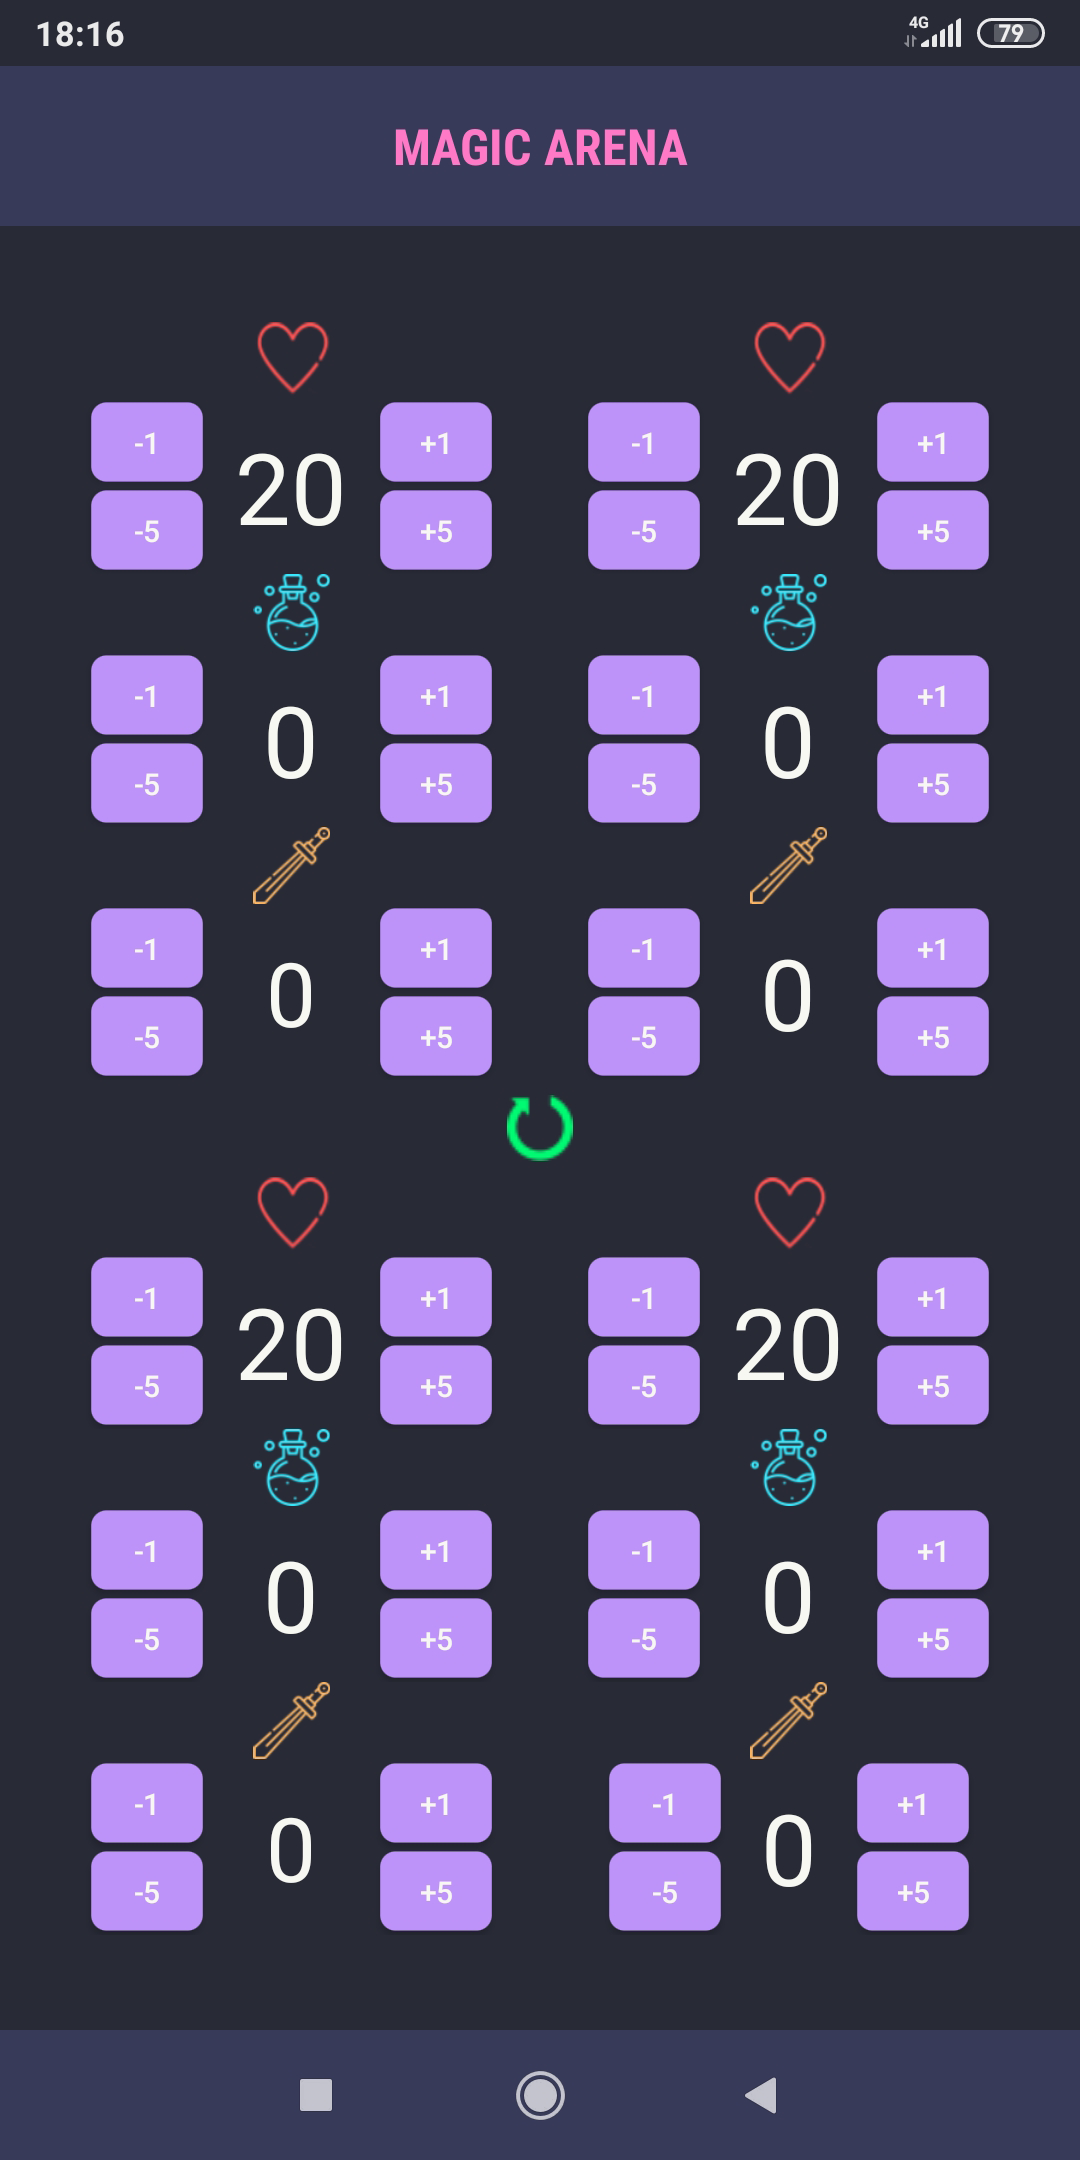
\includegraphics[width=0.3\linewidth]{fig/Uso/30.png}
    \caption{Magic Arena 1}
    \label{fig:uso30}
\end{figure}

\begin{figure}[H]
    \centering
    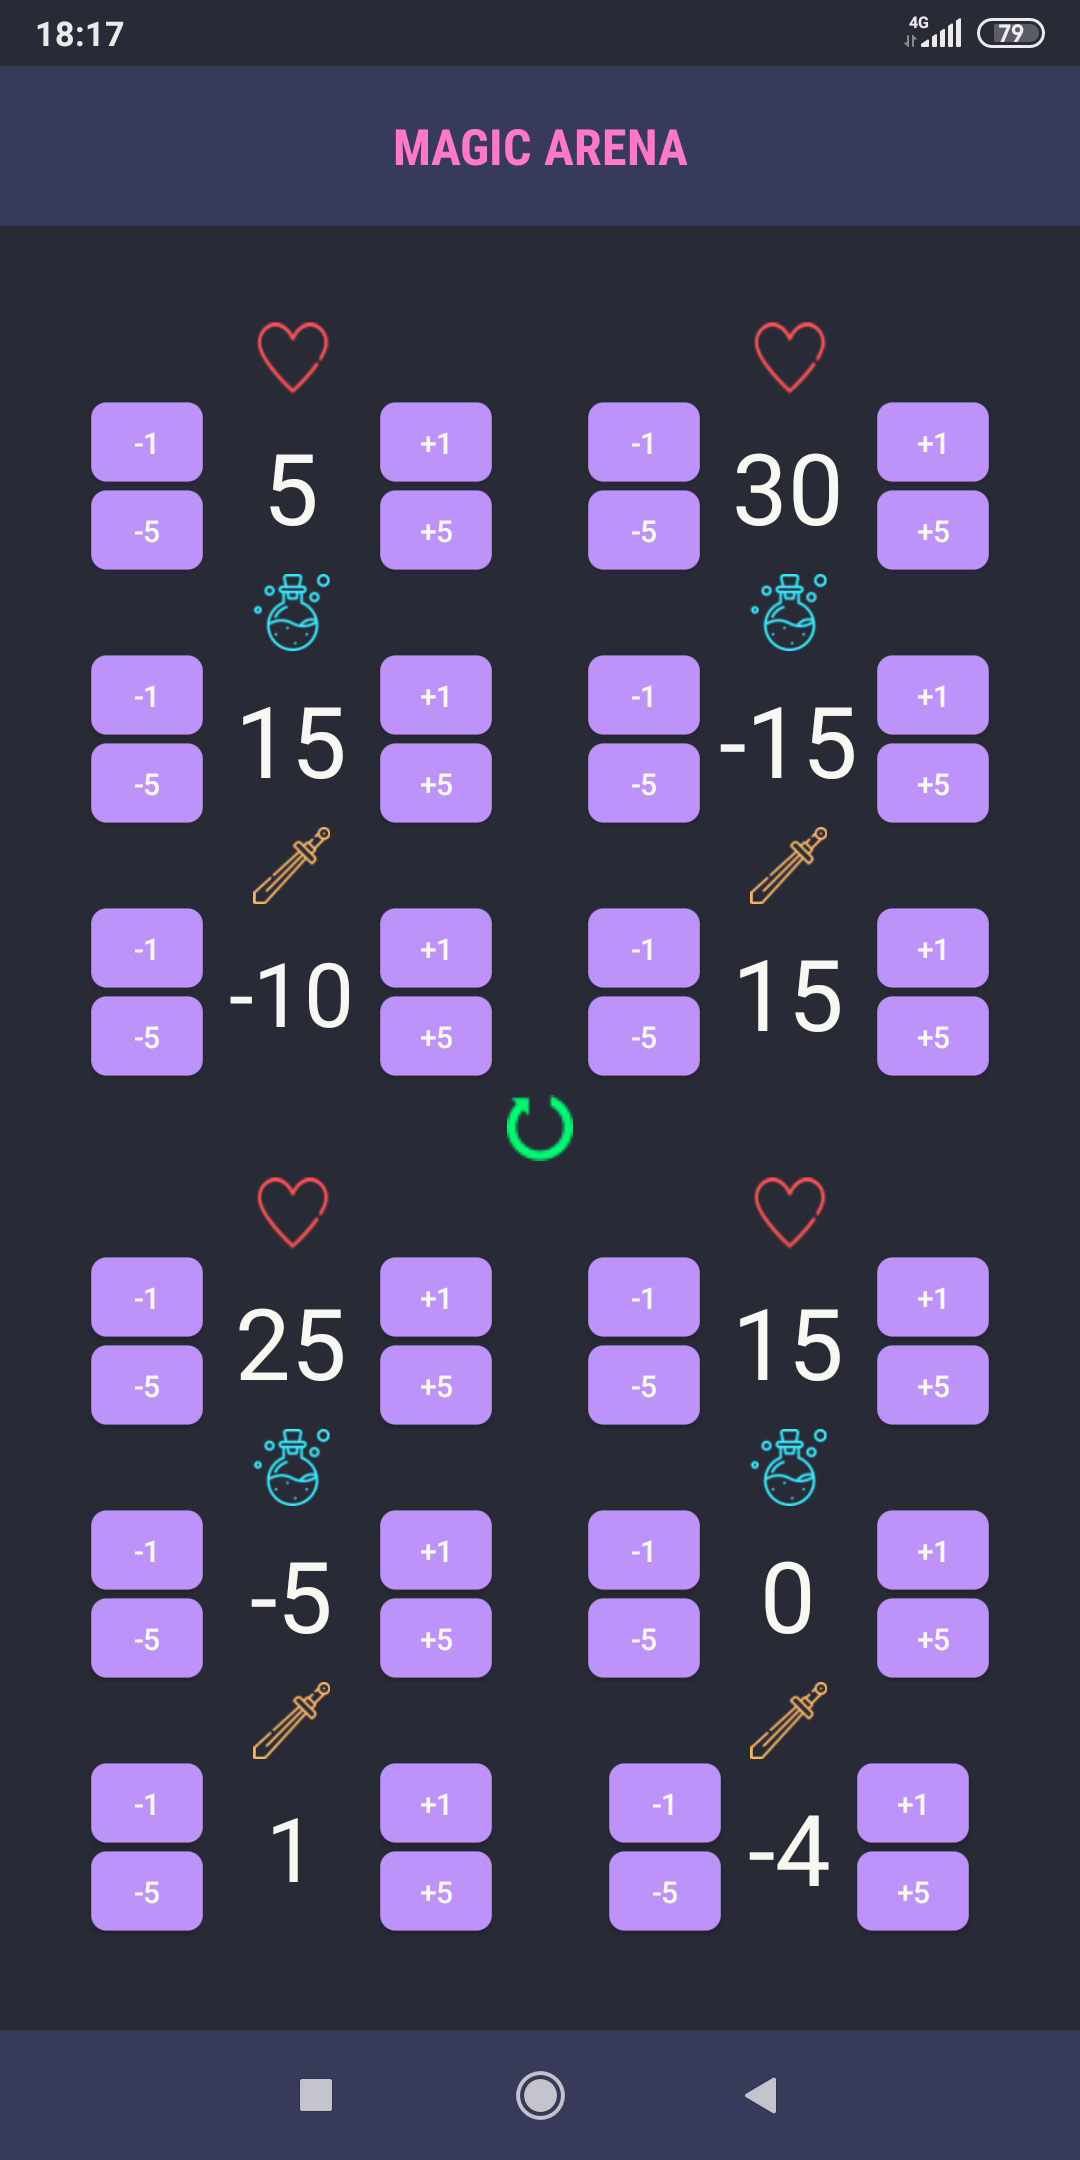
\includegraphics[width=0.3\linewidth]{fig/Uso/31.png}
    \caption{Magic Arena 2}
    \label{fig:uso31}
\end{figure}

Estos contadores se pueden restablecer sin salir de la utilidad haciendo clic sobre el botón que nos encontramos en el centro.

\begin{figure}[H]
    \centering
    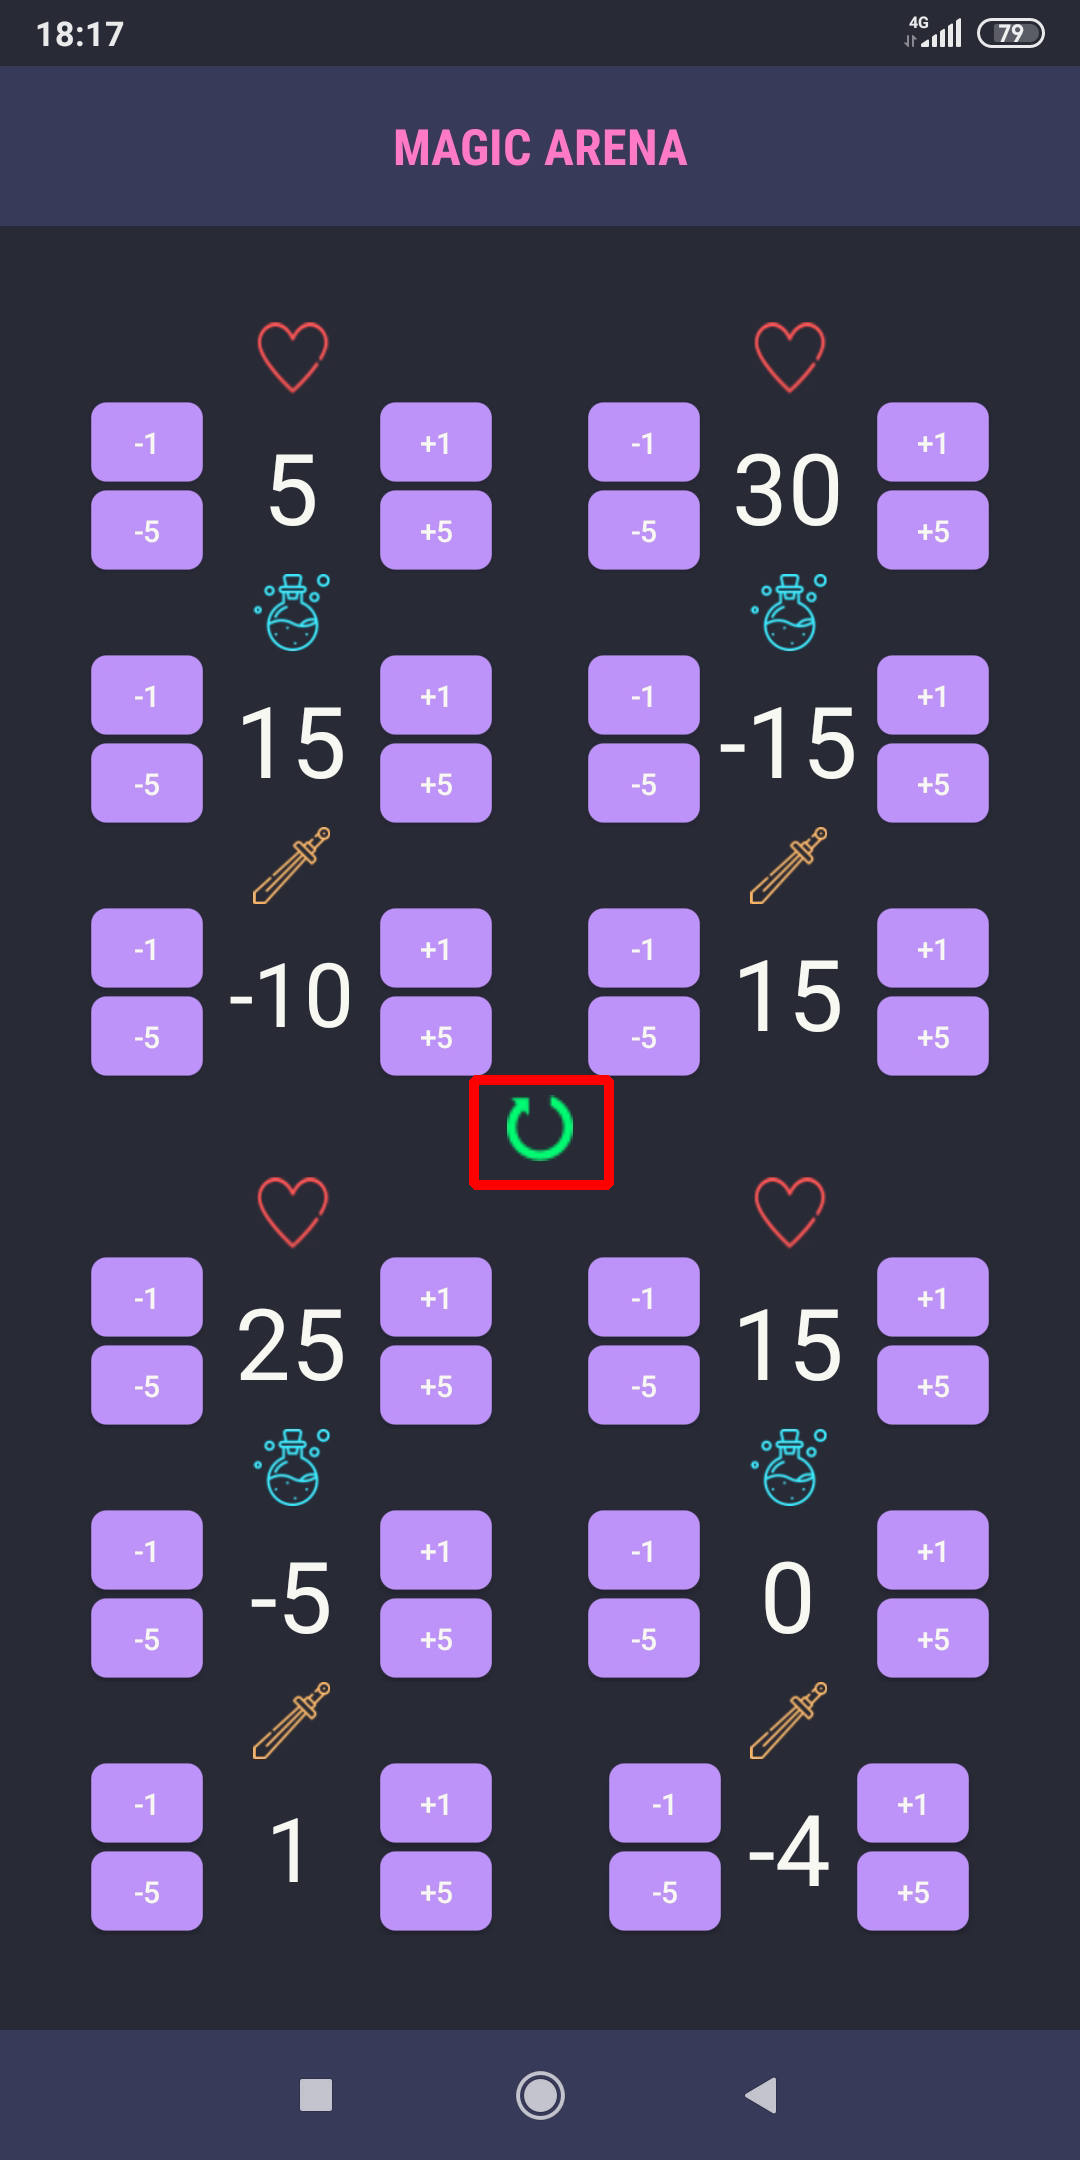
\includegraphics[width=0.3\linewidth]{fig/Uso/32.png}
    \caption{Magic Arena 3}
    \label{fig:uso32}
\end{figure}

De penúltima utilidad nos encontraremos con un simple cronómetro el cual hace la función de cronómetro: calcular el tiempo transcurrido.

En esta actividad habrá tres botones los cuales sirven para iniciar, pausar o reiniciar el tiempo.

\begin{figure}[H]
    \centering
    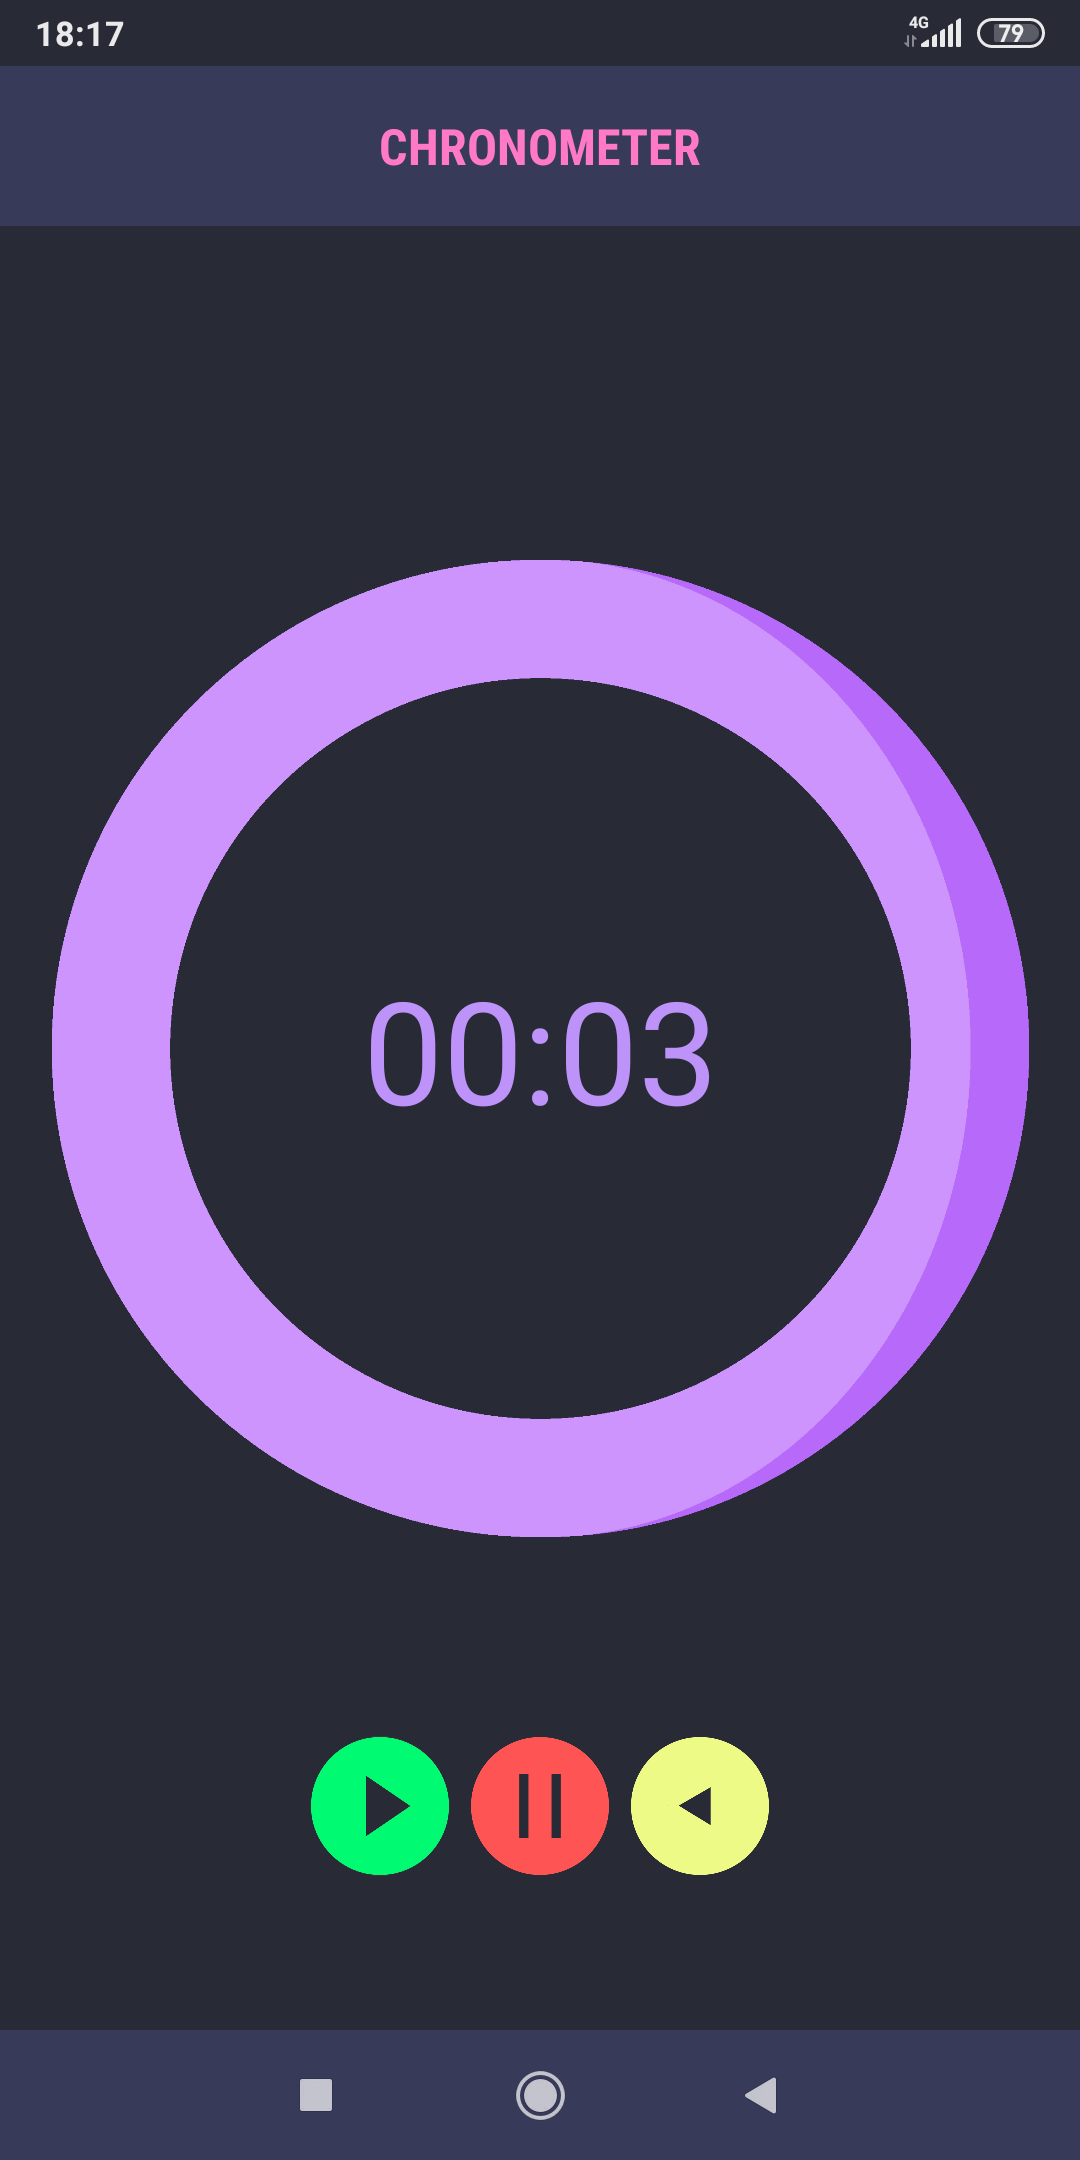
\includegraphics[width=0.3\linewidth]{fig/Uso/33.png}
    \caption{Cronómetro 1}
    \label{fig:uso33}
\end{figure}

\begin{figure}[H]
    \centering
    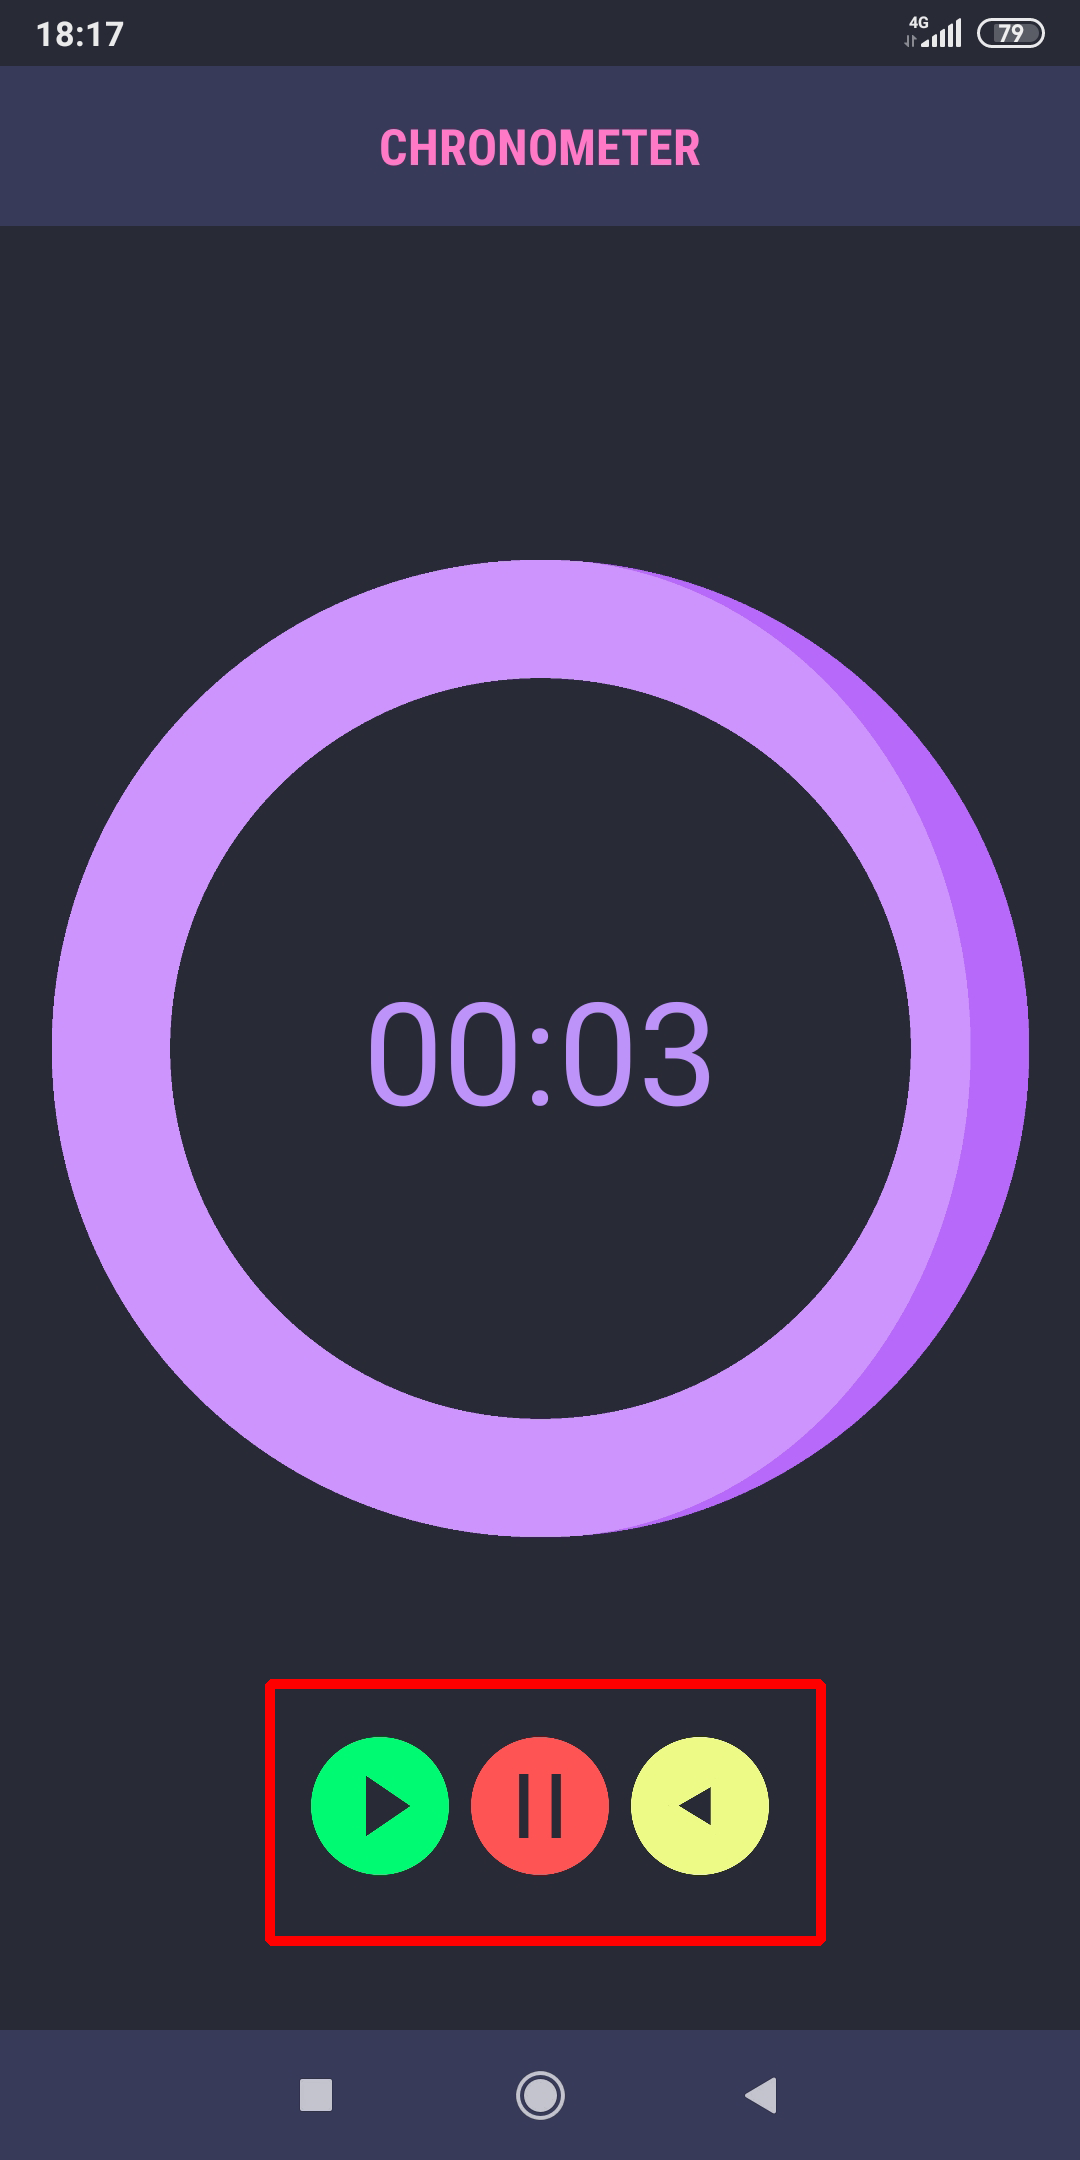
\includegraphics[width=0.3\linewidth]{fig/Uso/34.png}
    \caption{Cronómetro 2}
    \label{fig:uso34}
\end{figure}

Y de última utilidad está el \textit{registrador de puntos}. Aquí nos encontraremos con un texto que podremos modificar a un número comprendido entre 1 a 30 que especificará el número de jugadores en la partida, con lo que aparecerá, el mismo número de veces marcado, dos textos a modificar y dos botones. En estos textos tendremos que poner el nombre del jugador y su puntuación en \textit{vivo}, esto quiere decir durante el transcurso de la partida ir modificándolo. La puntuación puede ser escrita a mano (con el teclado) o haciendo uso de los botones que se proporcionan para sumar o restar de uno en uno dichos puntos.

\begin{figure}[H]
    \centering
    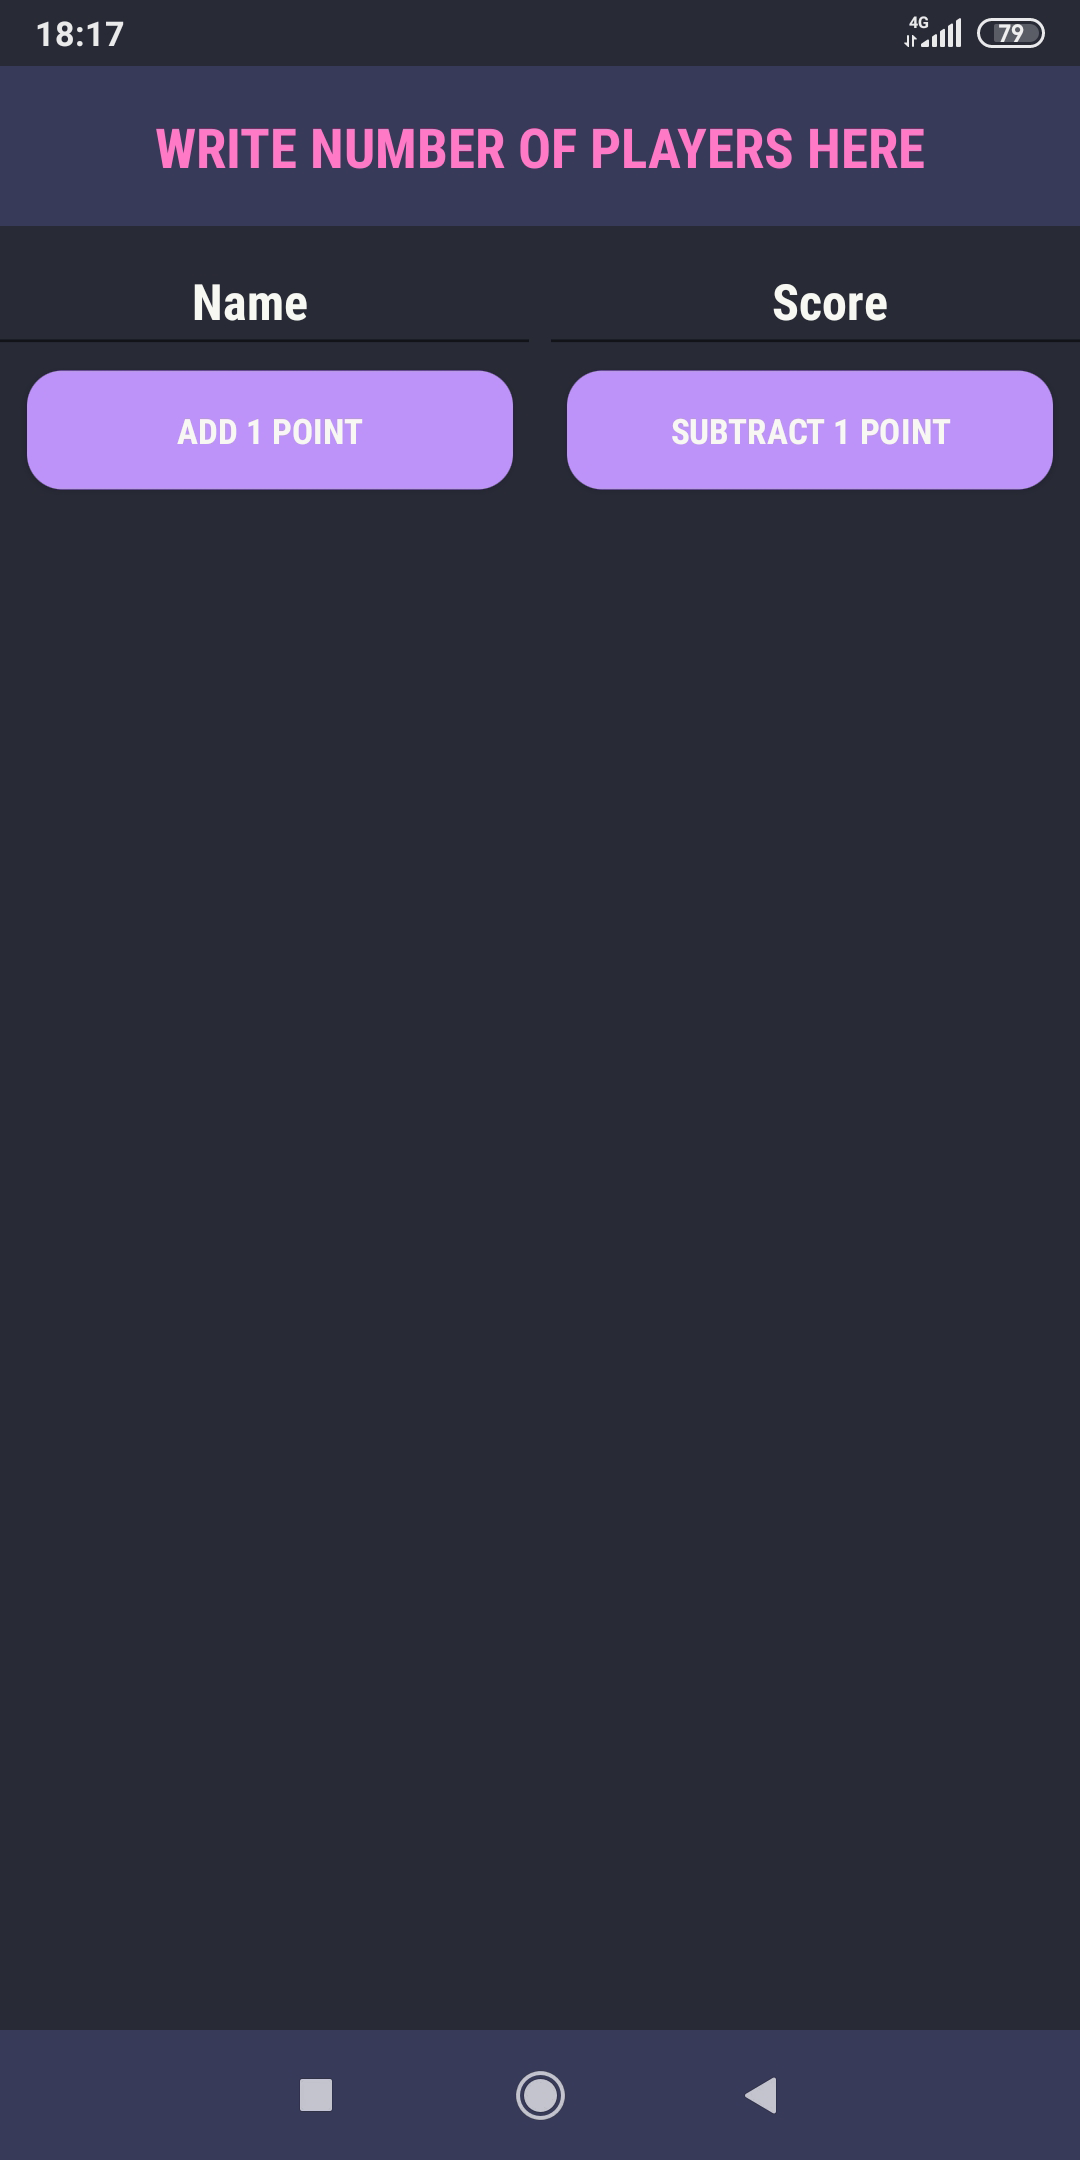
\includegraphics[width=0.3\linewidth]{fig/Uso/35.png}
    \caption{Registrador de puntos 1}
    \label{fig:uso35}
\end{figure}

\begin{figure}[H]
    \centering
    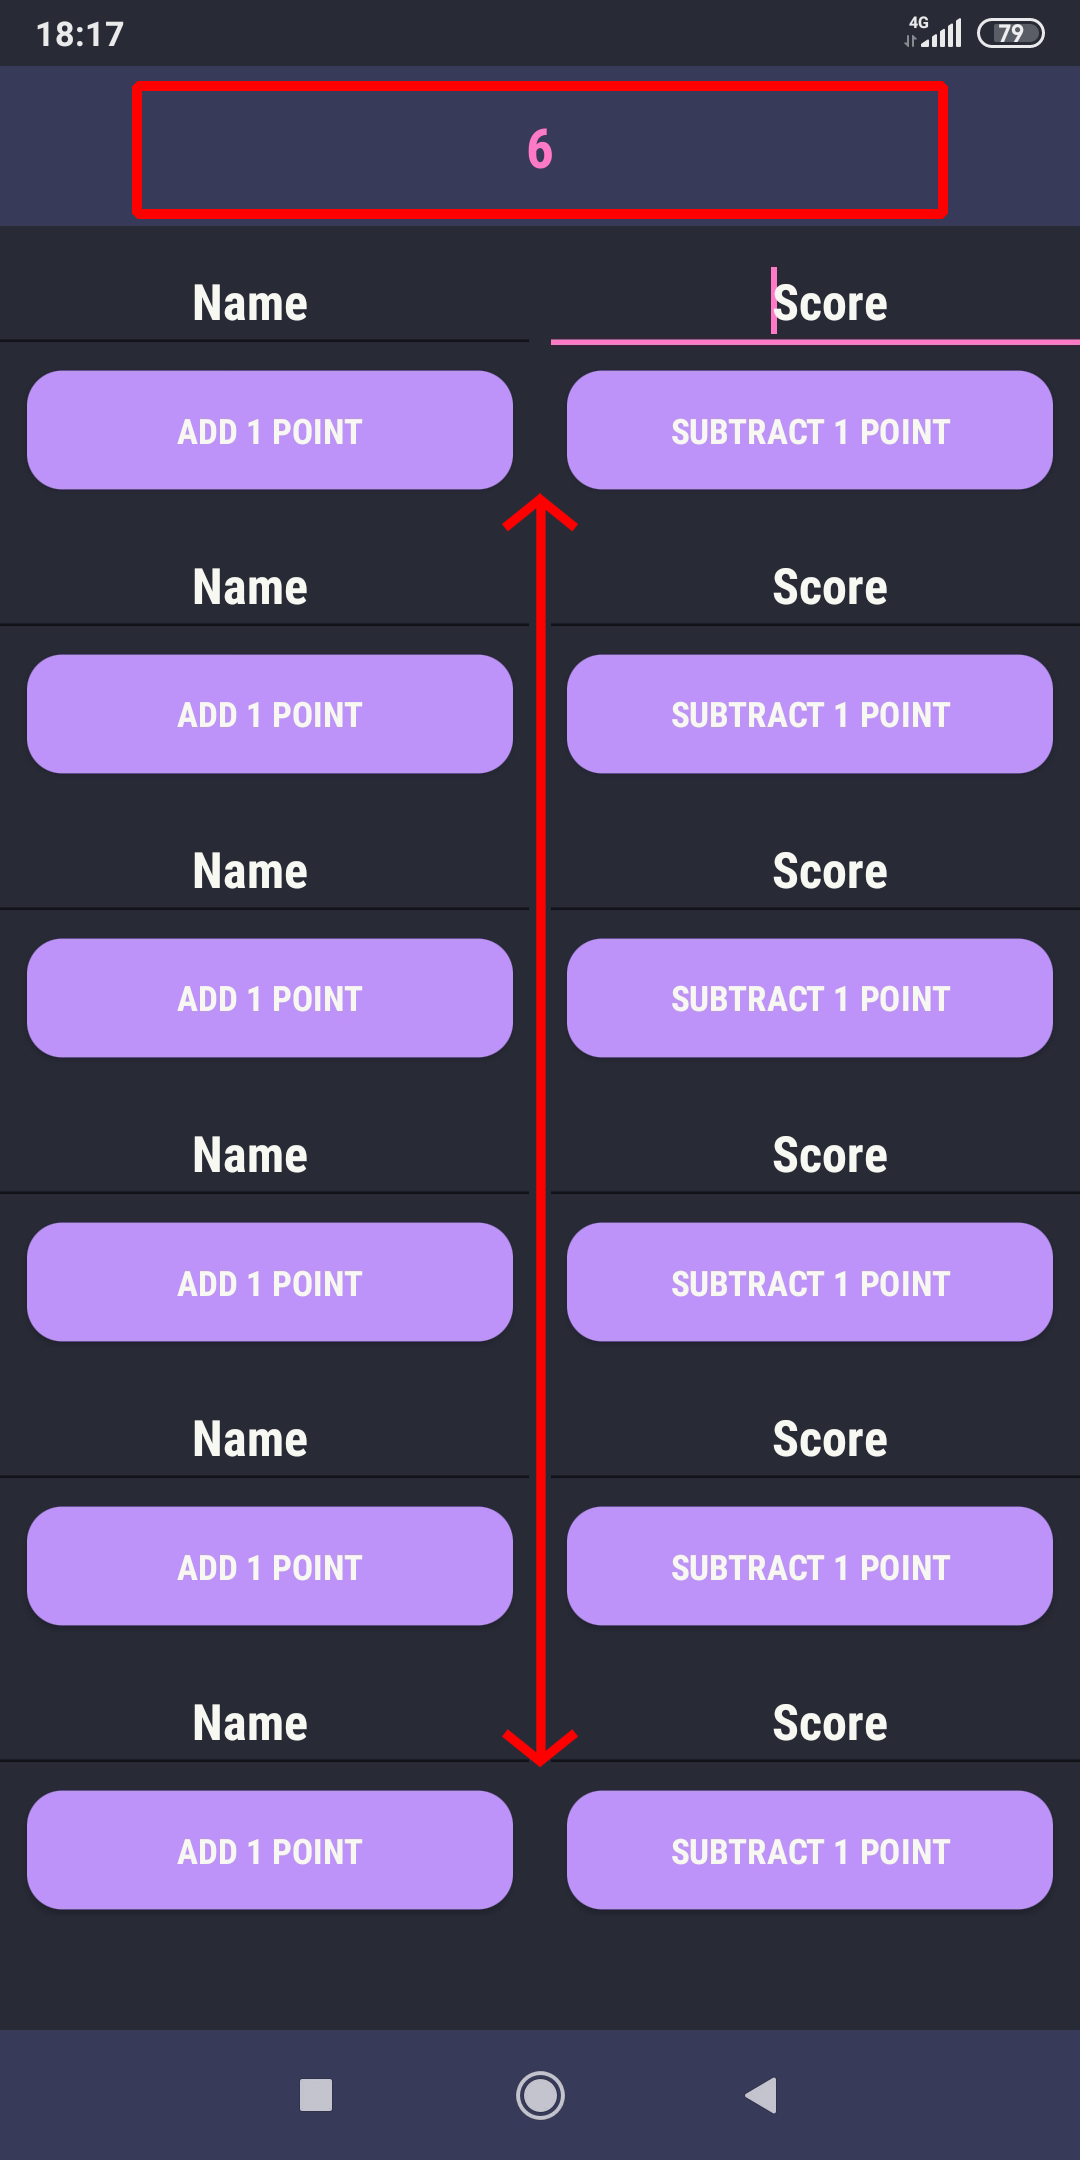
\includegraphics[width=0.3\linewidth]{fig/Uso/36.png}
    \caption{Registrador de puntos 2}
    \label{fig:uso36}
\end{figure}

\begin{figure}[H]
    \centering
    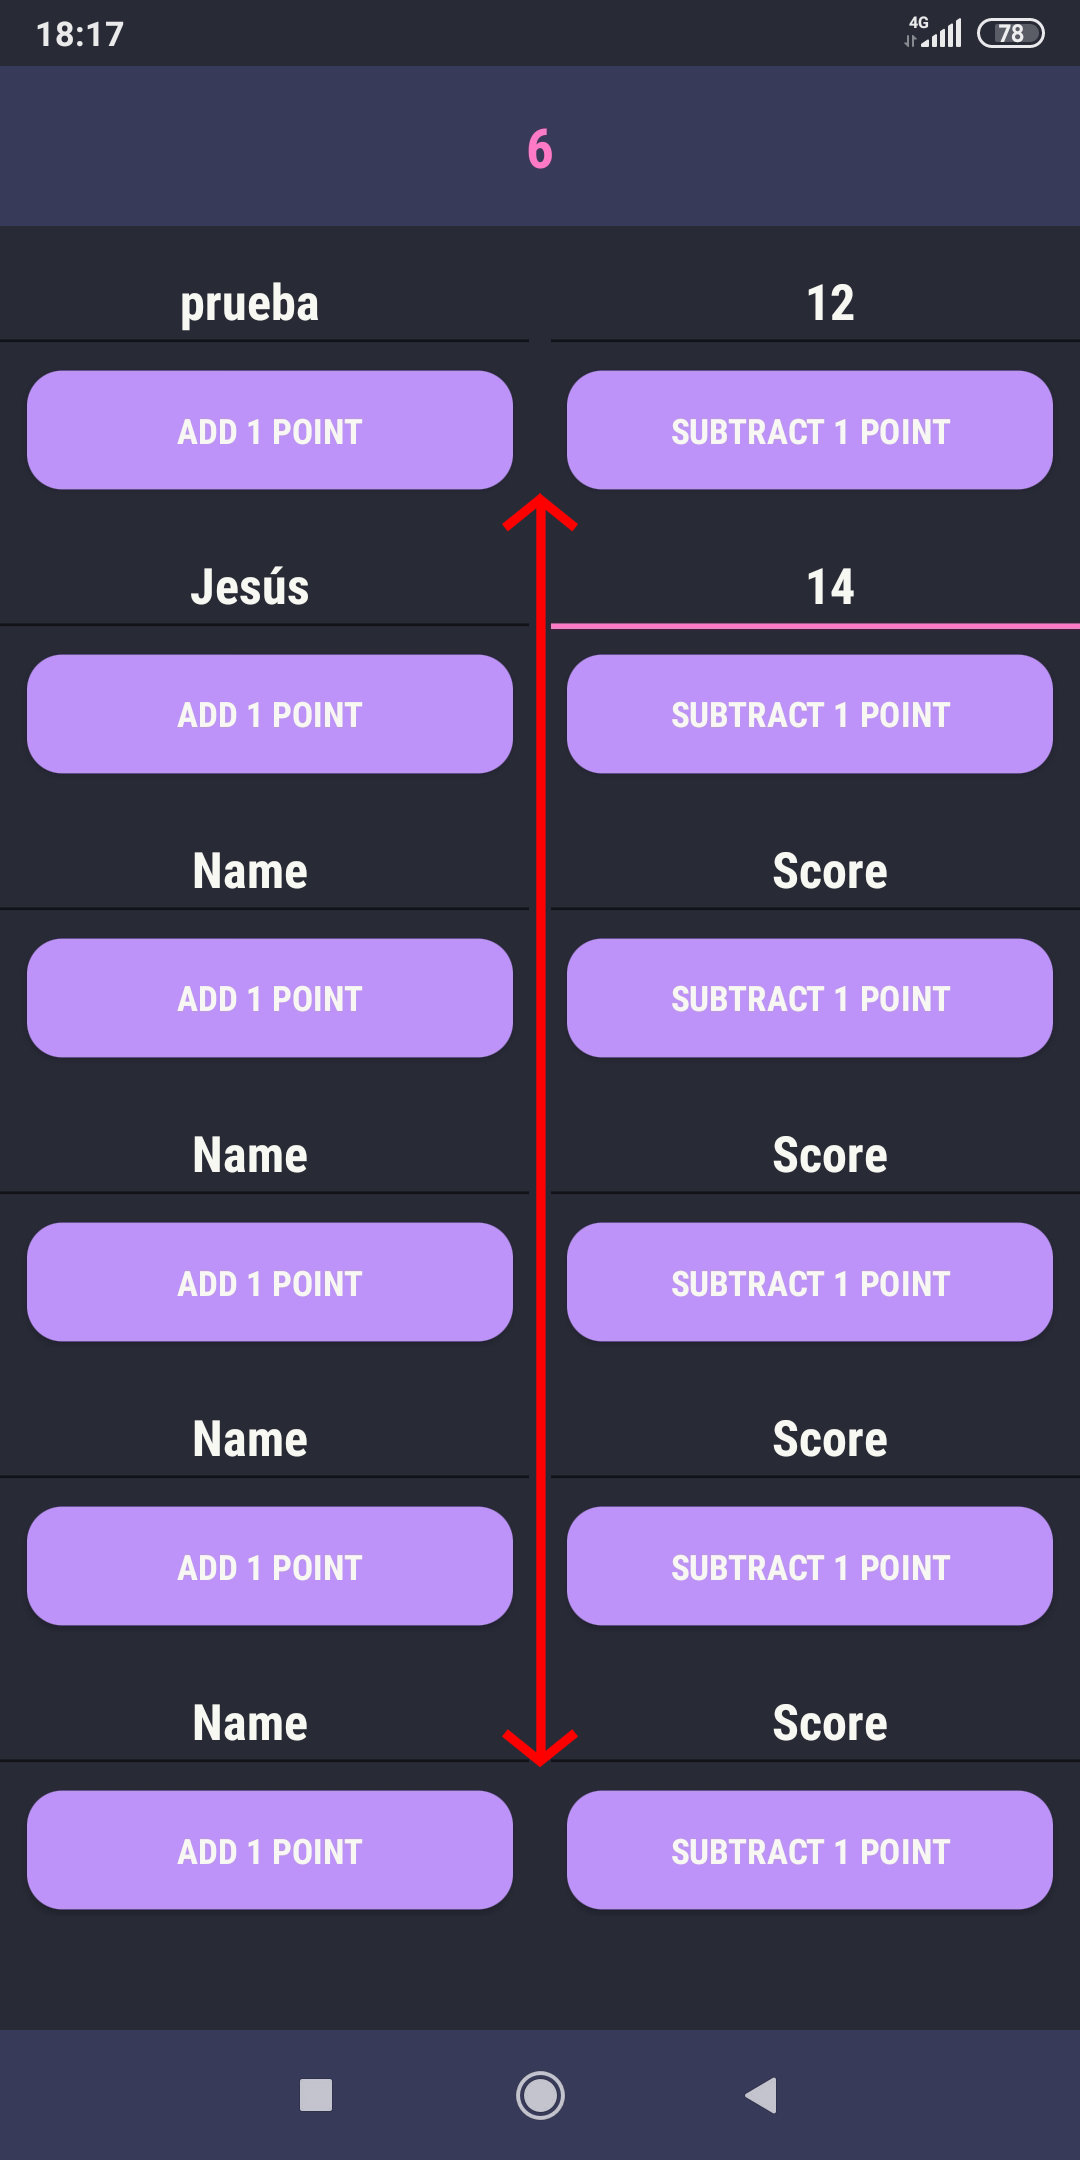
\includegraphics[width=0.3\linewidth]{fig/Uso/37.png}
    \caption{Registrador de puntos 3}
    \label{fig:uso37}
\end{figure}

% Fin del documento
\end{document}
